%===================================================================
% Chapter: GenRewrite (SIGMOD 2026 / PACMMOD)
% Sections are the final paper sources, included verbatim.
% Labels are prefixed with "gen:"; the paper's \tool macro was
% renamed to \genrewrite.
%===================================================================
\chapter{GenRewrite: Query Rewriting via Large Language Models}
\label{gen:chap}

\begingroup
\renewcommand{\thefootnote}{}%
\footnotetext{The material in this chapter is adapted from published
work: Jie Liu and Barzan Mozafari, ``GenRewrite: Query Rewriting via
Large Language Models,'' \emph{Proceedings of the ACM on Management of
Data} 4(1) (SIGMOD), Article 70, 2026~\cite{genrewrite}.}%
\endgroup

\lstset{style=genrewriteCode}

\section{Introduction}\label{gen:sec:intro}

Inefficient queries are a significant problem for nearly any organization relying on a database system. These poorly written queries—whether authored by inexperienced users or auto-generated by business intelligence (BI) tools—are a major cause of slow performance and, in cloud databases like Snowflake~\cite{dageville2016snowflake} or BigQuery~\cite{fernandes2015bigquery}, can lead to excessive costs. 
As a result, SQL-to-SQL query rewriting is a crucial step in optimizing performance and reducing expenses, 
as the likelihood of the query optimizer finding an efficient query plan is significantly diminished if it is given a poorly-written query to begin with. 
However, whether performed manually or automatically, query rewriting has remained a challenging task.

\genhead{Challenges of manual query rewriting}
The poorly-written queries that have the biggest impact on the overall cost and performance tend to be quite complex too. 
For example, it is not uncommon for queries auto generated by
Looker~\cite{lookergoogle} to span 100s of lines.
Ensuring the rewritten query preserves the semantics of the original requires a deep understanding of the database schema, constraints, and the user intent, and is therefore a time-consuming and error-prone task, even for seasoned database experts.
The fact that there are often thousands, if not millions, of such slow queries makes the manual approach a monumental undertaking.

\genhead{Limitations of traditional automated query rewriting} 
Despite extensive research, automated query rewriting techniques have long faced fundamental limitations that hinder their practical effectiveness. The most common approach relies on \emph{rewrite rules}—--pattern-matching transformations that replace query fragments with optimized equivalents while preserving semantics. 
Regardless of whether the rules are developed and provided by experts~\cite{bruno2022computation,pirahesh1992extensible,ahmed2006cost} or 
are inferred automatically~\cite{wetune,ding2023proving},
a rule-based query rewriter is as effective as the set of rules provided to it. 
By definition, rule-based query rewriters\footnote{Rule-based query \emph{rewriting} should not be confused with rule-based query \emph{optimization}; the latter is simpler, and thus much more common in practice~\cite{graefe1987rule}.}
% are limited to situations where the input query matches one of their existing rules,  
% and thus
are fundamentally incapable of optimizing new query patterns that do not match their existing rules~\cite{dong2023slabcity}.
Although synthesis-based query-rewriting does not require prior rules~\cite{dong2023slabcity}, in practice it only handles simple queries---for instance, SlabCity~\cite{dong2023slabcity} optimizes just 2 out of 22 TPC-H~\cite{tpch} queries and 3 out of 99 TPC-DS~\cite{tpcds} queries.



\begin{comment}

\begin{table*}[htbp]
\centering
\label{gen:tab:plan_templates}
\begin{tabular}{|c|c|c|c|}
\hline
\textbf{No.} & \textbf{Source Query Pattern} & \textbf{Destination Query Pattern} & \textbf{Constraints} \\
\hline
1 & $\operatorname{Sel}_{\mathrm{p}, \mathrm{r} . \mathrm{a}_0}(\operatorname{Proj}_{\mathrm{r} . \mathrm{a}_1}(\mathrm{r}))$ & $\operatorname{Proj}_{\mathrm{r} . \mathrm{a}_1}(\operatorname{Sel}_{\mathrm{p}, \mathrm{r} . \mathrm{a}_0}(\mathrm{r}))$ & $\operatorname{SubAttrs}(a_0, a_1)$ \\
\hline
2 & $\operatorname{Proj}_{\mathrm{r} . \mathrm{a}_0}(\operatorname{Sel}_{\text {p,r. } \mathrm{a}_1}(\text { Proj }_{\mathrm{r} . \mathrm{a}_2}(\mathrm{r})))$ & $\operatorname{Proj}_{\mathrm{r} . \mathrm{a}_0}(\operatorname{Sel}_{\mathrm{p}, \mathrm{r} . \mathrm{a}_1}(\mathrm{r}))$ & $\operatorname{SubAttrs}(a_0, a_2), \operatorname{SubAttrs}(a_1, a_2)$ \\
\hline
3 & $\text { LJoin }_{\mathrm{r}_0, \mathrm{a}_0, \mathrm{r}_1 \cdot \mathrm{a}_1}(\mathrm{r}_0, \mathrm{r}_1)$ & $\text { IJoin }_{\mathrm{r}_0 \cdot \mathrm{a}_0, \mathrm{r}_1 \cdot \mathrm{a}_1}(\mathrm{r}_0, \mathrm{r}_1)$ & $\operatorname{RefAttrs}(\mathrm{r}_0, \mathrm{a}_0, \mathrm{r}_1, \mathrm{a}_1), \operatorname{NotNull}(\mathrm{r}_0, \mathrm{a}_0)$ \\
\hline
\end{tabular}
\caption{Examples of rewrite rules in WeTune~\cite{??}}
\end{table*}



\begin{enumerate}
    \item \textbf{Semantic side}: Ensuring that the rewrite preserves the semantics of the original query is crucial, which requires a deep understanding of the database schema, constraints, and the query intent.
    \item \textbf{Syntax side}: SQL queries and database schemas can be both highly complex. Manipulating their elements without introducing errors requires sophisticated analysis.
\end{enumerate}
\end{comment}

% \genbarzan{use either Text-to-SQL or Natural Language to SQL (NL2SQL) consistently everywhere in the paper}

% a few other 
% \genbarzan{would be better to name those areas here and cite them, e.g., blah~\cite{`}, blah~\cite{} and blah~\cite{}}
% areas~\cite{citeALlOtherPapersThatHaveAppliedLLMsToADBProblemExceptTheTextToSQLAndTheVisionPaperYouSentLastNight}, 

\genhead{Large language models (LLMs)} The shining success of large language models (LLMs) in performing complex and open-ended tasks has created new hopes for solving some of the hardest database problems as well. 
While researchers have used LLMs for Text-to-SQL~\cite{fu2023catsql,gao2023text,sun2306sql,katsogiannis2023survey,pourreza2024din} and a few other areas, e.g., data cleaning and integration~\cite{narayan2022can,suhara2022annotating}, table processing~\cite{li2023table,lu2024large} and database diagnosis~\cite{zhou2023d}, their potential for query rewriting has remained largely unexplored. In instances where human experts or existing rules cannot rewrite a query, say for complex queries or new query patterns, 
 could LLMs be leveraged to uncover rewrite opportunities due to their broad general knowledge and advanced reasoning capabilities? If so, this could drastically lower the burden on human experts and allow for a much larger set of queries to benefit from rewriting.
To the best of our knowledge, this paper is the first\footnote{See \S\ref{gen:sec:related} for related work published after the initial publication of our work on ArXiv.} to focus on 
 answering this question: how to best leverage LLMs for query rewriting beyond rules and how to address the challenges involved.

\genhead{Challenges} Using LLMs for query rewriting has challenges:\footnote{A common misunderstanding is that the time and monetary overhead of invoking an LLM may outweigh the speedup benefits of the rewrite. However, this one-time overhead is less relevant for repetitive workloads, which are the focus of \genrewrite (see \textbf{Target workloads}).} 
\begin{enumerate}[label=C\arabic*, leftmargin=0.5cm]

\item The na\"ive  approach of simply prompting the LLM to "rewrite the given query into a faster but equivalent form"  can rarely handle complex queries: 
most outputs either fail to parse (syntactic errors) or produce incorrect results (semantic errors) due to SQL’s complexity and LLM hallucinations (\S~\ref{gen:sec:expr:llmbaseline}).
%~\cite{zhang2023siren,tonmoy2024comprehensive}.

\item LLMs lack a database cost model and cannot run experiments, so their rewrites are not necessarily faster than the original queries.

\item While LLM costs for rewriting a recurrent workload can be amortized, excessive invocations can still become expensive.
     
\item Hints can help the LLM, but excessive or irrelevant ones can lead to mistakes.

\item Due to their black-box nature, LLM rewrites are harder for humans to understand and verify than traditional  rules.

\end{enumerate}

%ta inja
\genhead{Our approach}
To address the above challenges, we present \textbf{\genrewrite}, the first holistic system that leverages LLMs for query rewriting. 
We introduce the notion of a Natural Language Rewrite Rule (NLR2), which is a textual explanation summarizing the rewrite. 
We use the LLM itself to produce the NLR2s, which are then used for three purposes. The NLR2s 1)  serve as hints assisting the LLM to provide better rewrites 
(C2), requiring fewer follow-up LLM invocations (C4), 2) make the rewrites easier to understand and verify by offering a human-readable explanation (C5), and, 
most importantly, 3) allow \genrewrite to transfer the knowledge gained from rewriting one query to another and thus become smarter and more effective over time (C1, C2, C3). Since NLR2s are void of confidential information (such as column or schema names), one can even bootstrap \genrewrite's NLR2 repository for a new workload using the repository of a previously trained \genrewrite on another workload.

To avoid redundant rules, which can in turn confuse the LLM, we maintain
    a utility score for each NLR2 to supply only those rules to the LLM  as hints that are most relevant to the query at hand.
Finally, to minimize the LLM cost and minimize the human effort needed for manual verification, 
\genrewrite does not discard incorrect rewrites. Instead, it uses a novel counterexample-guided technique to iteratively
    correct the syntactic and semantic errors in the rewritten query (C1, C3).

\begin{figure}[ht]
\inv\sinv
  \centering
  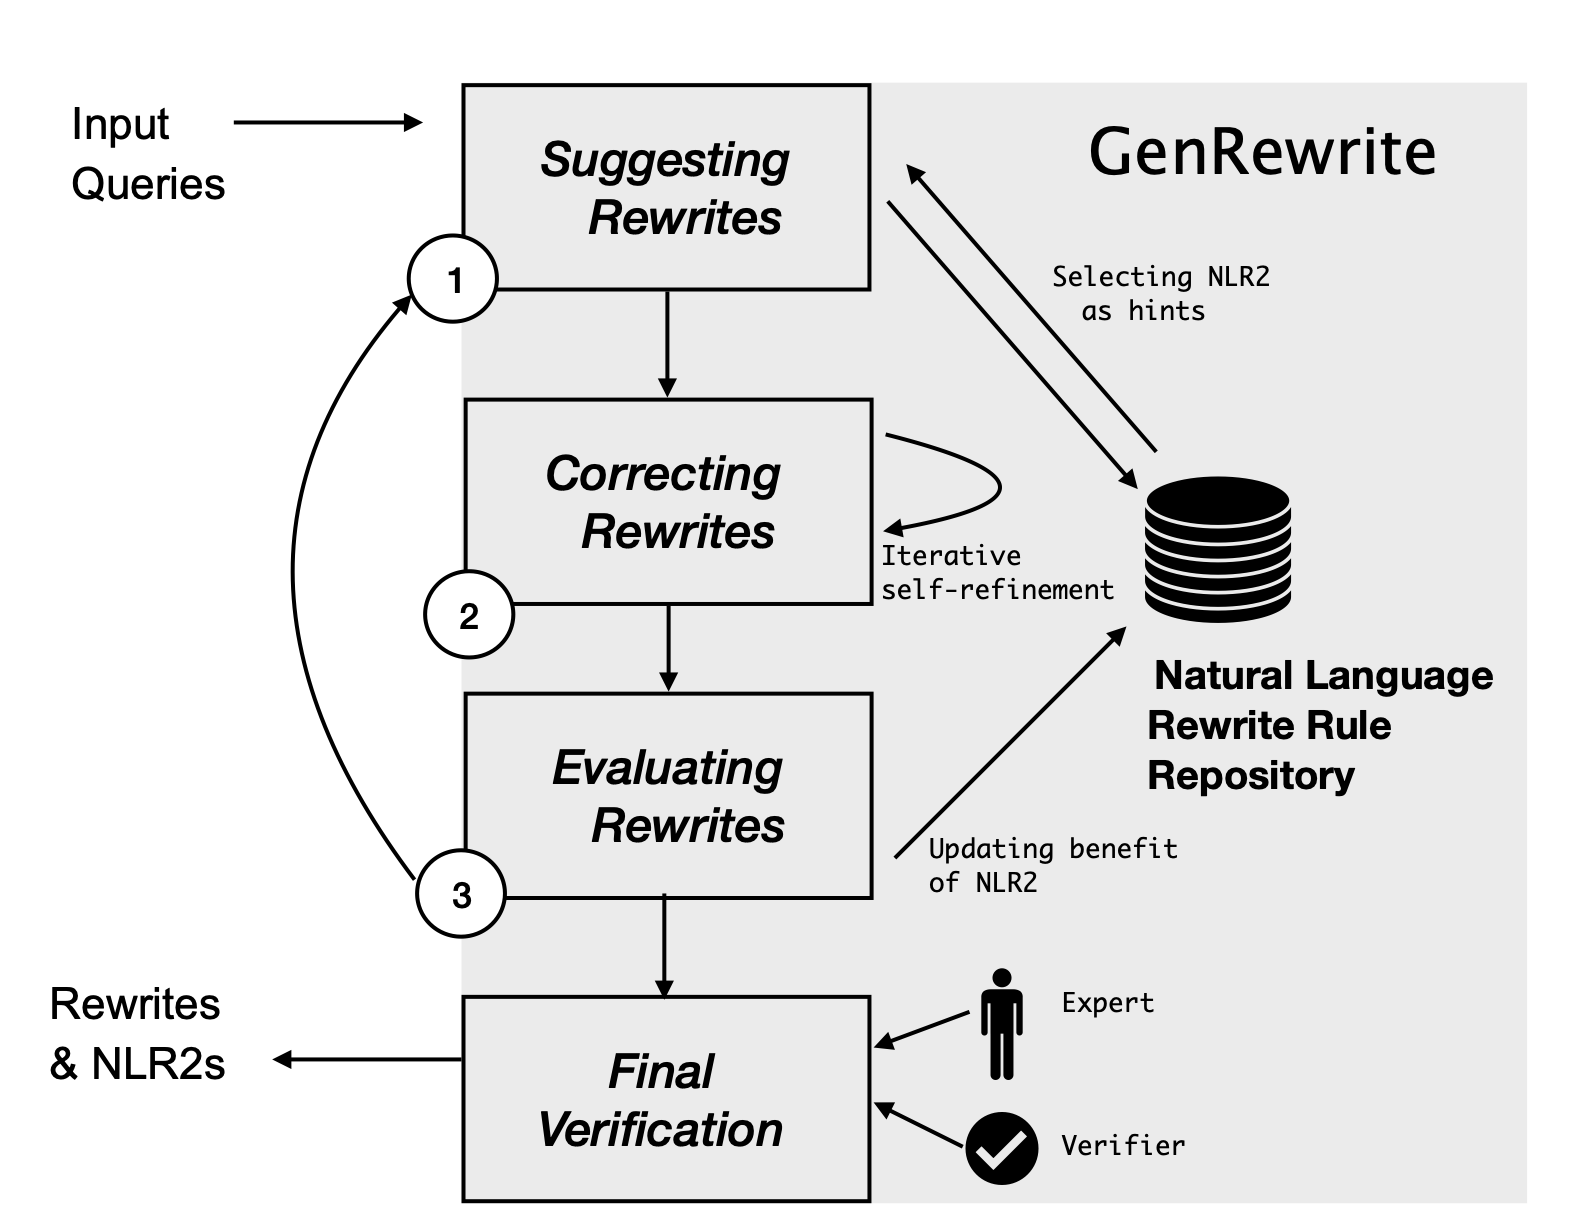
\includegraphics[width=0.8\linewidth]{chapters/genrewrite/figures/workflow.1.png}
\inv\inv
  \caption{High-level Workflow of \genrewrite }
  \label{gen:fig:arch}
\inv
\end{figure}

% \genbarzan{don't forget to fix the plot. sent you a bunch of feedback on this yesterday} \genjie{btw it is really easy to get lost in voice msgs on whatsapp, could you please remind me of the problems of this figure if you still remember}


\genhead{High-level workflow} 
\genrewrite takes as input a workload,\footnote{A streaming setting is a special case, whereby queries are presented and rewritten one at a time.}
expressed as a set of input queries $\mathcal{Q}$, and returns
\{($q$,$q'$,$e$) \textbar  $q$ $\in$ $\mathcal{Q}_{opt}$ \}, where
  $\mathcal{Q}_{opt}\subseteq \mathcal{Q}$ is the optimizable subset of the input queries, 
  $q'$ is the rewritten query that is equivalent to $q$ but likely to run faster, and $e$ is 
 a human-readable explanation of the rewrite.
Figure~\ref{gen:fig:arch} shows the overall workflow, which is an iterative process.
In each iteration, every query in the workload goes through three phases to find a better rewrite than the one found in previous iterations:
{\small \Circled{1}}  rewrite suggestion, {\small \Circled{2}}  rewrite correction, and {\small \Circled{3}}  rewrite evaluation. 
Additionally, \genrewrite \revthree{maintains} a Natural Language Rewrite Rule (NLR2) repository for knowledge transfer across queries in the workload.
{\small \Circled{1}} selects appropriate NLR2s from the repository to serve as hints for suggesting new rewrites. Any newly discovered NLR2 is also added to the repository. 
{\small \Circled{2}} iteratively refines rewrites based on the counterexamples provided by the LLM  to eliminate semantic and syntactic errors.
  {\small \Circled{3}} evaluates the rewrites for equivalence and performance, and updates the benefit score of the used NLR2s accordingly.
This process continues until no additional improvement is found and the set of rewrites stabilizes. 
The rewrites then go through a final verification step {\small \Circled{4}}, 
where if the formal verifier cannot guarantee equivalence automatically,
a human expert is asked to manually inspect and confirm  the rewritten query's equivalence before it is used or deployed to production.

% \genjie{yes, this module asks for counterexamples; I will mention it. The output from (2) is what LLMs believe are correct. There may be a gap between what LLMs believe are correct and what are actually correct. So we can add a correctness checking module in (3). (3) checks equivalence and speedups at the same time.}


\genhead{Target workloads} Repeatedly invoking an LLM incurs a time and monetary overhead. 
% For instance, \genrewrite uses a default budget of 45 seconds that can be adjusted by users. 
 As mentioned above, when the formal verifier cannot guarantee the equivalence, a human expert needs to inspect the rewrite, which incurs an additional delay.
 For these reasons, \genrewrite is only focused on the following use cases:
\begin{enumerate}[leftmargin=0.5cm]
\item \textbf{Recurrent workloads}, where the same query template is executed many times, such as BI (Business Intelligence) dashboards, reporting, ETL, DB-based applications, and dbt~\cite{dbt} jobs. 
For instance, 
over 60\% of the jobs in Microsoft clusters are recurrent~\cite{jindal2018selecting}.
Here, queries can be rewritten and optimized by \genrewrite once and then reused many times.

\item \textbf{Highly expensive queries} expected to take 10s of minutes, e.g., an adhoc query scanning terabytes of data.
Here, even if the query is run once, the additional overhead of leveraging an LLM or a human expert is still well justified.
\end{enumerate}

 In other words, \genrewrite is \emph{not} designed for real-time adhoc workloads, where queries are novel \textbf{\underline{and}} relatively light, as the additional overhead of an LLM cannot be amortized.
 


\genhead{Contributions} We make the following contributions:
\begin{enumerate}[leftmargin=0.5cm]
    \item We present one of the first in-depth analyses of LLMs for query rewriting, outlining key challenges and opportunities for future research in this area (\S\ref{gen:sec:insight}).
    \item We present \genrewrite, a holistic tool leveraging LLMs for autonomous query rewriting. It 
        addresses the key challenges of using LLMs by introducing (i) the notion of Natural Language Rewrite Rules (NLR2) for finding better rewrites and effective knowledge transfer,
          (ii)  a utility score for NLR2s to minimize LLM confusion caused by irrelevant or too many rules , and (iii) a counterexample-guided iterative correction method.
        (\S\ref{gen:sec:approach}).
    \item We evaluate \genrewrite on the standard TPC-DS and JOB benchmarks and \revtwo{their SQLStorm-generated variants}. \genrewrite consistently optimizes more queries at every speedup threshold than all baselines. \revtwo{At the $\geq$2x threshold on TPC-DS, \genrewrite improves 25 queries—~1.35x more than LLM-driven baselines and ~2.6x more than LLM-enhanced rule-based baselines—and the gap widens further on TPC-DS (SQLStorm); on JOB and its SQLStorm variant, where queries are simpler, absolute gains are smaller but \genrewrite still leads.} (\S\ref{gen:sec:expr}).
       
\end{enumerate}


% \revtwo{Across the standard TPC-DS and JOB benchmarks and their SQLStorm-generated variants~\cite{schmidt2025sqlstorm}, \genrewrite consistently optimizes more queries at every speedup threshold than both baseline categories. At the $\geq$2x threshold on TPC-DS, \genrewrite improves 25 queries—~1.35x more than LLM-driven baselines and ~2.6x more than LLM-enhanced rule-based baselines—and the gap widens further on TPC-DS (SQLStorm); on JOB and its SQLStorm variant, where queries are simpler, absolute gains are smaller but \genrewrite still leads.}

%  speeding up 25 out of 99 TPC-DS queries by more than 2x, which is  2.5x--4.2x higher coverage than state-of-the-art rule-based query rewriting and 1.4x higher than the out-of-the-box LLM performance.  


% 2.5x--3.2x higher coverage 
% over baselines 

% Furthermore, we conduct an ablation study to dissect how each component of \genrewrite contributes to its overall effectiveness. 



% Examples of rewrite rules include predicate pushdown, expression rewriting, and subquery unnesting.

% Large Language Models (LLMs) have made remarkable progress, excelling in understanding natural language and producing insightful responses.
 % Although LLMs are widely employed in Text-to-SQL solutions,
 % achieving knowledge transfer with Natural Language (NL) rewrite rules and largely solve the second the challenge by introducing a counterexample-guided iterative correction approach.

 % Our motivating use case is any scenario where the same  query is written once but rerun many times, such as BI dashboards. While GenRewrite’s budget can be specified by users, in this work we use at most 55 API calls. This cost is well justified by the observation that business-critical jobs in analytics clusters are typically recurrent, where instances of the same job are issued periodically over new batches of data, e.g., hourly, daily, or weekly. In fact, over 60\% of the jobs in Microsoft clusters are recurrent, with the majority of them being submitted daily. In such cases, users can invoke GenRewrite as a final step to identify any optimizations before running the workload, leveraging GenRewrite's advanced query rewriting capabilities to minimize execution time and resource consumption.
\section{Motivation and Background}
\label{gen:sec:motivation}

\begin{comment}
    
\subsection{Recurring Resource-Intensive Queries} 

\genjie{ Enterprise data analytics often consists of recurring queries over evolving data, which, despite being essential to daily operations, can be highly resource-intensive. In fact, over 60\% of the jobs in Microsoft clusters have been reported to be recurrent~\cite{jindal2018selecting}. Since such queries often run on a fixed schedule (e.g., nightly or multiple times per day), suboptimal SQL logic can accumulate into significant performance bottlenecks and increased cloud spend over time. Thus, identifying, analyzing, and optimizing these heavy queries is critical to sustaining an efficient data workflow.}



\genjie{Real-world dbt case studies~\cite{dbtcasestudy1,dbtcasestudy2} illustrate how data teams manually refactored complex SQL queries—executed four times per day—by removing redundancies, streamlining joins, and leveraging incremental models—efforts requiring deep domain knowledge and focused engineering expertise. Although these refactorings often dramatically reduce query runtimes, the process is nontrivial and labor-intensive. Consequently, an automated and interpretable solution is needed to help systematically address these recurring performance bottlenecks.} 

% TODO (Phase 2): the exported paper source contained a leftover author
% note here: "Add a problem definition here for our query rewriting
% setting". A shared problem definition is planned for the dissertation's
% Background/Introduction; revisit this spot when de-duplicating.


\end{comment}

\subsection{Limitations of Traditional Query Rewriting}

Despite decades of effort by experts to craft extensive rewrite rules, many queries still cannot be optimized by existing rules~\cite{dong2023slabcity}. 
In those cases, leveraging general knowledge becomes essential in identifying redundant calculations in the query and exploring alternative ways of achieving the same output. 
To demonstrate this, we present two examples: one from LeetCode~\cite{gen_leetcode}, the other from TPC-DS~\cite{tpcds}, an industry-standard business intelligence benchmark.


\begin{comment}
    

\begin{figure}[h]
  \centering
  \begin{minipage}{.45\textwidth}
    \begin{minted}[frame=single, linenos, fontsize=\footnotesize, breaklines]{sql}
      select max(a.salary) as secondHighest
      from employee as a, employee as b
      where a.salary < b.salary
    \end{minted}
    \vspace{-4mm}
     \captionsetup{font=small,name=Figure}
    \caption*{Q1: Cartesian product}
    \vspace{3mm}
  \end{minipage}
  % \vspace{2mm}
  \hfill
  \begin{minipage}{.45\textwidth}
    \begin{minted}[frame=single, linenos, fontsize=\footnotesize, breaklines]{sql}
      select max(salary) as secondHighest
      from employee
      where salary < (select max(salary) from employee)
    \end{minted}
    \vspace{-4mm}
     \captionsetup{font=small,name=Figure}
    \caption*{Q2: with subquery}
  \end{minipage}
  \vspace{-3mm}
  \captionsetup{font=small,name=Figure}
  \caption{Finding the second highest salary}
  \inv
  \label{gen:fig:sql-comparison}
\end{figure}
\end{comment}




\begin{figure}[h]
  \centering
  % Left Column: Q1
  \begin{minipage}{.47\textwidth}
    \begin{lstlisting}[
        language=SQL, 
        frame=single, 
        numbers=left, 
        basicstyle=\footnotesize\ttfamily, 
        breaklines=true,
        xleftmargin=2em, % Adjusts for line numbers inside the frame
        framexleftmargin=1.5em
    ]
select max(a.salary) as secondHighest
from employee as a, employee as b
where a.salary < b.salary
    \end{lstlisting}
    \vspace{-2mm}
    \captionsetup{font=small}
    \caption*{Q1: Cartesian product}
  \end{minipage}
  \hfill
  % Right Column: Q2
  \begin{minipage}{.47\textwidth}
    \begin{lstlisting}[
        language=SQL, 
        frame=single, 
        numbers=left, 
        basicstyle=\footnotesize\ttfamily, 
        breaklines=true,
        xleftmargin=2em,
        framexleftmargin=1.5em
    ]
select max(salary) as secondHighest
from employee
where salary < (select max(salary) from employee)
    \end{lstlisting}
    \vspace{-2mm}
    \captionsetup{font=small}
    \caption*{Q2: with subquery}
  \end{minipage}
  
  \vspace{1mm}
  \captionsetup{font=small}
  \caption{Finding the second highest salary}
  \inv
  \label{gen:fig:sql-comparison}
\end{figure}






\genhead{Example 1: LeetCode \#176} The goal is to find the second highest salary from the Employee table. \query1 in Figure~\ref{gen:fig:sql-comparison} is the human-written solution (submitted by LeetCode users) while \query2 emerges as a rewrite generated by LLMs. \query2 is approximately 2000x faster than \query1 when executed on a database  populated with one million rows. 
The optimization process involves a deep understanding of the query intent through reasoning: (1) identifying that the goal of \query1 is to find the second-highest salary, (2) realizing that there is an alternative way to achieve the same thing, i.e., first find the maximum salary using a subquery and then compare all salaries with this maximum salary to find the second maximum, and finally (3) recognizing that \query2 achieves performance improvement by reducing the number of comparisons required. No existing rewrite rule explicitly captures this transformation. As a result, this optimization cannot be achieved using traditional rule-based query rewriting techniques, highlighting the advantage of LLM-guided rewriting in discovering non-trivial, high-impact transformations.

\begin{comment}
    


\begin{listing}[ht]
  \tiny  % Reduce font size (use \footnotesize, \scriptsize, or even \tiny)
  \centering
  \begin{minipage}[t]{0.49\linewidth}  % First half
    \begin{tcolorbox}[colback=gray!5, colframe=gray!40, boxsep=2mm, left=6pt, right=5pt, top=0.5mm, bottom=0.5mm]
      \begin{minted}[
          frame=none,
          framesep=2mm,
          linenos,
          numbersep=2mm,
          escapeinside=||,
          baselinestretch=1.0, 
          fontsize=\tiny
      ]{sql}
with year_total as (
    select ..., 's' sale_type
    from  |\textcolor{blue}{$store\_sales$}|, ...
    ...
    union all
    select ..., 'w' sale_type
    from  |\textcolor{blue}{$web\_sales$}|, ...
    ...
)
select
    s_2.customer_id, ...
from
    year_total s_1,
    year_total s_2,
    year_total w_1,
    year_total w_2
where
    s_2.customer_id = s_1.customer_id
    and s_1.customer_id = w_2.customer_id
    and s_1.customer_id = w_1.customer_id
    and s_1.sale_type = 's'
    and s_1.dyear = 1998
    and w_1.sale_type = 'w'
    and w_1.dyear = 1998
    and s_2.sale_type = 's'
    and s_2.dyear = 1999
    and w_2.sale_type = 'w'
    and w_2.dyear = 1999
    and w_2.y_total / w_1.y_total > 
        s_2.y_total / s_1.y_total
      \end{minted}
    \end{tcolorbox}
    \vspace{-1mm}
    \caption*{(a) TPC-DS Q11 Original}  % Sub-caption inside the same listing
  \end{minipage}
  \hfill
  \begin{minipage}[t]{0.49\linewidth}  % Second half
    \begin{tcolorbox}[colback=gray!5, colframe=gray!40, boxsep=2mm, left=6pt, right=5pt, top=0.5mm, bottom=0.5mm]
      \begin{minted}[
          frame=none,
          framesep=2mm,
          linenos,
          numbersep=2mm,
          escapeinside=||,
          baselinestretch=1.0, 
          fontsize=\tiny
      ]{sql}
with store_sales_total as (
        select ...
        from |\textcolor{blue}{$store\_sales$}|, ...
        ...
    ),
    web_sales_total as (
        select ...
        from |\textcolor{blue}{$web\_sales$}|, ...
        ...
    )
select
    s_2.customer_id, ...
from
    store_sales_total s_1,
    store_sales_total s_2,
    web_sales_total w_1,
    web_sales_total w_2
where
    s_2.customer_id = s_1.customer_id
    and s_1.customer_id = w_2.customer_id
    and s_1.customer_id = w_1.customer_id
    and s_1.dyear = 1998
    and w_1.dyear = 1998
    and s_2.dyear = 1999
    and w_2.dyear = 1999
    and w_2.y_total / w_1.y_total > 
        s_2.y_total / s_1.y_total
      \end{minted}
    \end{tcolorbox}
    \vspace{-1mm}
    \caption*{(b) TPC-DS Q11 Rewritten}
  \end{minipage}
  \vspace{-1mm}
  \captionsetup{font=small,name=Listing}
  \caption{Left: Original TPC-DS Q11 query. Right: A rewrite of Q11 generated by LLMs. The rewrite is 9x faster, though no existing rewrite rules can achieve this transformation.}
  \label{gen:listing:q11}
  \inv
\end{listing}
% \inv
\end{comment}



\begin{listing}[ht]
  \centering
  % --- Left Column: Original ---
  \begin{minipage}[t]{0.48\linewidth}
    \begin{framed}
      \vspace{-3mm} % Adjust spacing for framed environment
      \begin{lstlisting}
with year_total as (
    select ..., 's' sale_type
    from  |\textcolor{blue}{$store\_sales$}|, ...
    ...
    union all
    select ..., 'w' sale_type
    from  |\textcolor{blue}{$web\_sales$}|, ...
    ...
)
select
    s_2.customer_id, ...
from
    year_total s_1,
    year_total s_2,
    year_total w_1,
    year_total w_2
where
    s_2.customer_id = s_1.customer_id
    and s_1.customer_id = w_2.customer_id
    and s_1.customer_id = w_1.customer_id
    and s_1.sale_type = 's'
    and s_1.dyear = 1998
    and w_1.sale_type = 'w'
    and w_1.dyear = 1998
    and s_2.sale_type = 's'
    and s_2.dyear = 1999
    and w_2.sale_type = 'w'
    and w_2.dyear = 1999
    and w_2.y_total / w_1.y_total > 
        s_2.y_total / s_1.y_total
      \end{lstlisting}
      \vspace{-3mm}
    \end{framed}
    \vspace{-2mm}
    \caption*{(a) TPC-DS Q11 Original}
  \end{minipage}
  \hfill
  % --- Right Column: Rewritten ---
  \begin{minipage}[t]{0.48\linewidth}
    \begin{framed}
      \vspace{-3mm}
      \begin{lstlisting}
with store_sales_total as (
        select ...
        from |\textcolor{blue}{$store\_sales$}|, ...
        ...
    ),
    web_sales_total as (
        select ...
        from |\textcolor{blue}{$web\_sales$}|, ...
        ...
    )
select
    s_2.customer_id, ...
from
    store_sales_total s_1,
    store_sales_total s_2,
    web_sales_total w_1,
    web_sales_total w_2
where
    s_2.customer_id = s_1.customer_id
    and s_1.customer_id = w_2.customer_id
    and s_1.customer_id = w_1.customer_id
    and s_1.dyear = 1998
    and w_1.dyear = 1998
    and s_2.dyear = 1999
    and w_2.dyear = 1999
    and w_2.y_total / w_1.y_total > 
        s_2.y_total / s_1.y_total
      \end{lstlisting}
      \vspace{-3mm}
    \end{framed}
    \vspace{-2mm}
    \caption*{(b) TPC-DS Q11 Rewritten}
  \end{minipage}

  \vspace{1mm}
  \captionsetup{font=small}
  \caption{Left: Original TPC-DS Q11 query. Right: A rewrite of Q11 generated by LLMs. The rewrite is 9x faster, though no existing rewrite rules can achieve this transformation.}
  \label{gen:listing:q11}
\end{listing}





\genhead{Example 2: TPC-DS Q11} In Listing~\ref{gen:listing:q11} (left), a query adapted from TPC-DS Q11 identifies customers whose web sales growth from 1998 to 1999 outpaces their store sales growth over the same period. It begins by creating a Common Table Expression (CTE) \texttt{year\_total}, which aggregates annual store and web sales data for each customer (lines 2–4 and 6–8) via a \sqlunionallcolor operation (line 5). The query then filters this aggregated data by sales type and year to isolate the figures for 1998 and 1999 (lines 21–28). A join on \texttt{customer\_id} (lines 18–20) allows for a comparison of each customer's sales across different years and channels. In essence, this query uses \sqlunionallcolor to combine multiple data sources with a column to label each source, and then filtering on the label later to separate them. The combining and filtering cancel each other's effect and thus can be removed for better performance and readability.
 The revised query in Listing~\ref{gen:listing:q11} (Right) makes two changes: (1) creates separate CTEs for store and web sales data, and (2) removes the sale type filters. This results in a 9x speedup, reducing execution time from 18 minutes to 2 minutes on PostgreSQL with TPC-DS scale factor 10. The performance boost is due not only to avoiding unnecessary computations but also to PostgreSQL's cardinality estimation errors with more predicates.

No existing rewrite rules address this anti-pattern, preventing rule-based query rewriting techniques from discovering this more efficient rewrite. However, a database expert reviewing the example would intuitively reason that the \sqlunionallcolor operation and the subsequent filtering cancel each other out. However, manually scrutinizing every query for new anti-patterns is not feasible. LLMs with advanced reasoning capabilities offer a promising alternative for automatically identifying and exploiting new rewrite opportunities.


\begin{comment}
    


\begin{listing}[!ht]
\begin{tcolorbox}[colback=gray!5, colframe=gray!40, arc=0mm, outer arc=0mm, boxsep=2mm, left=15pt, right=5pt, top=0.5mm, bottom=0.5mm]
\begin{minted}[
    frame=none,
    framesep=2mm,
    baselinestretch=1.05,
    fontsize=\footnotesize,
    linenos,
    escapeinside=||
]{sql}
with year_total as (
    select ..., 's' sale_type
    from  |\textcolor{blue}{$store\_sales$}|, customer, date_dim
    ...
    union all
    select ..., 'w' sale_type
    from  |\textcolor{blue}{$web\_sales$}|, customer, date_dim
    ...
)
select
    s_99.customer_id,
    s_99.customer_email_address
from
    year_total s_98,
    year_total s_99,
    year_total w_98,
    year_total w_99
where
    s_99.customer_id = s_98.customer_id
    and s_98.customer_id = w_99.customer_id
    and s_98.customer_id = w_98.customer_id
    and s_98.sale_type = 's'
    and s_98.dyear = 1998
    and w_98.sale_type = 'w'
    and w_98.dyear = 1998
    and s_99.sale_type = 's'
    and s_99.dyear = 1998 + 1
    and w_99.sale_type = 'w'
    and w_99.dyear = 1998 + 1
    and w_99.y_total / w_98.y_total > 
        s_99.y_total / s_98.y_total
\end{minted}
\end{tcolorbox}
\vspace{-2mm}
\caption{TPC-DS Q11 aims to find the customers whose web sales growth rate from 1998 to 1999 is higher than their store sales growth rate over the same period.}
\label{gen:listing:1}
\end{listing}

\begin{listing}[ht]
\begin{tcolorbox}[colback=gray!5, colframe=gray!40, arc=0mm, outer arc=0mm, boxsep=2mm, left=15pt, right=5pt, top=0.5mm, bottom=0.5mm]
\begin{minted}[
    frame=none,
    framesep=2mm,
    baselinestretch=1.05,
    fontsize=\footnotesize,
    linenos,
    escapeinside=||
]{sql}
with store_sales_total as (
        select ...
        from |\textcolor{blue}{$store\_sales$}|, ...
        ...
    ),
    web_sales_total as (
        select ...
        from |\textcolor{blue}{$web\_sales$}|, ...
        ...
    )
select
    s_99.customer_id,
    s_99.customer_email_address
from
    store_sales_total s_98,
    store_sales_total s_99,
    web_sales_total w_98,
    web_sales_total w_99
where
    s_99.customer_id = s_98.customer_id
    and s_98.customer_id = w_99.customer_id
    and s_98.customer_id = w_98.customer_id
    and s_98.dyear = 1998
    and w_98.dyear = 1998
    and s_99.dyear = 1998 + 1
    and w_99.dyear = 1998 + 1
    and w_99.y_total / w_98.y_total > 
        s_99.y_total / s_98.y_total
\end{minted}
\end{tcolorbox}
\vspace{-2mm}
\caption{Rewrite TPC-DS Q11 to an equivalent query where two CTEs are created for store and web sales respectively.}
\label{gen:listing:2}
\end{listing}

\end{comment}






% \begin{listing}[!ht]
% \begin{tcolorbox}[colback=gray!5, colframe=gray!40, arc=0mm, outer arc=0mm, boxsep=2mm, left=15pt, right=5pt, top=0.5mm, bottom=0.5mm]
% \begin{lstlisting}[language=SQL, caption={TPC-DS Q11 aims to find the customers whose web sales growth rate from 1998 to 1999 is higher than their store sales growth rate over the same period.}, label=listing:1]
% with year_total as (
%     select ..., 's' sale_type
%     from  (*@\textcolor{blue}{\$store\_sales\$}@*), customer, date_dim
%     ...
%     union all
%     select ..., 'w' sale_type
%     from  (*@\textcolor{blue}{\$web\_sales\$}@*), customer, date_dim
%     ...
% )
% select
%     s_99.customer_id,
%     s_99.customer_email_address
% from
%     year_total s_98,
%     year_total s_99,
%     year_total w_98,
%     year_total w_99
% where
%     s_99.customer_id = s_98.customer_id
%     and s_98.customer_id = w_99.customer_id
%     and s_98.customer_id = w_98.customer_id
%     and s_98.sale_type = 's'
%     and s_98.dyear = 1998
%     and w_98.sale_type = 'w'
%     and w_98.dyear = 1998
%     and s_99.sale_type = 's'
%     and s_99.dyear = 1998 + 1
%     and w_99.sale_type = 'w'
%     and w_99.dyear = 1998 + 1
%     and w_99.y_total / w_98.y_total > 
%         s_99.y_total / s_98.y_total
% \end{lstlisting}
% \end{tcolorbox}
% \end{listing}


% \begin{listing}[ht]
% \begin{tcolorbox}[colback=gray!5, colframe=gray!40, arc=0mm, outer arc=0mm, boxsep=2mm, left=15pt, right=5pt, top=0.5mm, bottom=0.5mm]
% \begin{lstlisting}[caption={Rewrite TPC-DS Q11 to an equivalent query where two CTEs are created for store and web sales respectively.}, label=listing:2]
% with store_sales_total as (
%         select ...
%         from |\textcolor{blue}{\$store\_sales\$}|, ...
%         ...
%     ),
%     web_sales_total as (
%         select ...
%         from |\textcolor{blue}{\$web\_sales\$}|, ...
%         ...
%     )
% select
%     s_99.customer_id,
%     s_99.customer_email_address
% from
%     store_sales_total s_98,
%     store_sales_total s_99,
%     web_sales_total w_98,
%     web_sales_total w_99
% where
%     s_99.customer_id = s_98.customer_id
%     and s_98.customer_id = w_99.customer_id
%     and s_98.customer_id = w_98.customer_id
%     and s_98.dyear = 1998
%     and w_98.dyear = 1998
%     and s_99.dyear = 1998 + 1
%     and w_99.dyear = 1998 + 1
%     and w_99.y_total / w_98.y_total > 
%         s_99.y_total / s_98.y_total
% \end{lstlisting}
% \end{tcolorbox}
% \end{listing}


% and s_98.y_total > 0
% and w_98.y_total > 0






\begin{comment}

\begin{listing}[!ht]
\begin{tcolorbox}[colback=gray!5, colframe=gray!40, arc=0mm, outer arc=0mm, boxsep=2mm, left=15pt, right=5pt, top=0.5mm, bottom=0.5mm]
\begin{minted}[
    frame=none,
    framesep=2mm,
    baselinestretch=1.05,
    fontsize=\footnotesize,
    linenos,
    escapeinside=||
]{sql}
with year_total as (
    select
        c_customer_id customer_id,
        c_email_address customer_email_address,
        d_year dyear,
        sum(ss_ext_list_price - ss_ext_discount_amt) y_total,
        's' sale_type
    from  |\textcolor{blue}{$store\_sales$}|, customer, date_dim
    where
        c_customer_sk = ss_customer_sk
        and ss_sold_date_sk = d_date_sk
    group by  c_customer_id, c_email_address, d_year
    union all
    select
        c_customer_id customer_id,
        c_email_address customer_email_address,
        d_year dyear,
        sum(ws_ext_list_price - ws_ext_discount_amt) y_total,
        'w' sale_type
    from  |\textcolor{blue}{$web\_sales$}|, customer, date_dim
    where
        c_customer_sk = ws_bill_customer_sk
        and ws_sold_date_sk = d_date_sk
    group by  c_customer_id, c_email_address, d_year
)
select
    s_99.customer_id,
    s_99.customer_email_address
from
    year_total s_98,
    year_total s_99,
    year_total w_98,
    year_total w_99
where
    s_99.customer_id = s_98.customer_id
    and s_98.customer_id = w_99.customer_id
    and s_98.customer_id = w_98.customer_id
    and s_98.sale_type = 's'
    and s_98.dyear = 1998
    and w_98.sale_type = 'w'
    and w_98.dyear = 1998
    and s_99.sale_type = 's'
    and s_99.dyear = 1998 + 1
    and w_99.sale_type = 'w'
    and w_99.dyear = 1998 + 1
    and w_99.y_total / w_98.y_total > 
        s_99.y_total / s_98.y_total
\end{minted}
\end{tcolorbox}
\vspace{-2mm}
\caption{TPC-DS Q11 aims to find the customers whose web sales growth rate from 1998 to 1999 is higher than their store sales growth rate over the same period.}
\label{gen:listing:1}
\end{listing}










\begin{listing}[ht]
\begin{tcolorbox}[colback=gray!5, colframe=gray!40, arc=0mm, outer arc=0mm, boxsep=2mm, left=15pt, right=5pt, top=0.5mm, bottom=0.5mm]
\begin{minted}[
    frame=none,
    framesep=2mm,
    baselinestretch=1.05,
    fontsize=\footnotesize,
    linenos,
    escapeinside=||
]{sql}
with store_sales_total as (
        select ...
        from |\textcolor{blue}{$store\_sales$}|, ...
        ...
    ),
    web_sales_total as (
        select ...
        from |\textcolor{blue}{$web\_sales$}|, ...
        ...
    )
select
    s_99.customer_id,
    s_99.customer_email_address
from
    store_sales_total s_98,
    store_sales_total s_99,
    web_sales_total w_98,
    web_sales_total w_99
where
    s_99.customer_id = s_98.customer_id
    and s_98.customer_id = w_99.customer_id
    and s_98.customer_id = w_98.customer_id
    and s_98.dyear = 1998
    and w_98.dyear = 1998
    and s_99.dyear = 1998 + 1
    and w_99.dyear = 1998 + 1
    and w_99.y_total / w_98.y_total > 
        s_99.y_total / s_98.y_total
\end{minted}
\end{tcolorbox}
\vspace{-2mm}
\caption{Rewrite TPC-DS Q11 to an equivalent query where two CTEs are created for store and web sales respectively.}
\label{gen:listing:2}
\end{listing}


    
\end{comment}



\begin{comment}
    

The example query in Listing~\ref{gen:listing:1} finds customers with a higher web sales growth rate from 1998 to 1999 compared to their store sales growth rate. It first creates a Common Table Expression (CTE) \texttt{year\_total} combining store and web sales data for each customer and year (lines 2-8) using \sqlunionallcolor (line 5). Filters are then applied to extract data for the years 1998 and 1999 (lines 22-29), and a join is performed on customer id to compare sales (lines 19-21). Finally, it filters for customers with higher web sales growth (lines 30-31).
%%
 In essence, this query uses \sqlunionallcolor to combine multiple data sources with a column to label each source, and then filtering on the label later to separate them. The combining and filtering cancel each other's effect and thus can be removed for better performance and readability.
%% 
 The revised query in Listing~\ref{gen:listing:2} makes two changes: (1) creates separate CTEs for store and web sales data, and (2) removes the sale type filters. This results in a 9x speedup, reducing execution time from 18 minutes to 2 minutes on PostgreSQL with TPC-DS scale factor 10. The performance boost is due not only to avoiding unnecessary computations but also to PostgreSQL's cardinality estimation errors with more predicates. Additionally, the rewrite improves modularity and maintainability.

Creating a pattern-matching rule for this type of redundancy requires tracking label columns, and determining whether the subquery result is used elsewhere. It also requires rules for different clauses (e.g., WHERE, CASE WHEN). Given the variety of possible patterns, creating rules to eliminate all cases of  unnecessary \sqlunionallcolor will be daunting.
In contrast, a human expert would intuitively recognize that ``combining and then splitting'' is redundant. 
Manually scrutinizing every query is not scalable. 
However, 
LLMs, with their vast general knowledge, 
offer a promising alternative for
automating this process.

\end{comment}









Background on large language models, prompting, and token costs
appears in Section~\ref{sec:bg:tools}.
% NOTE (dissertation): the paper's LLM background subsection below is
% superseded by Chapter 2 and therefore skipped via \iffalse.
\iffalse
\subsection{Large Language Models: Background}

Recent advancements in deep learning and the availability of large datasets have propelled LLMs into the spotlight. These models  exhibit advanced reasoning skills, allowing them to take on open-ended tasks and make logical inferences. 

\genhead{Prompt engineering}
The key to leveraging LLMs effectively lies in \emph{prompt engineering}\cite{googleprompt}. This involves crafting precise inputs to guide the model's output. By providing natural language instructions, users can guide the model towards the desired outcome. Through iterative refinement, prompt engineering allows for high-quality and relevant responses, giving better control over creativity and consistency. In query rewriting, we concatenate an input query $q$ with a prompt $p$, denoted as $p \texttt{||} q$, which encodes a comprehensive task description for rewriting. Figure~\ref{gen:fig:basic_prompt} is an example of a basic prompt with only the query and a concise prompt,  which we refer to as \baseline.




\begin{comment}
\genhead{Zero-shot prompting vs few-shot prompting} The key to successfully using LLMs is to find the optimal prompt, commonly known as \emph{prompt engineering}\cite{googleprompt}. 
Prompt engineering is classified into two scenarios, depending on 
the number of examples provided in the prompt: zero-shot prompting\cite{gao2023text} and few-shot prompting~\cite{gu2023few}. In zero-shot prompting, no example is provided. Figure~\ref{gen:fig:basic_prompt} shows a simple prompt which only includes the input query itself and a concise one-sentence rewriting instruction. Conversely, in few-shot prompting, a limited number of examples are provided to the LLM, allowing it to identify explicit or implicit patterns from the input examples and generate corresponding output. For instance, in the context of Text-to-SQL, an example in the few-shot prompt may include a database schema, a natural language query and the corresponding SQL queries as a solution.

\end{comment}

\genhead{Tokens and cost} Tokens are the units or building blocks that LLMs use to process language. For example, the string `` tokenization'' is decomposed as two tokens `` token'' and ``ization'', while a short common word like `` the'' is represented as a single token~\cite{openaitokens}. The cost of using LLMs is typically determined by the number of tokens in both the input and the output.

% \vspace{2mm}
\inv






\fi
\begin{comment}


\subsection{Opportunities and Challenges of Introducing LLMs to Query Rewriting}

\genhead{Opportunities} Optimizing increasingly complex queries necessitates a comprehensive understanding of their semantics. Database experts have encoded their accumulated understanding and insights into an extensive set of rewrite rules over the past few decades. However, rules can never be sufficient as there will be always new scenarios and new query patterns that have not been encountered or envisioned. In instances where a rewrite opportunity eludes existing rules and human inspection is not feasible, LLMs can serve as a viable substitute for human experts. Specifically, LLMs excel in parsing lengthy and intricate SQL queries, extracting relevant general knowledge, and generating high-quality suggestions tailored to the query. In view of the recent advent and success of LLMs in performing complex tasks, leveraging their potential for query rewriting could lead to a revolution in identifying and exploiting new rewriting opportunities, particularly addressing various computational redundancies. This could significantly ease the burden on human experts who would otherwise need to manually inspect numerous slow queries, thereby enhancing overall productivity.

% \subsubsection{\textbf{Challenges}}
\genhead{Challenges} Despite their potential, effectively leveraging LLMs in query rewriting is challenging. (1) LLM responses are often untrustworthy, leading to a ``hallucination'' problem, while the correctness of the database remains paramount. It is imperative to design strategies that guide LLM to generate equivalent queries through reasonable analysis. Identifying errors and automating their correction with minimal human intervention becomes crucial. (2)
Depending on the query complexity and the frequency of relevant queries appearing in the training corpus, the effectiveness of using LLMs for rewriting may vary significantly. Some queries can be solved straightforwardly, while others require more guidance. There is a need to automatically find the best guidance for such queries. Developing an effective method to extract knowledge from successful instances for further reuse is essential to maximize the success rate.

% Due to the inherent randomness of the model, LLMs may be able to find significantly faster rewrites for some queries but fall short in optimizing others. Developing an effective method to extract knowledge from the rewriting processes for further reuse is essential to maximize the success rate.

\end{comment}


\begin{comment}

Despite the abundance of rewrite rules crafted by human experts over decades, many queries still fail to be rewritten into a more efficient form by the existing query optimizers. The objective of query optimization is to generate good execution plans for complex queries within a relatively short optimization time. As the number of rewrite rules increases, the search space expands rapidly, leading to a corresponding increase in optimization time. Query optimizers opt to forego certain rewrite opportunities in favor of short optimization time. Adding to the complexity is the fact that the applying rewrite rules does not always result in speedup; some rewrites may prove ineffective or even lead to a slowdown in query performance. For example, group-by pushdown transformation pushes the group-by operator down past joins in the query, thereby performing an early aggregation. Doing an early aggregation may result in a significant reduction in the number of rows later used in the join, hence the overall performance of the query may improve. On the other hand, if the joins in the original query significantly reduce the size of the data to be aggregated, this rewrite could result in a slower execution plan. These trade-offs further complicate the optimization process. Consequently, query optimizers tend to consider only a small subset of the rules with high possibility to improve the query performance.

Simply adding more rewrite rules does not effectively address all issues, as it is inherently challenging for pattern-matching rules to capture certain rewrite opportunities. An optimization strategy that is intuitive to humans may correspond to numerous possible patterns, posing a difficulty in comprehensive coverage through pattern-matching rewrite rules. 

\end{comment}





\begin{comment}

\begin{listing}[!ht]
\begin{tcolorbox}[colback=gray!5, colframe=gray!40, arc=0mm, outer arc=0mm, boxsep=2mm, left=15pt, right=5pt, top=0.5mm, bottom=0.5mm]
\begin{minted}[
    frame=none,
    framesep=2mm,
    baselinestretch=1.05,
    fontsize=\tiny,
    linenos,
    escapeinside=||
]{sql}
with year_total as (
    select ..., 's' sale_type
    from  |\textcolor{blue}{$store\_sales$}|, customer, date_dim
    ...
    union all
    select ..., 'w' sale_type
    from  |\textcolor{blue}{$web\_sales$}|, customer, date_dim
    ...
)
select
    s_99.customer_id,
    s_99.customer_email_address
from
    year_total s_98,
    year_total s_99,
    year_total w_98,
    year_total w_99
where
    s_99.customer_id = s_98.customer_id
    and s_98.customer_id = w_99.customer_id
    and s_98.customer_id = w_98.customer_id
    and s_98.sale_type = 's'
    and s_98.dyear = 1998
    and w_98.sale_type = 'w'
    and w_98.dyear = 1998
    and s_99.sale_type = 's'
    and s_99.dyear = 1998 + 1
    and w_99.sale_type = 'w'
    and w_99.dyear = 1998 + 1
    and w_99.y_total / w_98.y_total > 
        s_99.y_total / s_98.y_total
\end{minted}
\end{tcolorbox}
\vspace{-2mm}
\caption{TPC-DS Q11 aims to find the customers whose web sales growth rate from 1998 to 1999 is higher than their store sales growth rate over the same period.}
\label{gen:listing:1}
\end{listing}

\begin{listing}[ht]
\begin{tcolorbox}[colback=gray!5, colframe=gray!40, arc=0mm, outer arc=0mm, boxsep=2mm, left=13pt, right=3pt, top=0.5mm, bottom=0.5mm]
\begin{minted}[
    frame=none,
    framesep=1mm,
    baselinestretch=1.05,
    fontsize=\tiny,
    linenos,
    escapeinside=||
]{sql}
with store_sales_total as (
        select ...
        from |\textcolor{blue}{$store\_sales$}|, ...
        ...
    ),
    web_sales_total as (
        select ...
        from |\textcolor{blue}{$web\_sales$}|, ...
        ...
    )
select
    s_99.customer_id,
    s_99.customer_email_address
from
    store_sales_total s_98,
    store_sales_total s_99,
    web_sales_total w_98,
    web_sales_total w_99
where
    s_99.customer_id = s_98.customer_id
    and s_98.customer_id = w_99.customer_id
    and s_98.customer_id = w_98.customer_id
    and s_98.dyear = 1998
    and w_98.dyear = 1998
    and s_99.dyear = 1998 + 1
    and w_99.dyear = 1998 + 1
    and w_99.y_total / w_98.y_total > 
        s_99.y_total / s_98.y_total
\end{minted}
\end{tcolorbox}
\vspace{-2mm}
\caption{Rewrite TPC-DS Q11 to an equivalent query where two CTEs are created for store and web sales respectively.}
\label{gen:listing:2}
\end{listing}


\end{comment}


\begin{comment}

In fact, the \sqlunionallcolor and the filtering operations cancel each other's effect and should be removed from the query for better performance and readability. The rewrite, as presented in Listing~\ref{gen:listing:q11} (right), only makes two changes: (1) generates two CTEs for store and web sales data separately instead of combining them into one using \sqlunionallcolor, (2) removes filters regarding sale type in the main query. Consequently, the observed speedup, when tested on PostgreSQL with TPC-DS scale factor set to 10, is approximately 10.3x, reducing the execution time from 20 minutes to 2 minutes. The significant speedup is not solely attributed to avoiding all computations associated with \sqlunionallcolor and predicates on the sale type column. Rather, the observed performance gap is mainly attributed to the fact that in PostgreSQL the trend to underestimate cardinality is more pronounced with more predicates in the query. Clearly, the original query has more predicates than the rewrite and PostgreSQL chose nested-loop joins over sort-merge joins for the original query due to the severe cardinality underestimates. In addition to the performance boost, this rewrite also enhances modularity and maintainability.

The query on the left in Listing~\ref{gen:listing:q11}, derived from Q11 of the TPC-DS benchmark, aims to find the customers whose web sales growth rate from 1998 to 1999 is higher than their store sales growth rate over the same period. The query first creates a Common Table Expression (CTE) \texttt{year\_total} that combines the store and web sales data for each customer for each year (lines 2-4 and lines 6-8) using \sqlunionallcolor  (line 5). It then applies filters to the sale type and year columns to extract store and web sales data for each customer specifically for the years 1998 and 1999 (lines 22-29) and joins the results on customer id to facilitates a comparison of sales data for the same customer across different years and sale types (lines 19-21). Finally, it filters for customers whose web sales growth rate is higher than their store sales growth rate (lines 30-31). More generally, a poorly written query may employ \sqlunionallcolor to combine multiple data sources, using a single column to label each part, and then apply filters on the label column to use each part separately. In such cases, the combining and the filtering operations cancel each other's effect and should be removed from the query for better performance and readability. The revised query, as presented in Listing~\ref{gen:listing:2}, only makes two changes: (1) generates two CTEs for store and web sales data separately instead of combining them into one, (2) removes filters regarding sale type in the main query. Consequently, the observed speedup, when tested on PostgreSQL with TPC-DS scale factor set to 10, is approximately 9x, reducing the execution time from 18 minutes to 2 minutes. The significant speedup is not solely attributed to avoiding all computations associated with \sqlunionallcolor and predicates on the sale type column. Rather, the observed performance gap is also attributed to the fact that in PostgreSQL the trend to underestimate cardinalities is more pronounced with more predicates in the query. Clearly, the original query has more predicates than the revised one and PostgreSQL chose nested-loop joins over sort-merge joins for the original query due to the severe cardinality underestimates. In addition to the performance boost, this rewrite also enhances modularity and maintainability.

    
\end{comment}


\begin{comment}


To address this kind of computational redundancy through pattern-matching rules, the initial challenge lies in identifying the label column(s). Then it is essential to track how the subquery's result is utilized and determine whether the combined result remains unused. This usage may occur in predicate clauses, case when clauses, or essentially any part within the outer query blocks. Given the multitude of possible patterns, we may still fall short of covering all cases for eliminating the unnecessary \sqlunionallcolor despite devising numerous rules. However, a human observer, when presented with the above example, would intuitively recognize that the process of ``combining and then splitting'' actually does nothing and should be removed from the query. This intuition stems from general knowledge rather than explicit rules. Given the limited time and resources of human experts, manually scrutinizing every query for potential redundancies is not feasible. While human wisdom remains invaluable, large language models (LLMs) like GPT-4 and beyond, which encode vast amounts of general knowledge, could be a potential game-changer, enabling the automatic identification and exploitation of rewrite opportunities.


\end{comment}


\begin{comment}
    This section provides a brief overview of LLM-related terminology used in the rest of this paper.

\genhead{Tokens} Tokens are the units or building blocks that LLMs use to process language. For example, the string `` tokenization'' is decomposed as two tokens `` token'' and ``ization'', while a short common word like `` the'' is represented as a single token~\cite{openaitokens}. The cost of using LLMs is typically determined by the number of tokens in both the input and the output.



\end{comment}






\section{Lessons Learned from employing LLMs for query rewriting}
\label{gen:sec:insight}

We conducted a comprehensive experiment to study the applicability of LLMs for  rewriting of a variety of queries  and improving their performance. Specifically, we carefully reviewed each rewrite suggested by LLMs and evaluated it for correctness and latency. We paid particular attention to discerning which problems could be effectively addressed and which could not, along with identifying conditions under which the latter could be transformed into the former.  Our study not only provided valuable insight into the capabilities of LLMs and the challenges associated with using it for query rewriting but also contributed to the development and refinement of \genrewrite that is presented in \S\ref{gen:sec:approach}.
Below we summarize the main lessons that have informed \genrewrite's design decisions. 


\begin{comment}
    

\genhead{Lesson 1: LLMs are quite effective on certain workloads even with a simple prompt} Reasoning the performance issues of queries and ensuring correct rewriting is a non-trivial task. Surprisingly, even with the simple prompt shown in Figure~\ref{gen:fig:basic_prompt}, LLMs, by understanding the semantics inherent in the query, can find many rewrite opportunities that significantly improve performance but are ignored by rewrite rules or even human experts. \baseline works best on queries with low complexity and high frequency in LLMs' training corpus. A prime example is the Leetcode workload~\cite{gen_leetcode}. For instance, consider LeetCode problem \#176, wherein the goal is to find the second highest salary from the Employee table. \query1 in Figure~\ref{gen:fig:sql-comparison} is the human-written solution for this problem (submitted by LeetCode participants) while \query2 emerges as a rewrite generated by LLMs. \query2 is approximately 2000x faster than \query1 when executed on a database randomly populated with one million rows. 
The optimization process involves a deep understanding of the query intent through reasoning: (1) identifying that the goal of \query1 is to find the second-highest salary, (2) realizing that there is an alternative way to achieve the same thing, i.e., first find the maximum salary using a subquery and then compare all salaries with this maximum salary to find the second maximum, and finally (3) recognizing that \query2 achieves performance improvement by reducing the number of comparisons required. 

\end{comment}
% ~\cite{CiteSomePaperThatHasSaidSomethingSimilar}

% While LLMs have showcased remarkable capabilities in understanding the semantics of data, performing reasoning, and generating code, it is well-known that their capacity is not limitless. 
% Similarly, as queries become more intricate, the LLM's ability to identify rewriting opportunities diminishes. 





\genhead{Lesson 1: LLMs are effective on simple workloads but struggle with complex rewrites} While LLMs can identify effective rewrites for simpler queries using only basic prompts, their ability to recognize and apply meaningful transformations diminishes as query complexity increases.
Although it remains possible for LLMs to discover rewrite opportunities, the decreasing likelihood necessitates more iterations of LLM runs, resulting in significantly higher costs. In \S\ref{gen:sec:motivation}, we demonstrated how Q11 in TPC-DS workload could be optimized into a more efficient form by eliminating the unnecessary \sqlunionallcolor. Similar inefficiencies exist in other TPC-DS queries, such as Q4 and Q74. Among them, Q4 stands out as the most complex: it has the highest token count (1,170 vs. 723 in Q11 and 591 in Q74), the greatest number of \sqlunionallcolor segments (3 vs. 2 for the others), and the most joins (5 vs. 3 for the others). Despite ten attempts using the prompt shown in Figure~\ref{gen:fig:basic_prompt} with GPT-4, none of the rewrites for Q4 suggested removing the \sqlunionallcolor, a transformation that would have significantly reduced execution time. In contrast, 4 out of 10 attempts for Q11 and 6 out of 10 for Q74 moved in the correct rewriting direction. Note that a correct rewriting direction, such as the suggestion to eliminate unnecessary \sqlunionallcolor in Q74's rewrites, does not guarantee an error-free or equivalent rewrite to the original query. The inherent complexity of such queries makes it much more difficult for LLMs to generate fully correct rewrites, even when the high-level transformation logic is sound.


\begin{comment}
    


Q4 and Q74 from the TPC-DS benchmark present similar issues. Q4, in particular, is the more complex one, with the highest token count (1,170 for Q4, compared to 723 for Q11 and 591 for Q74), the most segments combined with UNION ALL (3, versus 2 in the others), and the highest number of joins (5 for Q4 against 3 for the others). Despite multiple attempts (10 runs with the prompt presented in Figure~\ref{gen:fig:basic_prompt} with GPT-4), none of the rewrites for Q4 recommended removing \sqlunionallcolor, a modification that could markedly reduce execution time. Conversely, 4 of 10 attempts for Q11 and 6 of 10 for Q74 moved towards a correct rewriting direction. This observation raises the question of whether we can bridge the gap between queries that LLMs can optimize and those LLMs cannot optimize through knowledge transfer, thereby enabling LLMs to optimize a broader range of queries, particularly those that are highly complex. This is the main motivation behind our notion of NLR2s.

Note that a correct rewriting direction, such as the suggestion to eliminate unnecessary \sqlunionallcolor in Q74's rewrites, does not guarantee an error-free or equivalent rewrite to the original query. The complexity of such queries exacerbates the challenge of manipulating their elements without introducing errors.


\genhead{Lesson 2: LLMs can optimize queries that they previously struggled to optimize when provided with suitable rewrite hints in the prompt}
As zero-shot prompting is not universally effective for query rewriting task,  it becomes essential to incorporate precise guidance within the prompts. Drawing inspiration from the few-shot prompting used in Text-to-SQL tasks~\cite{sun2306sql}, one approach is to provide LLMs with examples that include both the input query and its optimized version. Yet, an alternative strategy also holds promise. Consider the scenario where a human expert analyzes two queries that can be optimized using the same idea, for example, Q4 and Q74. The insight coming to one's mind is that both queries can benefit from ``avoid the unnecessary \sqlunionallcolor''. In fact, integrating this insight as a hint in the prompt consistently leads LLMs to suggest removing \sqlunionallcolor across different attempts. This latter method offers two benefits over the few-shot prompting approach: (1) it requires fewer tokens, thereby reducing costs and accelerating the rewrite generation process, and (2) the hints are easily interpretable by humans, facilitating quicker debugging. However, due to the time constraints of human experts, manually analyzing each query and suggesting beneficial rewrite hints is impractical. Therefore, there is a need for an automated method to identify rewrite hints tailored for each query.

\end{comment}

\genhead{Lesson 2: LLMs can optimize queries that they previously struggled to optimize when provided with suitable rewrite hints in the prompt}
As zero-shot prompting is not universally effective for query rewriting task,  it becomes essential to incorporate precise guidance within the prompts. Drawing inspiration from the few-shot prompting used in Text-to-SQL tasks~\cite{sun2306sql}, one approach is to provide LLMs with examples that include both the input query and its optimized version. Yet, an alternative strategy ---using concise, human-readable rewrite hints--- also holds promise.
For example, one may intuitively recognize that both queries can benefit from ``avoid the unnecessary \sqlunionallcolor''. In fact, integrating this insight as a hint in the prompt consistently leads LLMs to suggest removing \sqlunionallcolor across different attempts. This latter method offers two benefits over the few-shot prompting approach: (1) it requires fewer tokens, thereby reducing costs and accelerating the rewrite generation process, and (2) the hints are easily interpretable by humans, facilitating quicker debugging. However, due to the time constraints of human experts, manually analyzing each query and suggesting beneficial rewrite hints is impractical. Therefore, there is a need for an automated method to identify rewrite hints tailored for each query.



\begin{figure}[t]
\inv
  \centering
  \fbox{
    \begin{minipage}{0.8\linewidth}
        % This is a block of text inside a box in a figure in \LaTeX.
        % \textcolor{blue}{[input query]}\\
        \colorbox{gray!10}{[input query]}\\
      Rewrite this query to improve performance.
    \end{minipage}
  }
  \inv
  \captionsetup{font=small,name=Figure}
  \caption{The baseline approach for LLM-based query rewriting (\baseline)}
  \label{gen:fig:basic_prompt}
 \inv
\end{figure}

% but overlooked by LLMs in the zero-shot setting.





% We have underlined the importance of providing proper guidance and designing suitable prompt earlier in this section.   We observed that the zero-shot method (for example, the prompt presented in Figure~\ref{gen:fig:basic_prompt}) is not universally effective. Directly applying the few-shot learning approach from the Text-to-SQL problem is not effective, as one rewriting strategy does not fit all, and providing query pairs with rewrites irrelevant to the input query may confuse LLMs, negatively affecting the rewriting quality. Instead of supplying example query pairs, database experts can manually analyze the input query, summarize beneficial rewrites or transformations in natural language, and incorporate them into LLMs as hints. For instance, by including ``Replace \sqlunionallcolor with separate Common Table Expressions (CTEs)'' as a hint in the prompt for rewriting TPC-DS Q4, the success rate of recommending the removal of \sqlunionallcolor increases from 0\% to 100\%. However, due to the time constraints of human experts, manually analyzing each query and suggesting beneficial rewrite directions is impractical. Therefore, there is a need for an automated method to identify rewrite hints tailored for each query but overlooked by LLMs in the zero-shot setting.

% summarize beneficial rewrites or transformations in natural language


\begin{comment}
    Modern LLMs are equipped with advanced reasoning capability and 
broad general knowledge, which is essential in generating equivalent and more efficient rewrites. Advanced reasoning allows an LLM to look beyond superficial query structure, identify hidden redundancies, and streamline logical steps that a purely rule-based optimizer might overlook. \sqlunionallcolor and filtering operations canceling each other is a good example. LLMs are trained on large, diverse datasets, giving them exposure to a wide array of patterns, best practices, and domain-specific contexts. This breadth of information can surface rewriting strategies that might not exist in a limited, rule-based system. For example, \query1 in Figure~\ref{gen:fig:sql-comparison} is the human-written solution for this problem (submitted by LeetCode participants) while \query2 emerges as a rewrite generated by LLMs. \query2 is approximately 2000x faster than \query1 when executed on a database randomly populated with one million rows. The optimization process involves a deep understanding of the query intent through reasoning: (1) identifying that the goal of \query1 is to find the second-highest salary, (2) realizing that there is an alternative way to achieve the same thing, i.e., first find the maximum salary using a subquery and then compare all salaries with this maximum salary to find the second maximum, and finally (3) recognizing that \query2 achieves performance improvement by reducing the number of comparisons required. 
\end{comment}
\section{Our Approach}\label{gen:sec:approach}



In this section, we describe our proposed algorithm, which incorporates the lessons presented in \S\ref{gen:sec:insight}.


The iterative rewriting pipeline in \genrewrite consists of three core components: (1) suggesting high-quality candidate rewrites, (2) iteratively correcting these rewrites for equivalence, and (3) evaluating their effectiveness. This pipeline closely integrates with \genrewrite's \textbf{Natural Language Rewrite Rule (NLR2) Repository}, enabling improved knowledge transfer and more fine-grained control over the query rewriting process.

% Additionally, it uses a natural language rewrite rule (NLR2) repository to facilitate better knowledge transfer and a more fine-grained control over the rewriting process.

\genrewrite's top-level algorithm is presented in Algorithm~\ref{gen:algo:tool}. Initially, the algorithm takes a set of queries $\mathcal{Q}$ as input for optimization. NLR2 Repository $\mathcal{R}$ may either be initialized as empty or pre-populated with an offline-constructed repository $\mathcal{R}_{pre}$. At each iteration, \genrewrite explores the NLR2 repository to identify the most relevant NLR2s for the target query, integrating them into the rewriting prompt. If no suitable NLR2s are found,\genrewrite defaults to using a basic prompt. The LLM suggests candidate rewrites, accompanied by explanations describing the applied NLR2s and the conditions under which they are applicable. Through iterative correction and feedback mechanisms, \genrewrite progressively converges towards generating more accurate rewrites, thereby largely mitigating the issue of inequivalence. Semantic correction feedback is obtained from language models, while syntax correction relies on feedback from the database. Subsequently, our tool evaluates rewrites for equivalence and performance. Equivalence is assessed using an off-the-shelf tester or verifier, whereas performance is evaluated either by actual execution or by estimation through a database cost model. It also updates the selected rules and their benefits in the NLR2 repository. With each iteration, a larger set of optimized queries and a more comprehensive collection of NLR2s with more precise benefit estimates are obtained. Eventually, once the set of optimized queries stabilizes (or the budget is exhausted), the rewritten queries are presented to the user for final inspection.

% NOTE (dissertation merge): this algorithm was originally written with
% algorithm2e, which conflicts globally with the algorithmicx package
% used by the SlabCity and DAGSmith chapters. It has been converted to
% algorithmicx/algpseudocode syntax; rendering differs slightly from
% the published paper (no ruled box / per-line numbers style of
% algorithm2e), but content is identical.
\begin{algorithm}[t]
  \caption{\genrewrite top-level Algorithm}\label{gen:algo:tool}
  \begin{algorithmic}[1]
  \Require{$\mathcal{Q}$: queries, $\mathcal{L}$: LLM, $\mathcal{D}$: database, $\mathcal{T}$: tester, $B$: budget,
   $\theta$: user-specified minimum desirable speedup}
  \Ensure{$\mathit{Res} = \{\langle q, q', e\rangle | \forall q \in \mathcal{Q}_{opt} \subseteq \mathcal{Q}$, where $\mathcal{Q}_{opt}$ is the optimizable subset of $\mathcal{Q} \}$: Optimized queries \& associated NLR2s}
  \State $\mathit{Res} \leftarrow \{\}$
  \State $\text{NLR2 Repository } \mathcal{R} \leftarrow \{\}  \text{ or pre-built repository } \mathcal{R}_{pre}$
  \While{$\mathcal{Q}$ is not empty}
    \ForAll{queries $q$ in $\mathcal{Q}$}
        \State $\tilde{q}, e \leftarrow$ Suggest-and-explain ($q, \mathcal{L}, \mathcal{R}$)
        \State $q' \leftarrow$ Correct-for-equivalence ($q, \tilde{q}, \mathcal{L}, \mathcal{D}$)
        \State $equiv, speedup \leftarrow$ Evaluate-rewrite ($q, q', \mathcal{D}, \mathcal{T}$)
        \If{$equiv$ is true}
            \State $\mathcal{R} \leftarrow$ Update-NLR2-repo ($\mathcal{R}, e, speedup$)
            \If{$speedup > \theta$}
                \State $\mathit{Res}$.add ( $\langle q, q', e\rangle$ )
            \EndIf
        \EndIf
    \EndFor
    \If{$\mathit{Res}$ does not change \emph{\textbf{or}} budget $B$ is exhausted}
        \State \Return{$\mathit{Res}$}
    \EndIf
    \State Remove queries in $\mathit{Res}$ from $\mathcal{Q}$
  \EndWhile
  \end{algorithmic}
\end{algorithm}
\inv

\begin{figure}[t]
\inv
  \centering
  \fbox{
    \begin{minipage}{0.8\linewidth}
        % This is a block of text inside a box in a figure in \LaTeX.
      % \textcolor{blue}{[input query]}\\
      \colorbox{gray!10}{[Input query]}\\
      Rewrite this query to improve performance. Only use this rule when rewriting: \colorbox{gray!10}{[a selected NLR2]}

      % \textcolor{blue}{[a selected NLR2]}
    \end{minipage}
  }
  \inv
  \captionsetup{font=small,name=Figure}
  \caption{A prompt incorporating a selected NLR2.}
  \label{gen:fig:prompt_with_nlr2}
  \inv
\end{figure}
\inv





% For each input query, we employ an LLM to generate candidate rewrites. Simultaneously, we log the associated NLR2s and conditions for each rule's application. If a rewrite proves effective, it is uploaded to the rule repository, where its benefit is updated. Different from the zero-shot setting in base case, we actively search the Rule Repository for the most promising NLR2s to include as hints in the prompt, thereby enhancing the guidance for candidate generation. Subsequently, by iteratively refining the candidates and incorporating feedback mechanisms, \genrewrite can progressively converge towards generating more accurate rewrites, thereby largely alleviate the issue of inequivalence. Semantic refinement feedback is sourced from LLMs, while syntactic refinement relies on the database for feedback. In light of limited time budget of DBAs, we prioritize the most promising rewrites for their review based on the benefit of applied NLR2s. 

\subsection{\genjie{Natural Language Rewrite Rules (NLR2s)}}
\label{gen:sec:approach:nlr2}

Since basic prompts do not consistently yield effective results, especially for highly complex queries, it is essential to incorporate proper hints into the prompt to guide the LLM. In \genrewrite, hints are represented as  \textbf{Natural Language Rewrite Rules (NLR2s)}. The corresponding prompt format is presented in Figure~\ref{gen:fig:prompt_with_nlr2}.

\genjie{
NLR2s encapsulate beneficial rewrites using natural language, differing fundamentally from traditional pattern-matching rewrite rules, which define a pattern-matching transformation and constraints specifying when that transformation is safe. Instead, NLR2s offer greater flexibility and expressiveness, as they are not restricted to matching fixed patterns but can capture nuanced, contextual insights into when and how a query should be rewritten.}







% \vspace{-10pt}

\genhead{\genjie{Examples of NLR2s} } 
Table~\ref{gen:tab:nlr2-speedups} highlights three example NLR2s that yield significant speedups for Q11 (Listing~\ref{gen:listing:q11}). These transformations are mutually exclusive, each producing a distinct query structure and logical flow. Notably, the NLR2 addressing \sqlunionallcolor redundancy in Section~\ref{gen:sec:motivation} corresponds to  $r_3$. The remaining two transformations leverage different early data filtering ideas, reducing the size of intermediate results and enhancing overall efficiency. None of these transformations can be captured by existing pattern‐matching rules. 





% \inv
 We meticulously curate a set of NLR2s in the NLR2 repository. These NLR2s fulfill a dual role: they act as both guiding hints for LLMs and explanations for users. When incorporated into the prompts for LLMs, these rules provide appropriate guidance for the rewriting direction. Meanwhile, presenting these NLR2s to users can help them to better understand the rationale behind the proposed modifications.  \genjie{With the prompt in Figure~\ref{gen:fig:prompt_with_nlr2}, LLMs prioritize implementing the provided NLR2s over relying on own creativity. The quality and relevance of these NLR2s directly impacts the effectiveness of the rewrites. However, } 
manually analyzing each query and formulating effective NLR2s is impractical. Therefore, there is a need for an automated pipeline to identify promising NLR2s.



\begin{table}[tbp]
\inv
    \centering
    \small
    \renewcommand{\arraystretch}{1.2} % Increase row height
    \setlength{\tabcolsep}{6pt} % Increase column padding
    \begin{tabular}{|l|l|l|}
        \hline
         & \textbf{NLR2} \textbf{as Rewrite/Transformation hints} & \textbf{Speedup} \\
        \hline
        r1 & Split aggregated computations by filtering  & 24.5x \\
           & on the specific period in separate subqueries & \\
        \hline
        r2 & Combine multiple self-joins by pivoting  & 11.7x \\
           & aggregated data into columns using CASE & \\
        \hline
        r3 & Eliminate union operations by computing  & 9x \\
           & aggregates in dedicated subqueries per data source & \\
        \hline
    \end{tabular}
    \captionsetup{font=small,name=Table}
    \caption{Natural Language Rewrite Rules (NLR2s) that benefit TPC-DS Q11 query with their corresponding speedups.}
    \inv
    \label{gen:tab:nlr2-speedups}
\end{table}







% \subsubsection{\textbf{Collecting NLR2s}}




\genhead{Collecting NLR2s} 
% In order to maximize the efficacy of LLMs, the NLR2 we provide as the hint should be easily understood by the LLM. We adopt a simple but effective method of collecting useful NLR2s: let the LLM summarize 
 Our approach is simple yet effective: we prompt the LLM to generate candidate rewrites while simultaneously summarizing the underlying NLR2s. If a rewrite proves effective in subsequent evaluations, we consider its associated NLR2 valuable and store it—along with the corresponding query features and observed speedup—in the NLR2 Repository for future use. We will discuss NLR2 evaluation and query feature extraction  later. To elicit rewrite rules, we append the instruction ``Describe the rewrite rules you are using'' to the basic prompt template in Figure~\ref{gen:fig:basic_prompt}. Moreover, if extracted NLR2s contain concrete column or table names, they may degrade the quality of future rewrites. To mitigate this, we explicitly instruct the LLM to exclude query-specific details by adding ``do not include any specific query details in the rules, e.g., table names, column names'' to the prompt, ensuring the NLR2s remain as general and reusable as possible.
% Due to the stochastic nature of LLMs, even with the same NLR2, the model may produce slightly different rewrites $q'$ across runs.



% Ideally, with an $nlr2$, the LLM can connect the input query $q$ with a faster rewrite $q'$. Our idea is simple yet effective: we let the LLM generate candidate rewrites and summarize the underlying NLR2s simultaneously. If a rewrite proves effective in subsequent evaluations, its corresponding NLR2 is considered highly beneficial and we will save the NLR2 along with the corresponding query feature and speedup ratio in the NLR2 Repository for further use. We defer the discussion on assessing the effectiveness of NLR2s and extracting query features to a later section. Specifically, We leverage the LLM itself to generate the NLR2s used in the rewrite by appending the instruction ``Describe the rewrite rules you are using'' to the basic prompt template in Figure~\ref{gen:fig:basic_prompt}. Note that even with same $nlr2$, the LLM may generate slightly different rewrites $q'$ across rounds due to the inherent randomness of the LLMs.

% We leverage the LLM itself to generate the NLR2s used in the rewrite by appending the instruction ``Describe the rewrite rules you are using'' to the basic prompt template in Figure~\ref{gen:fig:basic_prompt}. This revised prompt allows us to simultaneously collect NLR2s and generate candidate rewrites. If a rewrite proves effective in subsequent evaluations, its corresponding NLR2 is considered highly beneficial and we will save the NLR2 along with the corresponding query feature and speedup ratio in the NLR2 Repository for further use. We defer the discussion on assessing the effectiveness of NLR2s and extracting query features to a later section.








% in the promp
% To ensure the extracted NLR2s remain as general as possible, we explicitly instruct the LLM to exclude query-specific information by adding \texttt{``do not include any specific query details in the rules, e.g., table names, column names, etc).''}






\genhead{Measuring the Benefit of NLR2s} In traditional query optimization, multiple rewrite rules can be applied on the same query as long as the changes they make do not conflict with each other. Similarly, we may collect multiple NLR2s associated with one candidate rewrite $q'$. In our experiments on the TPC-DS benchmark, we observe that each rewrite typically corresponds to 3–6 NLR2s. However, both generating rewrites with LLMs and executing complex queries can be computationally expensive. It is therefore essential to prioritize NLR2s that yield meaningful performance gains and avoid wasting resources on ineffective ones.

We observe two key challenges that hinder efficient and accurate estimation of an NLR2’s benefit.

% However, both generating rewrites with LLMs and executing complex queries can be computationally expensive. It is therefore essential to prioritize NLR2s that yield meaningful performance gains and avoid wasting resources on ineffective ones.
% For a query in TPC-DS benchmark, this number is in the range of 3 and 6.
% Utilizing LLMs for complex tasks like query rewriting and running complex queries can both  be costly. Therefore, it is crucial to avoid spending resources on NLR2s that offer little to no improvement.
% We observe two problems that make this benefit estimation process hard and inefficient.
% We need to evaluate the benefits of individual NLR2s and identify the most effective ones for future rewrites.






\genhead{Observation 1} A single rewrite $q'$ is often associated with multiple NLR2s, each affecting query performance differently. This makes it challenging to pinpoint the precise contribution of each rule to any observed performance improvement. Assuming that all NLR2s associated with the same rewrite are equally effective is unrealistic and could undermine the  effectiveness of our prompting strategy.

\genhead{Observation 2} Two NLR2s can be functionally identical despite having different descriptions. For example, the NLR2s in Table~\ref{gen:tab:similar_rules} all target the same performance issue caused by correlated subqueries. Failing to recognize such equivalence can lead to redundant evaluations, wasting both resources and time.


\begin{table}[tbp]
\inv
    \renewcommand{\arraystretch}{1.25} % Adjust the value to increase or decrease the row height
    \centering
    \small
    \begin{tabular}{|c|p{9cm}|}
        \hline
        $r_a$ & Replace the correlated subquery with a precomputed aggregate in a separate CTE \\
        \hline
        $r_b$ & Use common table expressions (CTEs) to precompute aggregates \\
        \hline
        $r_c$ & Replace a correlated subquery that computes an aggregate with an inline view (or common table expression) that pre-aggregates data \\
        \hline
        $r_d$ & Replace a correlated subquery with a CTE for aggregated values \\
        % \hline
        % 5 & Use explicit join conditions. \\
        % \hline
        % 6 & Move conditions from WHERE clause to ON clause in JOINs. \\
        \hline
    \end{tabular}
    \captionsetup{font=small,name=Table}
    \caption{Examples of a set of  NLR2s that are semantically equivalent to each other}
    \label{gen:tab:similar_rules}
    \inv
\end{table}

% miscalculating the utility of specific NLR2s. Consider a scenario where applying Rule A from Table~\ref{gen:tab:similar_rules} to a query results in a 1000x speedup, while applying Rule B to another query yields no noticeable difference. One might mistakenly conclude that Rule A is significantly more valuable than Rule B. However, these two rules should be regarded as one. Recognizing this helps us better understand the potential impact this NLR2 has in different contexts. 




We introduce two techniques to address the issues mentioned above: \textbf{\textit{plan-based dominant NLR2 identification}} and \textbf{\textit{NLR2 grouping via LLMs}}.


\genhead{Plan-based dominant NLR2 identification} 
When the LLM produces a faster rewrite $q'$ for a given input query $q$, it also returns a set of associated NLR2s, denoted as $\{r_1, r_2, \ldots, r_k\}$. Instead of treating all rules equally, we aim to identify a single dominant NLR2, denoted $r^*$, that primarily accounts for the observed performance gain. This allows us to attribute the speedup to the most impactful transformation, rather than distributing credit uniformly across all contributing rules. To identify the dominant NLR2 $r^*$, we prompt the LLM with each NLR2 individually on the same input query $q$, producing candidate rewrites ${q_{r_1}, q_{r_2}, \ldots, q_{r_k}}$. For each $q_r$, we obtain its query plan $P(q_r)$ via \texttt{EXPLAIN} (which reports the plan without executing the query) and compare it to the plan of $q'$, denoted $P(q')$. \revone{We first check for an exact cost match: if there exists a rule $r$ such that the optimizer’s cost estimate for $q_r$ equals that of $q'$ (i.e., $\mathcal{C}(q_r)=\mathcal{C}(q')$), we set $r ^* = r$, since identical costs typically indicate identical plans. Otherwise, we choose the NLR2 whose plan is most similar to $P(q')$:}
    \[
    \revoneeq{
    {r^*=\arg \min _{r \in \mathcal{R}} d_{\text {plan}}\left(P\left(q_r\right), P\left(q^{\prime}\right)\right)
    }}
\]
\noindent\revone{where plan similarity is measured by embedding each \texttt{EXPLAIN} plan using \texttt{bert-base-uncased} and taking the $\ell_2$ distance between the embeddings: $d_{\text {plan }}\left(P_1, P_2\right)=\left\|\phi\left(P_1\right)-\phi\left(P_2\right)\right\|_2$.} We then attribute the observed speedup of $q'$ over $q$ to $r^*$ and treat that improvement as the estimated benefit of the dominant rule.


    % where plan similarity is defined as follows. We take the textual \texttt{EXPLAIN} output for each plan, encode it with \texttt{bert-base-uncased} (evaluation mode), extract the final-layer \texttt{[CLS]} embedding $\phi(\cdot)\in\mathbb{R}^{768}$, and compute



    \begin{comment}
        
    
    
    to generate a set of rewrites $\{q_{r_1}, q_{r_2}, \ldots, q_{r_k}\}$. We then use the \texttt{EXPLAIN} command to obtain the query plans for each rewrite and compare them to the plan for $q'$. \texttt{EXPLAIN} provides query plan information without actually running the query. We designate the dominant rule $r^*$ as follows. If there exists a rule $r$ whose cost estimate equals that of $q'$ (i.e., $\mathcal{C}(q_r) = \mathcal{C}(q')$), we set $r^* = r$ (intuitively, identical estimates typically arise when the plans coincide). Otherwise,
\[
r^*=\arg \min _{r \in \mathcal{R}} d_{\text {plan}}\left(P\left(q_r\right), P\left(q^{\prime}\right)\right),
\]
where $P(\cdot)$ is the query plan and $d_{\text {plan}}$ is the $\ell_2$ distance between BERT embeddings of the plan strings.


\textbf{Plan-similarity computation.}
\begin{enumerate}
    \item Obtain textual EXPLAIN plans for $q_r$ and $q'$.
    \item Encode each plan string with \texttt{bert-base-uncased} in eval mode and use the final-layer \texttt{[CLS]} vector as $\phi(\cdot)\in\mathbb{R}^{768}$. 
    \item Define $d_{\text {plan }}\left(P_1, P_2\right)=\left\|\phi\left(P_1\right)-\phi\left(P_2\right)\right\|_2$.
\end{enumerate}

The NLR2  whose rewrite produces the query plan most similar to that of $q'$, or whose cost estimate is closest, is designated as the dominant rule $r^*$. We then attribute the speedup ratio of $q'$ over $q$ to $r^*$, treating this performance gain as the estimated benefit of the dominant NLR2 $r^*$.

\end{comment}



% We provide one NLR2 at a time as the hint to the LLM for the same input query $q$, resulting in rewrites $\{q_{r_1}, q_{r_2}, \ldots, q_{r_k}\}$. Then we run "EXPLAIN" command on them to get their query plan and compare them with $q'$ query plan. The NLR2 leads to the most similar query plan or closest cost estimate is considered as $r^*$, the dominant NLR2 for $q$.

% \texttt{EXPLAIN}

% When a performance boost is achieved on some queries, instead of assigning equal importance to all NLR2s suggested by the LLM, we identify one $nlr2$ as the dominant NLR2 that is the main cause of the speedup.



% evaluate the effectiveness each NLR2 individually. By providing only one NLR2 at a time as a hint to the LLM and comparing its speedup to the speedup achieved when all NLR2s are combined, we can determine the exact contribution of each rule to performance improvements.

% This approach maximizes the utility of existing query execution history for efficient evaluation and avoids executing each generated rewrite $\{q_{r_1}, q_{r_2}, \ldots, q_{r_k}\}$ against the data. Note that this approach is a simplified assumption of the actual case: there are interdependencies among rules. In certain scenarios, applying one rule might not directly yield a notable speedup but could enable the application of other useful rules. Thus, isolating rules for testing might fail to capture their collective impact. However, evaluating all possible combinations would be prohibitively expensive. Therefore, identifying the dominant NLR2 by separate evaluation is a feasible solution. 

\revone{The identification process relies on exactly one piece of execution, i.e., the improved rewrite $q'$, which serves as the anchor. We do not execute any additional candidate rewrites ${q_{r_1}, q_{r_2}, \ldots, q_{r_k}}$; instead, we rely on inexpensive plan and cost comparisons.} This assumption of a single dominant NLR2 rewrite simplifies the real-world scenario, where interactions between rules can occur. In practice, a single rule may yield little benefit in isolation but unlock further optimizations when combined with others. However, exhaustively evaluating all rule combinations is computationally prohibitive. Our method offers a scalable approximation.



% This approach leverages existing query execution history to efficiently evaluate candidate rewrites ${q_{r_1}, q_{r_2}, \ldots, q_{r_k}}$ without executing each against the database. While this method simplifies the real-world scenario, where interactions between rules may exist, it offers a practical tradeoff. In some cases, a single rule may yield little benefit in isolation but unlock further optimizations when combined with others. Exhaustively evaluating all rule combinations, however, is computationally infeasible. Thus, identifying the dominant NLR2 through independent evaluation provides a scalable and effective approximation.


\begin{figure}[t]
\sinv
  \centering
  \small
  \fbox{
    \begin{minipage}{0.9\linewidth}
      \textbf{Input:}\\
      % Replace implicit joins with explicit joins \textcolor{blue}{$\leftarrow$the incoming NLR2}  \\
      Replace implicit joins with explicit joins \textcolor{blue}{$\leftarrow$the incoming NLR2}  \\
    Please select the rewrite rule that is strictly the same as the above rule and give your explanation (just give one answer). If not, please select the first item “Unseen rule”.\\
    Options:\\
1. Unseen rule\\
2. Replace subqueries with join\\
3. Use explicit join syntax instead of comma-separated tables in the from clause\\
4. Use a CTE to calculate the average

\textbf{Answer:}\\
Use explicit join syntax instead of comma-separated tables in the from clause \textcolor{blue}{$\leftarrow$LLM's choice after reasoning}

Explanation: Both the original rule and this rewritten rule are about replacing implicit joins with explicit joins. \textbf{Implicit joins are indicated by comma-separated tables in the FROM clause and join conditions in the WHERE clause}. ...
      
    \end{minipage}
  }
  \inv
  \captionsetup{font=small,name=Figure}
  \caption{The prompt to predict the group to which the incoming NLR2 belongs}
  \label{gen:fig:clustering}
  \inv
\end{figure}




\genhead{NLR2 grouping via LLMs} 
While plan-based dominant NLR2 identification efficiently leverages query execution history to avoid running expensive queries on real data, repeatedly invoking the LLM on $q$ with different NLR2s as hints incurs a noticeable amount of API cost. As noted in \textbf{Observation 2}, the set of NLR2s extracted from a single query $q$ are often not sufficiently distinctive. Supplying semantically equivalent hints to the LLM yields little additional benefit while unnecessarily increasing the costs. To address this, every time a new NLR2 $r_{\text{new}}$ is discovered for query $q$, we leverage LLMs to determine its semantic equivalence to existing NLR2s associated with $q$. If it is deemed equivalent to a previously identified group, we avoid invoking the LLM again for that rule; otherwise, a new group is created for $r_{\text{new}}$, and we proceed to run the LLM rewriting pipeline to generate the corresponding rewrite $q_{r_{\text{new}}}$ and obtain its query plan. This allows us to evaluate whether $r_{\text{new}}$ qualifies as the dominant NLR2 for query $q$.

% To evaluate the effectiveness of a specific NLR2 on a given query, we include it in the prompt, then run the query through the iterative correction process by LLMs, and finally measure its latency via actual execution. Although this pipeline is both time- and cost-intensive, it enables us to discover rewrite opportunities that can later be converted into database rules if they offer significant benefits. However, invoking LLMs on queries following the same template may yield a collection of NLR2s that are not sufficiently distinctive. Repeatedly feeding semantically equivalent NLR2s to the same query does not provide any additional benefit but only increases the overall computational and cloud database costs.


% , thereby identifying the appropriate group for it. If the LLM finds no semantically equivalent candidate, a new group is created for the NLR2. 

 Figure~\ref{gen:fig:clustering} illustrates an example prompt used for this grouping process. Replacing implicit joins with explicit joins hardly yields any noticeable performance gap, yet such transformations are often included among the collected NLR2s. Grouping NLR2s not only prevents redundancy in our repository but also simplifies maintenance and ensures that our efforts are concentrated on rewrite strategies that deliver substantial performance gains.












\begin{comment}
    




\subsubsection{\textbf{Estimating the Utility Score of NLR2s.}}


Compared to traditional pattern-matching rewrite rules, NLR2s, when combined with powerful LLMs, offer higher flexibility and expressiveness by understanding the intent of the original query. However, the lack of rigor can also cause problems. We observe that it is common for two NLR2s to be essentially the same while their descriptions are quite different. For instance, NLR2s in Table ~\ref{gen:tab:similar_rules} are actually identical despite their different descriptions, as they all involve replacing implicit joins with explicit joins. If we fail to identify their relations, we would miscalculate the utility of  specific NLR2s. Consider a scenario where applying Rule 1 in Table 1 on a query results in a 1000x speedup, while applying Rule 2 on another query yields no discernible difference. In such a case, one might mistakenly conclude that Rule 1 is much more valuable than Rule 2. However, these two rules should be regarded as one, and we should realize that this rule can provide a substantial performance boost in certain instances while making no differences in others. In addition, by grouping semantically equivalent NLR2s together, we obtain a larger sample size to estimate the utility score of the NLR2, significantly reducing estimation errors.


The grouping of NLR2s consists of two steps: (1) k-nearest neighbor (k-NN) search based on NLR2s' embeddings and (2) group prediction by the LLM. Solely relying on embedding model leads to inaccurate grouping results. For instance, ``Remove unnecessary columns from the GROUP BY clause'' and ``Remove unnecessary table joins'' are neighboring rules in embedding space but have distinct focuses and cannot be grouped together.  This issue can be largely addressed by LLMs with advanced reasoning ability. However, using the LLM to check the equivalence of every pair would be prohibitively costly. Hence, we employ k-NN search to propose candidates and leave the final decision to the LLM, aiming to strike a balance between efficiency and effectiveness.


 \genhead{k-Nearest Neighbor Search} Our observation is that NLR2s, which are essentially identical, often share common or semantically related words and are proximate in the embedding space.  We employ \textit{bert-base-uncased} as our embedding model. Its ability to generate dense matrices facilitates the calculation of Euclidean distances between similar vectors.
 
 
 When a new NLR2 is added into the repository, we calculate the Euclidean distance between its embedding and those of existing NLR2s, selecting the top-k most similar NLR2s as candidates for the LLM's subsequent evaluation. Note that each of the top-k most similar NLR2s should come from different groups for two reasons (1) Comparing two equivalent NLR2s to an incoming  rule is computationally inefficient. (2) Deduplication enhances the diversity of candidate rules presented to the LLM, allowing LLM to correct any inaccuracies introduced by the embedding model.
 
 %, as their results are very likely to be the same (otherwise, the LLM may have made a mistakes).

\genhead{Group Prediction by the LLM} Given top-k most similar NLR2 as candidates, the LLM determines
which one is semantically equivalent to the target NLR2 and thus which group it belongs to. If the LLM find none of the candidates equivalent, a new group will be created for it. One example prompt is shown in Figure ~\ref{gen:fig:clustering}.

% finally determines the specific group it belongs to, or whether a new group needs to be created for it.



Chain-of-Thought (CoT) prompting is a technique used to guide LLMs in solving complex tasks by breaking them down into intermediate steps. Instead of asking the model to directly output the final answer, CoT prompting encourages the model to generate a sequence of thoughts or reasoning steps that lead to the final answer. This approach can significantly improve the model's performance on tasks requiring reasoning. We adopt this idea, explicitly pushing the LLM to reason by using “give your explanation” indications in the prompt. In our example, the LLM correctly matches the target NLR2 to candidate No.3. It explains its choice by pointing out a key intermediate step: ``Implicit joins are indicated by comma-separated tables in the FROM clause and join conditions in the WHERE clause'', which is one of the general knowledge encoded in the model. This shows how well LLMs can reason through problems, using general knowledge to support each step of their thinking.




Once a candidate rewrite passes the equivalence checking, the associated NLR2s undergo the above grouping process to be categorized into a specific rule group. Subsequently, we assess the rewrite's effectiveness and update the rule group's utility score based on the newly observed performance improvement or regression.

However, accurately estimating utility score of an NLR2 is challenging for several reasons: Firstly, a candidate rewrite usually corresponds to multiple NLR2s, necessitating individual tests for each rule on the input query to ascertain its specific contribution to performance improvements. This process can be very resource-intensive. Secondly, NLR2s may exhibit interdependencies; in certain scenarios, applying one rule might not directly yield a notable speedup but could open up the possibility of applying other useful rules. Thus, the combined application of NLR2s is essential for realizing their full benefit, and isolating rules for testing fails to capture their collective impact. Testing all possible combinations, however, would be prohibitively expensive. Thirdly, the benefit of applying a NLR2 varies within each query, suggesting that the rule's benefit should ideally be modeled as a function of the input query. This approach require a comprehensive training set with a variety of queries. 

To alleviate these issues, we employ a straightforward yet effective method for estimating the benefit of the rule group. Instead of doing individual tests to determine its specific contribution, we assume that the observed speedup from a candidate rewrite relative to the input query is the benefit of each associated NLR2 independently and is used to update the benefit of the corresponding rule group. For instance, if $q'$ is the candidate rewrite for $q$, which achieves a 10x speedup, and rewriting $q$ to $q'$ involves three NLR2s $\{r_1, r_2, r_3\}$, we assume that each rule $(r_1,r_2,$ and $r_3)$ could independently facilitate a 10x speedup for this specific query. To estimate the overall benefit of this group, we calculate the geometric mean of the speedup ratios of all the NLR2s within the group. The geometric mean is preferred due to its modest sensitivity to outliers compared to arithmetic mean and harmonic mean. The assumption we made simplifies the estimation process without significantly compromising the accuracy of our estimates. Even if we overestimate the benefit of a less impactful rule under our assumption (attributing the performance boost to this rule when another is the key factor), the overall estimate is balanced by the aggregate performance across various cases within the workload.

\end{comment}




\subsection{Suggesting Candidate Rewrites}
\label{gen:sec:approach:suggest}

In the previous section, we discussed how to construct a high-quality NLR2 Repository over time. The primary goal of this repository is to enable effective knowledge transfer, particularly for optimizing complex queries that vanilla LLM-based approaches fail to handle. However, NLR2s that yield substantial speedups for certain queries may degrade performance when applied to others. A key challenge, therefore, is to identify queries that share similar performance bottlenecks, so that we can selectively incorporate the most relevant NLR2s from the repository into the prompt for effective and \revone{equivalent} rewriting.

\genhead{Query performance bottleneck analysis}
Since we focus on optimizing recurring queries with readily available query plans, we aim to extract as much insight as possible from these plans. To this end, we leverage LLMs to inspect query plans and identify potential performance bottlenecks. Prior to analysis, we preprocess each plan to remove irrelevant fields, thereby reducing the number of tokens and minimizing distractions from non-essential details. For example, in PostgreSQL, eliminating over 20 unnecessary fields can reduce token count by up to 43\%. We then provide the LLM with the prompt consisting of three components: the original query $q$, the trimmed query plan, and a concise instruction: “Summarize the most critical performance bottleneck based on the query and its plan.”
It is important to note that the query plans used for bottleneck analysis are retrieved from execution history and include actual runtime metrics (e.g., actual time, rows, loops) for each node. In contrast, the plans used for identifying dominant NLR2s only include the planner’s chosen execution plan and its estimated costs, without any observed runtime statistics.


\genhead{Similarity search}
Using the bottleneck summary generated by the LLM, we perform a two-stage similarity search to identify relevant past queries. (1) we encode the bottleneck summary into a feature embedding and retrieve the top-$k$ most similar embeddings from previously analyzed queries. (2) we apply a refinement step inspired by the method illustrated in Figure~\ref{gen:fig:clustering}: we prompt the LLM with a multiple-choice question to identify which of the retrieved candidates shares the most similar performance bottleneck with $q$.  If the LLM determines that none of the candidates are a good match, the system falls back to using the basic prompt without incorporating any prior NLR2. Based on the selected candidate, we then retrieve and apply its most beneficial associated NLR2.


% Since we focus on optimizing recurring queries with readily available query plans, we make the efficient use of these plan information to get as much insight as possible. We leverage LLMs to summarize the query plan and identify performance bottlenecks. Given a query plan, we first preprocess it to remove irrelevant information, reducing the number of tokens processed and preventing LLMs from being distracted by non-essential details. For instance, we can remove 20+ fields from query plan generated by Postgres and redcue the number of tokens by 43\%. Using the bottleneck summary derived by LLMs, we perform a two-stage search: (1) transforming the summary into feature embeddings to retrieve the top-k most similar embeddings, and (2) applying the technique illustrated in Figure~\ref{gen:fig:clustering} to allow the LLM to determine which candidate has the closest bottleneck. Finally, we select the NLR2 with the highest potential benefit for the given query.

% We discuss how to build a high-quality NLR2 Repository over time in the above section. However, the goal of building such a NLR2 Repository is to facilitate better knowledge transfer and help optimize those complex queries that vanilla LLM approach cannot address. One key challenge is to identify queries sharing the same performance bottleneck so that we can optimize using similar strategy.

% \genhead{Selecting NLR2s as Hints} NLR2s that provide a 100× speedup for some queries may slow down others. Since rewrite rules are not universally applicable, each query requires tailored rules to achieve optimal performance. Therefore, it is crucial to identify similar queries—those that can be optimized using the same strategy or, in other words, have the same performance bottlenecks. This raises a key challenge in our system: how to determine which queries are similar to a given query.

% Since we focus on optimizing recurring queries with readily available query plans, we leverage LLMs to summarize the query plan and identify performance bottlenecks. This enables us to select the most suitable and tailored NLR2s for improving query performance.






\cut{Since simple zero-shot prompts do not consistently yield effective results, especially for highly complex queries, it is essential to incorporate proper hints into the prompt to guide the LLM. In \genrewrite, hints are represented as a set of  NLR2s. }


\cut{\textbf{Natural Language Rewrite Rules (NLR2s)} differ fundamentally from traditional pattern-matching rewrite rules. A traditional rewrite rule is comprised of two key components: (1) a transformation that maps a source query pattern to a corresponding destination query pattern, and (2) a set of constraints under which the rule can be safely applied. These pattern-matching rules are typically described using a domain-specific language, which can be challenging for both humans and LLMs to understand. Directly integrating rules presented in the internal language as rewrite hints therefore do not provide the necessary guidance for the LLM. Instead, our NLR2s briefly summarize beneficial rewrites or transformations in natural language. Compared to pattern-matching rewrite rules, NLR2s offer enhanced flexibility and expressiveness. Below are some example NLR2s used in \genrewrite:}

% \begin{itemize}
% \item Pre-calculate aggregates in subqueries
% \item Remove unnecessary UNION ALL operation
% \item Avoid using arithmetic operations in WHERE clause
% \item Replace implicit JOINs with explicit JOINs
% \item ...
% \end{itemize}


 \cut{Figure~\ref{gen:fig:hints} shows an example prompt that is used to suggest candidate queries.}
  
  % as hints for LLMs to consider. These rules are human-readable, serving as explanations for the rewriting process alongside the rewrite candidates. Therefore, NLR2s are both hints and explanations. When presented as rewrite hints in the prompt to LLMs, these rules provide appropriate guidance. When presented as explanations alongside the rewrite candidates, users gain a clearer understanding of the transformations made to the input queries.  

\cut{Since manual inspection is often not feasible due to the limited time budget of human experts, we must devise a method to learn from the past instances, and automatically generate appropriate hints with minimal human intervention.}






% Zero-shot prompts are effective for a large set of queries but may struggle with highly complex queries. To enhance performance, additional guidance should be integrated into the prompt to assist LLM in generating more promising rewrites. However, relying solely on human experts for guidance is impractical. Instead, we aim to leverage an automated sources -- LLM, to provide the necessary guidance. More specifically, we need to automatically learn useful NLR2s from the instances LLMs can successfully solve and see if they can be utilized to optimize queries that LLM previously failed to solve. Figure~\ref{gen:fig:hints} shows an example prompt that is used to suggest candidate queries. 




% \subsubsection{\textbf{Collecting NLR2s.}}

% instruct the LLM to describe the rewrite rules involved in rewriting the input query to the rewrite it presents









\begin{figure}[h]
\sinv
  \centering
  \small
  \fbox{
    \begin{minipage}{0.9\linewidth}
        % This is a block of text inside a box in a figure in \LaTeX.
        \textbf{Input:}\\
      q1:\colorbox{gray!10}{[Input query]}\\
      q2:\colorbox{gray!10}{[Candidate rewrite]}\\
      q1 is the original query, q2 is the rewritten query of q1.\\For q1, break it down step by step and then describe what it does in one sentence. Do the same for q2.\\
      Give an example, using tables, to show that these two queries are not equivalent if there's any such case. Otherwise, just say they are equivalent.\\
      \textbf{Answer:}\\
      Not equivalent. \\
      \colorbox{gray!10}{[Breakdown and analysis with \textbf{counterexamples}]} \\
      % $\{$Breakdown and analysis$\}$\\
      % $\{$A counterexample$\}$\\
      \textbf{Input:}\\
      Based on your analysis, which part of q2 should be modified so that it becomes equivalent to q1? Show the modified version of q2.\\
      \textbf{Answer:}\\
      % \textcolor{blue}{[Revised candidate rewrite]} 
      \colorbox{gray!10}{[Revised candidate rewrite]}
      
      
    \end{minipage}
  }
  \inv
  \captionsetup{font=small,name=Figure}
  \caption{The prompt for semantic correction}
  \label{gen:fig:semantic_correction}
  \inv
\end{figure}


% for example, LLM would not apply ``remove unnecessary UNION ALL'' to a input query that does not contain UNION ALL


\subsection{Correcting Candidate Rewrites}
\label{gen:sec:approach:correct}


Unlike traditional rewrite rules, which are verified for correctness, LLM-generated rewrites lack guaranteed accuracy, even with appropriate rewrite hints. While many tools can assess query equivalence with varying degrees of capability and efficiency, our requirements extend beyond this. Our goal is not only to verify the equivalence of the rewrite to the input query but also to correct the rewrite until it matches the original query. Otherwise, it is inefficient and a waste of computing resources to repeatedly prompt the LLM in hopes of producing a correct rewrite.

Errors generally fall into two categories: 1) Executable with incorrect outcomes, such as a mismatch where the input query aims to find the second-highest salary, whereas the candidate rewrite seeks the highest salary—this type of error is termed a semantic error. and 2) Unexecutable due to various issues, such as incorrect column names or table names—this type is referred to as a syntax error. These two categories of errors are relatively independent of each other. Inspired by these observations, we develop a two-stage counterexample-guided correction approach. During the semantic correction stage, we focus on ensuring that the candidate rewrite achieves the same intent as the input query, while temporarily setting aside syntax errors. In the syntax correction stage, we address all issues impacting query execution.


\genhead{Semantic Correction} Given the input query as the gold standard, we iteratively refine each candidate rewrite to ensure convergence toward semantic equivalence. 
In each iteration, the LLM first summarizes the intent and logic of both the original and candidate queries to understand their respective semantics. It then attempts to identify a counterexample that highlights a divergence in their results, leveraging the extracted summaries and  reasoning. Based on this comparison, the LLM determines whether the candidate rewrite is equivalent to the input query. If deemed ``not equivalent'', the LLM generates a revised version of the candidate query, informed by the identified discrepancies. This revised candidate is evaluated in the next iteration. The process continues until the LLM deems the candidate query equivalent to the input.
Figure~\ref{gen:fig:semantic_correction} illustrates an example prompt used in the semantic correction phase.







% We adopt the idea of Chain-of-Thought prompting in our design: break down the problem-solving process into smaller, more manageable parts, making it easier for the model to understand and process the query. 


% 4 of 10 attempts for Q11 and 6 of 10 for Q74 moved towards a correct rewriting direction.


\cut{Using TPC-DS Q11 from Section 2 as an illustration, 4 of 10 rewriting attempts by GPT-4 for Q11 correctly identify the need to eliminate redundant \sqlunionallcolor operations and decompose the CTE into smaller ones. However, none of the rewrites are equivalent and error-free. For intricate queries like Q11, it is particularly challenging for the LLM to match the semantics of the input query precisely while avoiding syntax errors. The initial attempt at rewriting Q11 often results in fewer joins than the correct version, overlooking the essential role of these joins in facilitating the comparison of sales data for the same customer across different years and types of sales. Achieving a good rewrite of Q11 without semantic errors typically requires 1-3 iterations, even then, minor syntax errors  remained, which are addressed during the syntax correction phase.}


\genhead{Syntax Correction} 
% Syntax correction adopts a philosophy similar to semantic correction, with a notable distinction: syntax correction depends on feedback from executing the \texttt{EXPLAIN} command on the candidate rewrite to guide its refinement process. In contrast, semantic correction relies on counterexamples identified by the LLM through logical reasoning. Typical errors addressed include incorrect column or table names and inconsistent table aliases. The use of EXPLAIN, which does not execute the query, minimizes overhead, making it an efficient method for decide whether the rewrite is executable or not.
Syntax correction is also an iterative process, similar to semantic correction, but with a key distinction: syntax correction depends on feedback from executing the \texttt{EXPLAIN} command on the candidate rewrite to guide its refinement process, while semantic correction relies on counterexamples identified by the LLM through logical reasoning. At each iteration, we prompt the LLM with the original query $q$, the candidate rewrite $q'$, and the error message returned by the \texttt{EXPLAIN} command (if any). Typical errors addressed include incorrect column or table names and inconsistent table aliases. The use of EXPLAIN, which does not execute the query, minimizes overhead, making it an efficient method for deciding whether the rewrite is executable or not.


% refine query based on the feedback returned by ``EXPLAIN'' command

\subsection{Evaluating Candidate Rewrites}
\label{gen:sec:approach:evaluate}


Our ultimate goal is to identify equivalent queries that are \emph{faster}, \revthree{without introducing regressions}. To this end, we subject each candidate rewrite to \revthree{two automated gates: a correctness gate and a performance gate.}

\genhead{\revthree{Correctness gate}} We employ a combination of off-the-shelf verifiers and testers, selected based on the available time budget and the query complexity. Specifically, we use SQLSolver~\cite{ding2023proving}, a state-of-the-art SQL verifier, to assess the correctness of generated rewrites. If SQLSolver returns ``UNKNOWN'', we fall back to a tester from SlabCity~\cite{dong2023slabcity}, which extracts execution hints from the input query and applies syntactic analysis to guide input generation. Counterexamples generated during the semantic correction phase can also be incorporated into the tester to enhance coverage. \revthree{If neither the verifier nor the tester can certify equivalence, we abstain and discard the rewrite.}

\genhead{\revthree{Performance gate}} Only candidates that pass the correctness gate proceed to performance evaluation. \revthree{We run an offline shadow execution of  the candidate rewrite against the target database. A rewrite is accepted only if it satisfies a ``never-worse-off'' policy; otherwise, the rewrite is automatically rejected and the system falls back to the original query. We also pre-filter with a static cost proxy to avoid expensive trials.} This procedure is particularly justified for workloads with recurring queries of fixed periodicity. 

\revthree{In the exploratory setting, an optional manual review step can be used to expand coverage, but this is not required for the deployment.}




% . To this end, we evaluates rewrites for both equivalence and performance. For equivalence checking, we employ a combination of off-the-shelf verifiers and testers, selected based on the available time budget and the complexity of the query. Specifically, we use SQLSolver~\cite{ding2023proving}, the state-of-the-art SQL verifier, to assess the correctness of generated rewrites. If SQLSolver returns an ``UNKNOWN'' result for a given query, we fall back to a tester from SlabCity~\cite{dong2023slabcity}, which extracts execution hints from the input query and applies syntactic analysis to guide input generation. Counterexamples generated during the semantic correction phase can also be incorporated into the tester to enhance coverage. For performance evaluation, we collect the actual query latency by executing candidate queries against the database. This is particularly justified for workloads with recurring queries of fixed periodicity (mostly daily or weekly). If both fail to work, we revert to manual inspection for a final check before deployment in the production environment.

 % assess the performance of candidate rewrites against the input query, once they are confirmed as equivalent by the LLM.


 


% The first step identifies multiple potential groups an NLR2 could be associated with, while the second step finally determines the specific group it belongs to, or whether a new group needs to be created for it.



% In Stage 1, we identify multiple potential groups to which a rule may belong by finding the top-k most similar rules from the current NLR2 repository. Subsequently, in Stage 2, the group that exhibits the highest semantic proximity to the target rule is determined by the LLM through reasoning. NLR2s within the same group are equivalent to each other.


% \textbf{Embedding Model.}
% For instance, as shown in Table~\ref{gen:tab:similar_rules}, the equivalent NLR2s consistently involve the SQL keyword ``join''; ``linking tables'' in Rule 3 and ``combining tables'' in Rule 4 are very close in semantics. We map the NLR2s into an embedding space (i.e., numeric vector space), where the distances between vectors reflect the semantic similarity of rules. Choosing a computationally efficient embedding model allows us to preserve accuracy while handling a large number of NLR2s. We employ bert-base-uncased as our embedding model, which is efficient, insensitive to text input length, and generates dense matrices, making it easy to calculate the Euclidean distance between similar vectors. Additionally, we provide users with the flexibility to customize their embedding model as desired.

 % which is efficient and generates dense matrices, making it easy to calculate the Euclidean distance between similar vectors.

 % We compute the Euclidean distance between the incoming NLR2 and exi in the existing NLR2 repository each already assigned a group label. Then we select the top-k similar NLR2s from different groups as candidates for the LLM to choose in the next stage. 
 
%  One may wonder why we do not simply rely on k-nearest neighbor (k-NN) search to assign the new NLR2 to a specific group. We have observed that decisions based solely on similarities between rule embeddings are not always reliable. For instance, ``Remove unnecessary columns from the GROUP BY clause'' and ``Remove unnecessary table joins'' are neighboring rules in embedding space but have distinct focuses and cannot be grouped together; Rule 1 and Rule 3 in Table~\ref{gen:tab:similar_rules} are not close in embedding space yet are semantically equivalent. These problems can be largely addressed by LLMs with strong reasoning ability. However, using the LLM to check the equivalence of every pair of NLR2s would be prohibitively costly. Hence, we employ k-NN search to propose candidates and leave the final decision to the LLM, aiming to strike a balance between efficiency and effectiveness. The value of k has been set to 5 through empirical evaluation.

% It is important to note that each of the top-k similar NLR2s identified through k-NN search should come from different groups. If two rules belong to the same group, the LLM will consider them equivalent. Comparing both of them to an incoming NLR2 is computationally inefficient, as their results are very likely to be the same (otherwise, the LLM may have made a mistake in one of the equivalence checks). Additionally, deduplication enhances the diversity of candidate rules presented to the LLM. For instance, consider a scenario where the top-10 similar NLR2s are from the same group but are not equivalent to the target NLR2, while the actual equivalent NLR2 is ranked immediately outside this top-10. This situation can arise when many queries in the workload are nearly identical, resulting in similar NLR2s being applied for many times. Requiring candidates to come from different groups enables us to identify the correct group for the target rule in such cases.

% After collecting top-k similar NLR2s for the target rule as candidates, each representing the group it belongs to, we let the LLM solve a multiple-choice problem, determining which rule is semantically equivalent to the target, thereby identifying the group to which the target rule should be assigned.\genjie{ above too verbose} It is worth noting that only one rule can be selected during this process. It is possible for the LLM to find none of the candidates equivalent. In these instances, a new group will be created for the rule, indicating it does not align with any existing groups.

\begin{comment}
    
The grouping of NLR2s consists of two steps: (1) k-nearest neighbor (k-NN) search based on NLR2s' embeddings and (2) NLR2 group prediction by the LLM. Solely relying on embedding model leads to inaccurate grouping results. For instance, ``Remove unnecessary columns from the GROUP BY clause'' and ``Remove unnecessary table joins'' are neighboring rules in embedding space but have distinct focuses and cannot be grouped together.  This issue can be largely addressed by LLMs with advanced reasoning ability. However, using the LLM to check the equivalence of every pair would be prohibitively costly. Hence, we employ k-NN search to propose candidates and leave the final decision to the LLM, aiming to strike a balance between efficiency and effectiveness.




As discussed earlier, a single rewrite is often associated with multiple NLR2s, making it difficult to determine the exact contribution of each rule to performance improvements, if any.

Compared to traditional pattern-matching rewrite rules, NLR2s, when combined with powerful LLMs, offer higher flexibility and expressiveness in query rewriting. However, the lack of rigor can also cause problems for measuring the benefit of each NLR2 accurately.

\begin{enumerate}[label=(\arabic*)]
    \item A single rewrite is often associated with multiple NLR2s, making it difficult to determine the exact contribution of each rule to performance improvements, if any.
    \item  It is common for two essentially the same NLR2s to have different natural language descriptions, further complicating the evaluation. 
\end{enumerate}
\end{comment}




\begin{comment}
    

Table~\ref{gen:tab:all_nlr2} presents an expanded set of beneficial NLR2s, further demonstrating the diversity and generality of the rewriting opportunities uncovered by our approach.



\begin{table}[tb]
    \renewcommand{\arraystretch}{1.25} % Adjust the value to increase or decrease the row height
    \centering
    \footnotesize
    \inv
    \begin{tabular}{|c|p{7cm}|}
        \hline
        1 & Replace the correlated subquery with a precomputed aggregate in a separate CTE \\
        \hline
        2 & Replace an aggregated subquery with an EXISTS clause \\
        \hline
        3 & Replace multiple UNION subqueries with separate aggregation subqueries using CASE expressions \\
        \hline
        4 & Replace IN subqueries with inner joins using common table expressions \\
        \hline
        5 & Split aggregated computations by filtering on the specific period in separate subqueries \\
        \hline
        6 & Use DISTINCT in the earliest stage possible \\
        \hline
        7 & Consolidate unioned data into a single CTE \\
        \hline
        8 & Consolidate repeated predicate logic into a single logical expression \\
        \hline
        9 & Replace individual subquery counts with conditional aggregation \\
        \hline
        10 & Replace multiple EXISTS conditions with a precomputed set via joins \\
        \hline
        11 & Leverage a cross join when combining a single-row table with aggregated results \\
        \hline
        12 & Merge multiple subqueries with similar filtering criteria using a UNION \\
        \hline
        13 & Eliminate union operations by computing aggregates in dedicated subqueries per data source \\
        \hline
        14 & Replace multiple repetitive subqueries with a single aggregation subquery using conditional expressions \\
        \hline
    \end{tabular}
    \captionsetup{font=small,name=Table}
    \caption{A subset of beneficial NLR2s}
    \label{gen:tab:all_nlr2}
    \inv
\end{table}

\end{comment}



\cut{Compared to the simple zero-shot prompt in Figure. \ref{gen:fig:basic_prompt}, our prompt for suggesting candidate queries incorporates two changes. The first change is to include a list of NLR2s as rewrite hints. We defer the details of how to select the most relevant NLR2s to later sections. However, it is not possible to select and apply the appropriate rules before we collect them, which is precisely the problem the second change aims to address.}
\section{Evaluation}
\label{gen:sec:expr}

The evaluation aims to answer the following questions:
\begin{enumerate}[leftmargin=0.5cm]
       \item  How does \genrewrite compare to a straighforward application of the out-of-the-box LLM? In other words, do our   NLR2s and counterexample-based correction algorithm considerably boost the LLM's performance? (\S\ref{gen:sec:expr:llmbaseline})

\item How does \genrewrite compare to state-of-the-art rule-based query rewriting approaches? Specifically, which approach can optimize more queries and which approach yields more speedup for the rewritten queries? (\S\ref{gen:sec:expr:traditionalbaseline})

\item  How much does each of \genrewrite's design contribute to its overall success (ablation study)?   (\S\ref{gen:sec:expr:ablation})

\item  What is the time and monetary cost of \genrewrite?  (\S\ref{gen:sec:expr:llmcost})

% \item How does the choice of the LLM with various capabilities influence the effectiveness of \genrewrite's rewrites? (\S\ref{gen:sec:expr:llmchoice})
\end{enumerate}

\subsection{Experimental Setup}
\label{gen:sec:expr:setup}

\genhead{Testbed} Our experiments are all conducted on Google Cloud Engine Machine n2-highmem-2 instances, with with 16GB RAM and 2 vCPUs. We use PostgreSQL 14.17. To evaluate query latency accurately, we execute each query 3 times and take their average as the final latency value. \revthree{We do not create any indexes. Instead, we run \texttt{VACUUM ANALYZE} on all tables before benchmarking, which collects statistics for cost-based plan selection.}


\cut{Before each run, we restart the PostgreSQL service and clear the database cache.} \cut{revise later, we have an off-shelf SQL verifier that works for some TPC-DS queries and most JOB queries Additionally, we use an off-the-shelf tester from~\cite{dong2023slabcity} to check query equivalence followed by manual inspection.}



% we generate a carefully designed dataset of small size to verify the correctness of our query rewrites.


\genhead{Choice of LLM} We designate OPENAI o3-mini as the default LLM, due to its cost efficiency and robust reasoning capabilities. We also assess \genrewrite's generalizability across other LLMs with varying capabilities, such as GPT-4o and GPT-4-mini.


\genhead{Workloads} \revtwo{Our experiments include two widely used analytical benchmarks, TPC-DS~\cite{tpcds} and the Join Order Benchmark (JOB)~\cite{leis2015good}, as well as additional query sets generated by SQLStorm~\cite{schmidt2025sqlstorm} over the same TPC-DS and JOB schemas. SQLStorm uses LLMs to synthesize thousands of executable, high-complexity SQL queries and then filters them using actual database feedback. These SQLStorm queries were released in June 2025—after the pretraining cutoff of the LLM we use (October 2023)—and thus were not available during pretraining, allowing us to assess how well \genrewrite generalizes to previously unseen queries on familiar schemas.}


% We evaluate \genrewrite on multiple workloads to test its robustness across schema and query complexity. 




% To verify the effectiveness of \genrewrite across different scenarios, we conduct experiments on two workloads: TPC-DS and JOB. Besides these two standard benchmarks, we also include queries generated by SQLStorm under the same public schema, which is unknown to the LLMs, so that we can test how our methods performs

\begin{enumerate}[leftmargin=0.5cm]


\item \textbf{TPC-DS.}
TPC-DS is an industry-standard decision support benchmark. While it does not perfectly capture the recurring, user-specific workloads seen in production, it remains a strong proxy for realistic analytical queries and is widely used to compare query optimization techniques. We generated a 10\,GB TPC-DS instance and used all 99 benchmark queries.

\item \textbf{Join Order Benchmark (JOB).}
JOB is a canonical benchmark derived from the IMDB dataset and is heavily used to study join ordering and cost-based optimization. Its queries span diverse levels of complexity and involve multi-way joins, making it a good stress test for optimizer behavior.

\item \textbf{\revtwo{TPC-DS (SQLStorm).}}
\revtwo{SQLStorm generated tens of thousands of query variants over the TPC-DS schema. Running LLM-based methods on all of them would be prohibitively expensive due to LLM inference cost. We therefore select the 100 slowest SQLStorm-generated queries as measured by runtime under \texttt{olapbench}~\cite{OLAPBench}. According to SQLStorm's own analysis, these queries fall in the medium-to-high complexity range.}

\item \textbf{\revtwo{JOB (SQLStorm).}}
\revtwo{We apply the same selection criterion for JOB: We select the 50 slowest queries by runtime under \texttt{olapbench}. As with the TPC-DS (SQLStorm) set, these queries are classified as medium to high complexity.}


\end{enumerate}

\genhead{Baselines} We compare \genrewrite against two LLM-based approaches and three state-of-the-art rule-based query rewriting methods, two of which, \textsc{LLM-R\textsuperscript{2}} and \rbot, incorporate LLMs:
\begin{itemize}[leftmargin=0.5cm]
    \item \textbf{\baseline} employs a basic prompting technique illustrated in Figure~\ref{gen:fig:basic_prompt} to generate candidate queries without any correction mechanism. 
        This baseline represents the straightforward application of out-of-the-box LLM.

        \item \revone{\textbf{LITHE}~\cite{llm-rw2} is an LLM-based method that constructs a database-sensitive prompt by selecting the most appropriate  rule for the input query from a fixed set of six handcrafted rules. These rules target redundancy elimination and selectivity improvement.}
        
  

    \item \genjie{\textbf{LLM-R\textsuperscript{2}} (VLDB 2025~\cite{li2024llm})  is an LLM-enhanced query rewrite system that can automatically select effective rules from a given set of rewrite rules to rewrite an input SQL query by leveraging a high-quality demonstration pool.}

    \item \textbf{R-Bot} (VLDB 2025~\cite{sun2024r}) is a query rewrite system that retrieves the most relevant rewrite evidences and employs an LLM-driven, step-by-step method to iteratively select and arrange rewrite rules based on retrieved evidence.

      \item \textbf{LearnedRewrite} (or \textbf{LR}, VLDB 2022~\cite{LR}) is a state-of-the-art rule-based query rewriter~\cite{LR} which uses Monte Carlo Tree Search to guide the rule-based rewriting process. LR uses rewrite rules from Calcite~\cite{begoli2018apache}, which is the most popular library for query rewriting rules.


% \genhead{\revone{Comparison with QUITE~\cite{song2025quite}}} \revone{QUITE\cite{song2025quite} is also an LLM-based method for rewriting SQL queries beyond rules. However, the authors have not released code or several critical components (including the curated knowledge base and the LLM-based SQL corrector). Without access to these pieces, we cannot responsibly and confidently perform a direct experimental comparison. We therefore focus on high-level differences. QUITE models the query rewrite process as a Markov Decision Process and at each timestep it chooses a refinement action (e.g., join reordering, predicate pushdown) by matching the query against a curated knowledge base constructed from database documentation and Stack Overflow\cite{stackoverflow}. This constrains the search space to optimizations that are explicitly documented. By contrast, \genrewrite is not limited to a predefined action library. It can  apply optimization strategies that are implicitly encoded in the LLM  and accumulate novel patterns as NLR2s over time .}







% Since the authors have not published the code and some key components, e.g., curated knowledge base and the prompts for LLM-based SQL corrector, we cannot responsibly and confidently compare with their method. So we compare the high-level differences instead. It models the query rewrite process as a Markov Decision Process and at each timestep the agent chooses a refinement action (e.g., join reordering, predicate pushdown) based on the match with curated knowledge base, which is constructed from official database documentation and Stack Overflow~\cite{stackoverflow}. The issue is that this limits LLM's expressiveness and capabilities to apply patterns not explicitly listed in above resources to the query to achieve great speedups.





    

\end{itemize}

Note that while both \textsc{LLM-R\textsuperscript{2}} and \rbot utilize LLMs to enhance rule selection and sequencing, they do not explore beyond the space defined by the existing rule set. Therefore, we still classify them as rule-based approaches. We excluded ~\cite{wetune} from our experiments as it was not able to produce valid rewrites for any TPC-DS queries.

\genhead{Setup} \genjie{Rule-based query rewriting methods produce the same rewrite for an input query across multiple runs. In contrast, due to the statistical nature of LLMs,} additional LLM runs increase the likelihood of uncovering new rewrite possibilities and thereby improving performance.  To ensure a fair comparison across approaches, we fix the number of iterations for each LLM-based method to four, generating four rewrite candidates per query. \baseline  uses the basic prompt (see Figure~\ref{gen:fig:basic_prompt}) in all four iterations, without any correction or contextual enhancement.  \genrewrite also uses the basic prompt in the first iteration, \revone{as the NLR2 Repository is initially empty and we do not use pre-seeded or external rules}. In subsequent iterations, it selectively incorporates relevant and beneficial NLR2s retrieved from the repository, if such rules are available, to guide the rewriting process more effectively. \revone{The semantic- and syntax-correction loops are each capped at 3 iterations. If, after these caps, a candidate still fails semantic correction or remains unparsable by the DBMS, we discard it and retain the original input $q$.} A method is considered successful on the given query $q$ if any of these four candidates is both equivalent to the original query and faster. If any method, rule-based or LLM-based, fails to produce an equivalent rewrite for the given query, we assign a speedup ratio of 1, indicating that the original query is used as a fallback.

% we generate four rewrites for each LLM-based method: both Baseline LLM and \genrewrite share the first two candidate rewrites generated using the basic prompt (see Figure~\ref{gen:fig:basic_prompt}), while the remaining two candidates differ—\genrewrite incorporates the NLR2 with the highest estimated benefit as the hint, whereas Baseline LLM continues using the basic prompt. 

% A method is considered successful if any of these four candidates is both equivalent to the original query and faster. Additionally, if any method, rule-based or LLM-based, fails to produce an equivalent rewrite for a particular query, we deem the speedup ratio for that query as 1, indicating a fallback to the original query.


    % \item
    % \cut{ \textbf{Fusion} Computation Reuse via Fusion~\cite{bruno2022computation} is a technique for rewriting complex SQL queries in Amazon Athena. It focuses on minimizing computational redundancy by identifying and merging repeated operations, including instances where the common expressions are not exactly the same.}

% Both techniques had been evaluated on TPC-H or Leetcode~\cite{??} queries, which are much simpler than TPC-DS.












\begin{table}[tbp]
% \small
\footnotesize
\centering
\setlength{\tabcolsep}{5pt}
\def\arraystretch{1.1}
\vspace{-5pt}

\begin{subtable}[t]{0.48\textwidth}
\centering
\begin{tabular}{  c | r r r | r r r }
\toprule
& \multicolumn{3}{c|}{TPC-DS} 
& \multicolumn{3}{c}{JOB} \\
speedup & >2x & >10x & >50x & >1.2x & >2x & >10x \\
\midrule
\genrewrite     & \makecell{25\\(25.3\%)} & \makecell{9\\(9.1\%)}  & \makecell{6\\(6.1\%)}  & \makecell{20\\(17.7\%)} & \makecell{8\\(7.1\%)}  & \makecell{3\\(2.7\%)} \\
\baseline & \makecell{18\\(18.2\%)} & \makecell{6\\(6.1\%)}  & \makecell{5\\(5.1\%)}  & \makecell{19\\(16.9\%)} & \makecell{7\\(6.2\%)}  & \makecell{3\\(2.7\%)} \\
\revone{\lithe} & \makecell{16\\(16.2\%)}    & \makecell{6\\(6.1\%)}  & \makecell{4\\(4.0\%)}    & \makecell{17\\(15.0\%)}    & \makecell{6\\(5.3\%)}    & \makecell{1\\(0.9\%)} \\
\textsc{LLM-R\textsuperscript{2}} 
          & \makecell{10\\(10.1\%)} & \makecell{6\\(6.1\%)}  & \makecell{5\\(5.1\%)}  & \makecell{9\\(8.0\%)}   & \makecell{2\\(1.8\%)}  & \makecell{1\\(0.9\%)} \\
\rbot     & \makecell{9\\(9.1\%)}   & \makecell{5\\(5.1\%)}  & \makecell{3\\(3.0\%)}  & \makecell{7\\(6.2\%)}   & \makecell{3\\(2.7\%)}  & \makecell{2\\(1.8\%)} \\
\lr       & \makecell{6\\(6.1\%)}   & \makecell{4\\(4.0\%)}  & \makecell{0\\(0\%)}    & \makecell{6\\(5.3\%)}   & \makecell{2\\(1.8\%)}  & \makecell{1\\(0.9\%)} \\
\bottomrule
\end{tabular}
\captionsetup{font=small}
\caption{Original workloads.}
% \inv
\label{gen:tab:speedup_comparison}
\end{subtable}

\hfill

\begin{subtable}[t]{0.48\textwidth}
\centering
\begin{tabular}{  c | r r r | r r r }
\toprule
& \multicolumn{3}{c|}{TPC-DS (SQLStorm)} 
& \multicolumn{3}{c}{JOB (SQLStorm)} \\
speedup & >2x & >10x & >50x & >1.2x & >2x & >10x \\
\midrule
\genrewrite     & \makecell{25\\(25.0\%)} & \makecell{13\\(13.0\%)}  & \makecell{3\\(3.0\%)}  & \makecell{7\\(14.0\%)} & \makecell{6\\(12.0\%)}  & \makecell{1\\(2.0\%)} \\
\baseline & \makecell{12\\(12.0\%)} & \makecell{9\\(9.0\%)}  & \makecell{3\\(3.0\%)}  & \makecell{4\\(8.0\%)} & \makecell{2\\(4.0\%)}  & \makecell{1\\(2.0\%)} \\
\revone{\lithe}    & \makecell{19\\(19\%)}    & \makecell{11\\(11.0\%)}  & \makecell{2\\(2.0\%)}    & \makecell{6\\(12.0\%)}    & \makecell{4\\(8.0\%)}    & \makecell{1\\(2.0\%)} \\
\textsc{LLM-R\textsuperscript{2}} 
          & \makecell{2\\(2.0\%)} & \makecell{1\\(1.0\%)}  & \makecell{0\\(0.0\%)}  & \makecell{2\\(4.0\%)}   & \makecell{2\\(4.0\%)}  & \makecell{0\\(0.0\%)} \\
\rbot     & \makecell{2\\(2.0\%)}   & \makecell{0\\(0.0\%)}  & \makecell{0\\(0.0\%)}  & \makecell{2\\(4.0\%)}   & \makecell{2\\(4.0\%)}  & \makecell{0\\(0.0\%)} \\
\lr       & \makecell{4\\(4.0\%)}   & \makecell{1\\(1.0\%)}  & \makecell{0\\(0\%)}    & \makecell{3\\(6.0\%)}   & \makecell{1\\(2.0\%)}  & \makecell{0\\(0.0\%)} \\
\bottomrule
\end{tabular}
\captionsetup{font=small}
\caption{\revtwo{SQLStorm-generated workloads.}}
\label{gen:tab:speedup_comparison_sqlstorm}
\end{subtable}



\captionsetup{font=small,name=Table}
\caption{Speedup comparison beyond thresholds between all methods. Upper: original TPC-DS and JOB. Lower: SQLStorm-generated TPC-DS and JOB. We report absolute counts and percentages to reflect the different workload sizes.}
\label{gen:tab:speedup_all}
\vspace{-15pt}
\end{table}


\subsection{Comparison with \revone{LLM-based Methods}}
\label{gen:sec:expr:llmbaseline}


Table~\ref{gen:tab:speedup_all} compares the fraction of queries that each method speeds up beyond several thresholds. Before discussing individual results, we note an important trend: queries in JOB are generally less complex than those in TPC-DS, both in the original benchmarks and in the SQLStorm-generated variants. In the original workload, JOB queries average 278.81 tokens, whereas TPC-DS queries average 441.34 tokens (a 58\% increase). Although JOB queries can involve many joins and are therefore challenging for join ordering, their overall structure is simpler: they contain fewer nested subqueries, window functions, and set operations than TPC-DS. \revtwo{This gap persists in the SQLStorm workloads. Even when SQLStorm generates new queries with medium to high complexities over both schemas, the JOB-derived queries remain constrained by narrower, more normalized tables and by the absence of complex cross-channel or temporal comparisons. This difference in query complexity translates to different optimization potential. In TPC-DS and its SQLStorm variants, \genrewrite can optimize roughly 25\% of queries by at least 2x, whereas in JOB and its SQLStorm variant, only about 7\%--12\% of queries reach that level of improvement.}

Overall, \genrewrite delivers the strongest improvements across all benchmarks, and this advantage is most pronounced on the more complex TPC-DS workloads. LLM-based methods outperform rule-based query rewriting approaches by notable margins. On the original TPC-DS benchmark, \genrewrite speeds up 25 queries by at least $2$x and 9 queries by at least $10$x. By comparison, \baseline speeds up 18 and 6 queries at those thresholds, and \lithe speeds up 16 and 6 queries. \revtwo{On the SQLStorm-generated TPC-DS workload, \genrewrite again leads: it speeds up 25 queries by at least $2$x and 13 queries by at least $10$x, compared to 12 and 9 for \baseline and 19 and 11 for \lithe. On JOB and JOB (SQLStorm), all three methods show more limited gains, since these queries offer less optimization opportunity. \genrewrite still exhibits a slight edge, and the gap between methods is less pronounced than on TPC-DS.}


\revtwo{An interesting finding is that \baseline outperforms \lithe on the standard TPC-DS benchmark, but the ranking flips on TPC-DS (SQLStorm); we observe the same trend on JOB vs.\ JOB (SQLStorm). This suggests that \baseline benefits from the LLM’s prior exposure to well-known public benchmarks and can often reproduce established optimizations there. On newly generated, previously unseen queries (e.g., TPC-DS (SQLStorm)), however, \baseline both struggles to suggest a good rewriting direction and more frequently produces invalid SQL. \lithe is more robust in that setting because it explicitly chooses one of six handcrafted optimization rules (e.g., redundancy removal or increased selectivity) and conditions the LLM on that rule plus an example rewrite; this often gives the model a strong starting direction. But \lithe has two structural limitations: it cannot repair incorrect rewrites, and its handcrafted rule set cannot evolve as new workloads arrive. \genrewrite addresses both issues: it uses counterexample-guided iterative correction to fix invalid or semantically inequivalent rewrites, and it transfers knowledge via NLR2s that accumulate and improve over time, increasing the likelihood that the generated rewrite is both correct and faster.}




Table~\ref{gen:tab:equivalence} compares performance of \genrewrite and \baseline in terms of the correctness of generated rewrites. Both methods are nearly perfect on JOB, where query complexity is low. On TPC-DS benchmark, \genrewrite produces \revtwo{at least one} equivalent rewrite for 85.9\% of queries, outperforming \baseline’s 74.7\%. Moreover, 70\% of \genrewrite’s generated rewrites are correct, compared to only 51.8\% for \baseline. Notably, approximately one-third of \baseline’s rewrites fail to execute due to minor syntax errors or fabricated table/column names, while only 13.3\% of \genrewrite’s rewrites suffer from such issues, highlighting the effectiveness of our iterative correction module. These correctness differences matter for performance. Because \baseline only generates a correct rewrite about half the time, its ability to suggest a promising optimization direction does not always translate into a usable speedup. Table~\ref{gen:tab:speedup_all} shows that \genrewrite reliably finds more faster rewrites than \baseline within the same four rewrite iterations. This does not imply that \baseline is inherently incapable of finding faster rewrites for them; rather, it may require substantially more iterations and LLM API calls to do so. However, the number of additional runs needed is unpredictable, making the approach less practical in real-world settings. In contrast, \genrewrite uses NLR2s to carry forward rewrite knowledge from previously optimized queries and incorporates performance feedback into subsequent prompts, increasing the likelihood of discovering effective rewrites in fewer iterations.


% Given that \baseline generates correct rewrites only about 50\% of the time, its ability to identify rewrite opportunities does not necessarily translate into actual performance improvements. Both methods perform nearly perfect on JOB as its query complexity is too low to be challenging. \genrewrite finds more faster rewrites than \baseline with the same four iterations. This does not imply that \baseline is inherently incapable of finding faster rewrites for them; rather, it may require substantially more iterations and LLM API calls to do so. However, the number of additional runs needed is unpredictable, making the approach less practical in real-world settings. In contrast, \genrewrite leverages NLR2s to transfer rewrite knowledge from previously optimized queries, enabling it to optimize queries that are otherwise difficult to improve through basic prompting alone. By incorporating  performance feedback into prompt generation, it increases the likelihood of discovering effective rewrites in fewer iterations.


% The difference in query complexity is also reflected in the speedup of generated queries on the two benchmarks. On TPC-DS, \genrewrite improves 25 out of 99 queries to achieve at least a 2x speedup, while \baseline manages this for only 18 queries. Despite this, both methods outperform rule-based query rewriting approaches by notable margins. \baseline  fails to uncover rewrite opportunities or produce equivalent rewrites for certain complex queries—even after four iterations. This does not imply that \baseline is inherently incapable of finding faster rewrites for them; rather, it may require substantially more iterations and LLM API calls to do so. However, the number of additional runs needed is unpredictable, making the approach less practical in real-world settings. In contrast, \genrewrite leverages NLR2s to transfer rewrite knowledge from previously optimized queries, enabling it to optimize queries that are otherwise difficult to improve through basic prompting alone. By incorporating  performance feedback into prompt generation, it increases the likelihood of discovering effective rewrites in fewer iterations.

% As shown in Table~\ref{gen:tab:equivalence}, \genrewrite achieves 85.9\% equivalence on TPC-DS queries, outperforming \baseline’s 74.7\%. Moreover, 70\% of \genrewrite’s rewrites are correct, compared to only 51.8\% for \baseline. About one-third of \baseline’s rewrites fail due to syntax errors or hallucinated schema elements, while \genrewrite reduces this to 13.3\% thanks to its iterative correction module. This highlights that simply identifying rewrite opportunities is insufficient—\baseline’s low correctness limits its practical impact.

\begin{comment}

In contrast to the TPC-DS benchmark, queries in the JOB benchmark tend to be less complex. First, the average query length in JOB is 278.81 tokens, while TPC-DS queries average 441.34 tokens—a 58\% increase. Second, although JOB queries can involve many joins and may present a combinatorial challenge in terms of finding the optimal join sequence, their structural complexity is lower: they feature fewer nested subqueries, window functions, and set operations than TPC-DS queries. Consequently, both \genrewrite and \baseline perform exceptionally well in terms of the correctness of rewrites on the JOB benchmark. Although \genrewrite still exhibits a slight edge, the performance difference is less pronounced.
    
\end{comment}








% \baseline fails to uncover hidden rewrite opportunities and return equivalent results for some complex queries—even after four attempts. It does not mean that \baseline is unlikely to find those golden rewrites but it may require many more runs of the iterative rewriting pipeline and many more LLM API calls. And we cannot anticipate the exact number of runs needed. With the application of NLR2s, \genrewrite transfer the knowledge that previously works on some queries and eventually be able to optimize those that cannot be trivially optimized, thereby directing performance feedback into more effective prompt generation.
% \genrewrite's rewrites are more finely tuned to queries that cannot be trivially optimized, thereby directing performance feedback into more effective prompt generation. On the JOB benchmark, the performance difference between the two methods mirrors their difference in rewrite correctness, as the relatively simple query structures leave less room for sophisticated optimization.






% In Figure~\ref{gen:fig:baseline}, we analyze 27 queries for which at least one method achieves a speedup of 2x or greater, comparing the speedup ratios of different methods for the same input queries. 

While \genrewrite and \baseline achieve similar speedup for more than half of these representative queries, there are a few interesting cases where \genrewrite significantly outperforms \baseline. These cases highlight the value of incorporating NLR2s in \genrewrite. 



\begin{table}[!t]
\footnotesize

\vspace{-3pt}
\centering
\setlength{\tabcolsep}{3pt}
\def\arraystretch{1.2}
\begin{tabular}{ p{26pt} | p{170pt} | r  r   }
\toprule
 &
& \genrewrite
& \baseline
\\ \midrule
\multirow{5}{*}{TPC-DS} 
&  {\% of input queries with \revtwo{$\geq1$ equiv. rewrite}} 
& {85.9\%}
& {74.7\%} 
\\ 
& {\% of rewrites that are equivalent} 
& {70.0\%}
& {51.8\%}
\\ 
& {\% of rewrites that are inequivalent}
& {13.4\%}
& {13.1\%}  

\\ 

& {\% of rewrites that are undetermined}
& {3.3\%}
& {2.0\%}  
\\ 
& {\% of rewrites that cannot be executed}
& {13.6\%} 
& {33.1\%} 

\\ \midrule \midrule 

\multirow{5}{*}{JOB}
&  {\% of input queries with \revtwo{$\geq1$ equiv. rewrites}} 
& {100\%}
& {100\%} 
\\ 
& {\% of rewrites that are equivalent} 
& {99.8\%}
& {98\%}
\\ 
& {\% of rewrites that are inequivalent}
& {0\%}
& {0.7\%}  

\\ 

& {\% of rewrites that are undetermined}
& {0\%}
& {0\%}  
\\ 
& {\% of rewrites that cannot be executed}
& {0.2\%} 
& {1.5\%} 
\\ \bottomrule
\end{tabular}
\captionsetup{font=small,name=Table}
\caption{Equivalence checking results on original TPC-DS and JOB benchmark for \genrewrite and \baseline. \revtwo{For each input query, both methods generate four candidate rewrites. The first row shows the percentage of input queries for which at least one equivalent rewrite was found. The remaining rows classify all generated rewrites (across all four attempts) by outcome: equivalent, inequivalent, undetermined, or failed to execute.}}
\vspace{-8pt}
\label{gen:tab:equivalence}
\end{table}



\genhead{Case 1: Both can optimize Q4, Q11, Q74, but \genrewrite achieves much better speedup} 



\noindent\genrewrite infers from the query plan that Q4, Q11, and Q74 likely share similar bottlenecks, specifically, issues such as ``\textit{Excessive nested loop joins on CTE scans}'' and ``\textit{Disk‐based sort and aggregate operations on large fact tables}''. Consequently, these queries can benefit from analogous optimization strategies. More specifically, the NLR2 ``\textit{Replace multiple UNION subqueries with separate aggregation subqueries using CASE expressions}'' is derived from Q74, while 
the NLR2 ``\textit{Split aggregated computations by filtering on the specific period in separate subqueries}'' originates from Q11. Both of these transformations yield a higher speedup for Q4 compared to its original effective NLR2: ``\textit{Replace multiple self-joins with pivoted aggregations}'' (18x, 7x vs. 3.5x). Notably, the NLR2 from Q11 produces more consistent improvements for Q4, as the transformation is relatively straightforward and encounters fewer issues of inequivalence.




\genhead{Case 2: \baseline cannot find equivalent rewrites for Q23 while \genrewrite can}

\noindent LLMs are trained on vast datasets and accumulate substantial domain knowledge, which often enables them to perform intelligent optimizations. However, in some cases an LLM’s chosen strategy can be flawed, consistently yielding inequivalent outputs. For example, Listing~\ref{gen:listing:inequivalent_nlr2} shows two queries (irrelevant parts omitted for clarity): on the left, TPC-DS Q23, and on the right, a candidate rewrite generated by \baseline, which consistently produces a similar query pattern over multiple rounds. Although the rewrite appears plausible, a subtle difference leads to divergent result sets. Specifically, the rewritten query joins \texttt{web\_sales} with a common table expression (CTE) such that qualifying items may match more than once, duplicating rows and inflating the final sum. In contrast, the corresponding \genrewrite rewrite employs an IN predicate on \texttt{item\_sk} from \texttt{frequent\_items}. Even if the CTE contains duplicate rows, the \sqlin clause merely checks for membership and does not multiply matches. This difference in join behavior explains why the two queries yield markedly different totals when executed at scale. \genrewrite adopts the NLR2 ``\textit{Pre-aggregate the  CTE  so it is computed once and returns fewer rows}'' from Q95, achieving 3.34x speedup. This case highlights the importance of exercising explicit control over rewriting directions through the application of NLR2s, rather than relying on LLMs as black boxes. It also emphasizes the role of rule separation in facilitating effective and accurate knowledge transfer across queries.


\begin{comment}
    

\begin{listing}[h]
  \tiny  % Reduce font size (use \footnotesize, \scriptsize, or even \tiny)
  \centering
  % \inv
  \begin{minipage}[t]{0.49\linewidth}  % First half
    \begin{tcolorbox}[colback=gray!5, colframe=gray!40, boxsep=2mm, left=6pt, right=5pt, top=0.5mm, bottom=0.5mm]
      \begin{minted}[
          frame=none,
          framesep=2mm,
          linenos,
          numbersep=2mm,
          escapeinside=||,
          baselinestretch=1.0, 
          fontsize=\tiny
      ]{sql}
            ...
select sum(sales)
...
from ...
|\textcolor{blue}{$web\_sales$}| 
where ws_item_sk in
   (select item_sk
        FROM |\textcolor{blue}{$frequent\_items$}|)
   ...
      \end{minted}
    \end{tcolorbox}
    \vspace{-1mm}
    \caption*{(a) TPC-DS Q11 Original}  % Sub-caption inside the same listing
  \end{minipage}
  \hfill
  \begin{minipage}[t]{0.49\linewidth}  % Second half
    \begin{tcolorbox}[colback=gray!5, colframe=gray!40, boxsep=2mm, left=6pt, right=5pt, top=0.5mm, bottom=0.5mm]
      \begin{minted}[
          frame=none,
          framesep=2mm,
          linenos,
          numbersep=2mm,
          escapeinside=||,
          baselinestretch=1.0, 
          fontsize=\tiny
      ]{sql}

      ...
select sum(sales)
...
from ...
|\textcolor{blue}{$web\_sales$}| as ws
   join |\textcolor{blue}{$frequent\_items$}| as f 
   on ws.ws_item_sk = f.item_sk
   ...
      \end{minted}
    \end{tcolorbox}
    \vspace{-1mm}
    \caption*{(b) TPC-DS Q11 Rewritten}
  \end{minipage}
  \vspace{-1mm}
  \captionsetup{font=small,name=Listing}
  \caption{Left: Original TPC-DS Q23 query. Right: A rewrite of Q23 generated by \baseline that is inequivalent.}
  \inv
  
  \label{gen:listing:inequivalent_nlr2}
\end{listing}
\end{comment}






\begin{listing}[h]
  \centering
  % --- Left Column: Original ---
  \begin{minipage}[t]{0.48\linewidth} 
    \begin{framed}
      \vspace{-3mm} % Adjust to reduce internal padding of framed
      \begin{lstlisting}[
          language=SQL,
          basicstyle=\tiny\ttfamily,
          numbers=left,
          numbersep=4pt,
          xleftmargin=1.5em,
          escapeinside={|}{|}
      ]
...
select sum(sales)
...
from ...
|\textcolor{blue}{$web\_sales$}| 
where ws_item_sk in
   (select item_sk
        FROM |\textcolor{blue}{$frequent\_items$}|)
...
      \end{lstlisting}
      \vspace{-3mm}
    \end{framed}
    \vspace{-1mm}
    \caption*{(a) TPC-DS Q11 Original}
  \end{minipage}
  \hfill
  % --- Right Column: Rewritten ---
  \begin{minipage}[t]{0.48\linewidth}
    \begin{framed}
      \vspace{-3mm}
      \begin{lstlisting}[
          language=SQL,
          basicstyle=\tiny\ttfamily,
          numbers=left,
          numbersep=4pt,
          xleftmargin=1.5em,
          escapeinside={|}{|}
      ]
...
select sum(sales)
...
from ...
|\textcolor{blue}{$web\_sales$}| as ws
   join |\textcolor{blue}{$frequent\_items$}| as f 
   on ws.ws_item_sk = f.item_sk
...
      \end{lstlisting}
      \vspace{-3mm}
    \end{framed}
    \vspace{-1mm}
    \caption*{(b) TPC-DS Q11 Rewritten}
  \end{minipage}

  \vspace{-1mm}
  \captionsetup{font=small,name=Listing}
  \caption{Left: Original TPC-DS Q23 query. Right: A rewrite of Q23 generated by \baseline that is inequivalent.}
  \label{gen:listing:inequivalent_nlr2}
\end{listing}



% The lesson is that integrating execution feedback to adjust the rewriting strategy is crucial for achieving correct and efficient rewrites and rule separation is the key to removing ambiguity when transferring optimization knowledge across queries.



\begin{comment}
    




\begin{figure*}[!t]
\inv
  \centering
  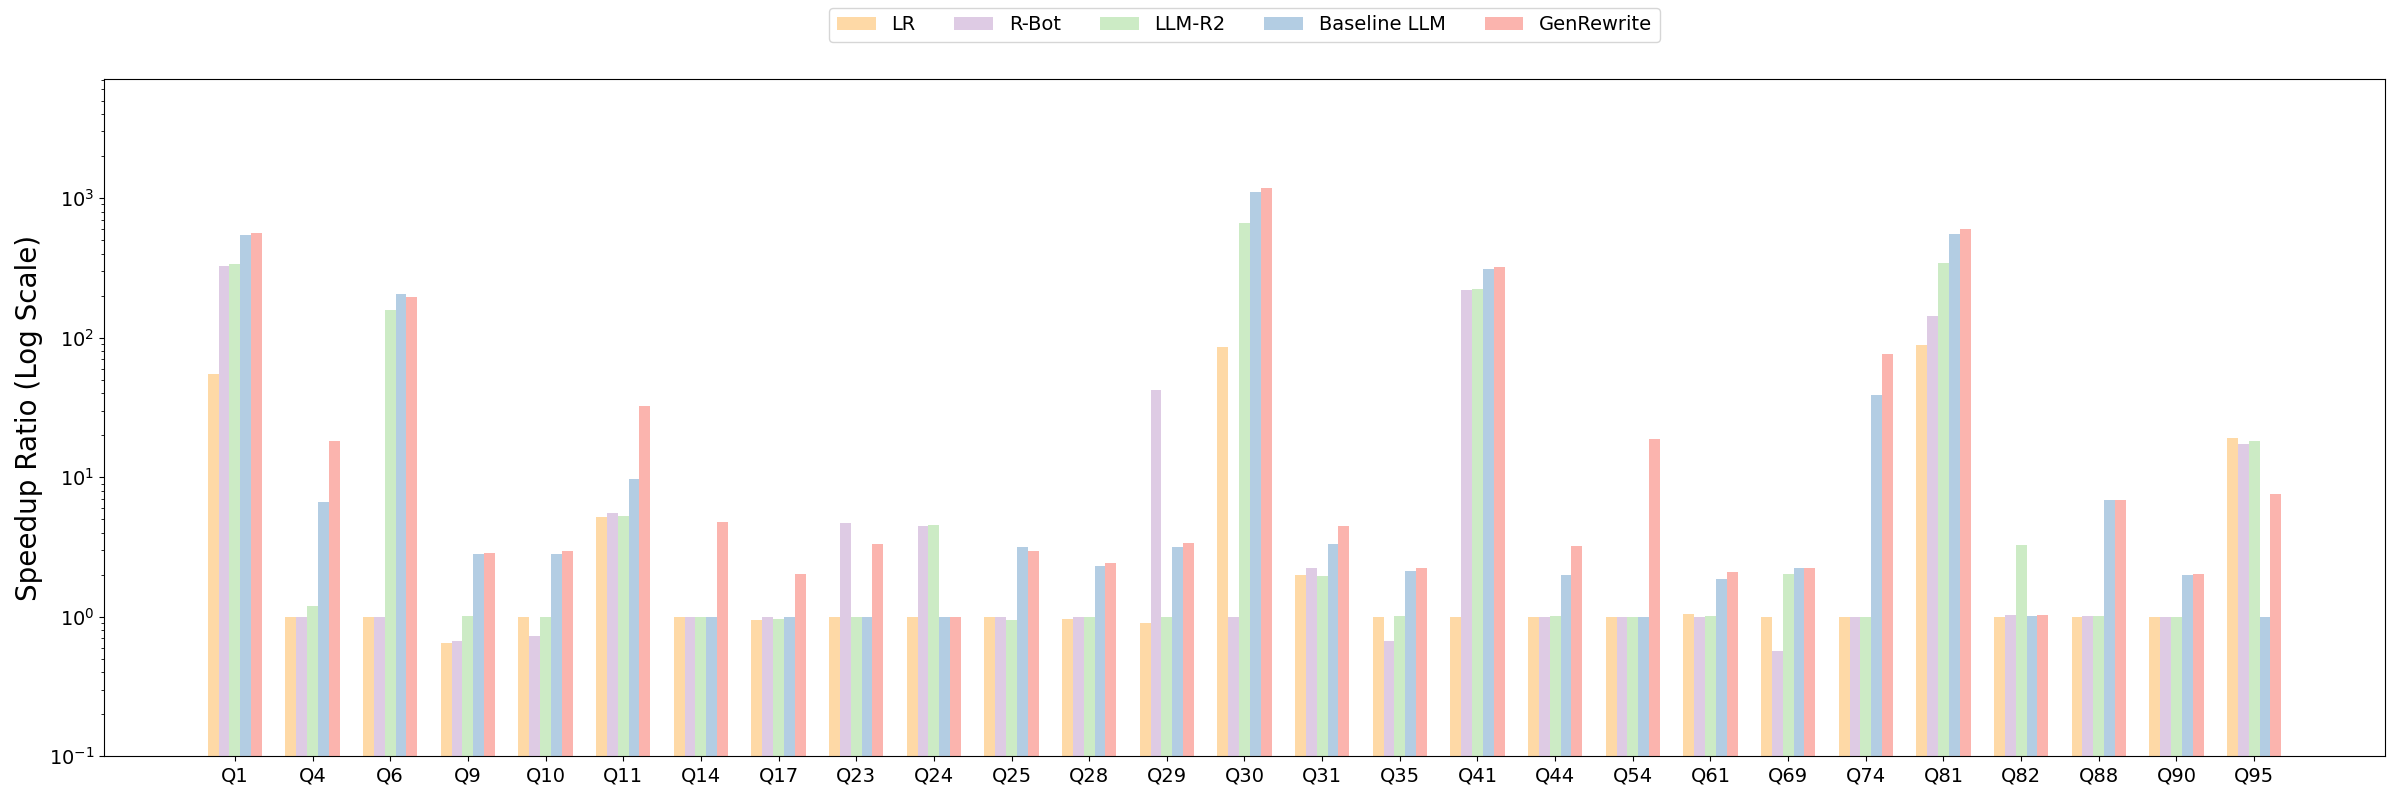
\includegraphics[width=\textwidth]{chapters/genrewrite/figures/baseline_comparison.png}
  \inv
  \vspace{-18pt}
  \captionsetup{font=small,name=Figure}
  \caption{Comparison of speedup achieved by different approaches on queries where at least one method attains a 2x or greater speedup. The y-axis is on a log scale.}
  \label{gen:fig:baseline}
  \inv
\end{figure*}

\end{comment}



\begin{comment}
    

In rule-based query rewriting, a set of pattern-matching rewrite rules define a fixed search space, resulting in consistent query outcomes across multiple runs. In contrast, due to the probabilistic nature of LLMs, 
    additional LLM runs increases the likelihood of uncovering new rewrite possibilities and thereby improving performance.
To ensure a fair comparison, we impose a limit on the number of LLM runs per query, 
    consistent with the setup outlined in Section~\ref{gen:sec:expr:llmbaseline}. Here, again, if a method fails to produce an equivalent rewrite for a particular query,  we deem the speedup ratio for that query as 1 indicating a fallback to the original query.
\end{comment}
% the number of iterations in \genrewrite to 5, including 4 i 
% a limit to the number LLM runs for each query in \genrewrite.

%  \genbarzan{check WA msg}
% \st{This predictability contrasts with the dynamic nature of LLM-based rewrites, where additional LLM runs increase the likelihood of uncovering new rewrite possibilities, potentially leading to significant performance boost.} 



% or if it is not applicable, \genbarzan{what does not applicable mean??}



\begin{comment}
    

\begin{table*}[h]
\centering
\begin{tabular}{lccccc}
\toprule
   & Syntax errors  & Semantic error & Regression (i.e., speedup < 1x) & >2x speedup \\
\midrule
\genrewrite & \textbf{4.3\%} &  \textbf{6.1\%}  & \textbf{2.0\%} & \textbf{21.2\%}  \\
Baseline LLM   & 30.3\%  & 29.3\% & 25.3\% & 10.1\% \\
\bottomrule
\end{tabular}
\caption{Comparison between \genrewrite and Baseline LLM on percentage of syntax error, syntax error, performance regression, more than 2x speedup}
\label{gen:tab:llmbaseline}
\end{table*}
\end{comment}


\subsection{Comparison with Rule-based Methods}
\label{gen:sec:expr:traditionalbaseline}


Analysis of Table.~\ref{gen:tab:speedup_all} shows that \genrewrite consistently surpasses the
three rule-based baselines in terms of the number of queries optimized, regardless of the desired speedup threshold, on all benchmarks. Other LLM-based methods also consistently outperform rule-based methods with smaller margins than \genrewrite.
We first consider the standard public benchmarks (Table~\ref{gen:tab:speedup_comparison}). On the original TPC-DS workload, \genrewrite identifies substantially more optimization opportunities than the rule-based baselines: it achieves at least 2x speedup on 25 queries, compared to 10, 9, and 6 queries for \textsc{LLM-R\textsuperscript{2}}, \rbot, and \lr, respectively. The advantage persists at higher thresholds (e.g., 10x speedup), and we observe a similar pattern on JOB. These results suggest that \genrewrite already outperforms established rule-based methods on well-studied public benchmarks.


\noindent\revtwo{SQLStorm workloads (Table~\ref{gen:tab:speedup_comparison_sqlstorm}) yield two key observations:}

\genhead{\revtwo{Observation 1}}
\revtwo{The performance gap between \genrewrite and the rule-based baselines widens on TPC-DS (SQLStorm).
    All three rule-based baselines (\textsc{LLM-R\textsuperscript{2}}, \rbot, and \lr) are built on top of Calcite and ultimately rely on Calcite’s rewrite rules. Their differences lie in rule selection and ordering, but they inherit the same two Calcite limitations: (1) \emph{Parser coverage:} The Calcite parser and validator do not fully support several constructs that appear in SQLStorm-generated  TPC-DS queries, such as recursive CTEs, \texttt{LENGTH}, etc. As a result, these systems only emit rewrites for roughly half of the input queries. (2) \emph{Rule coverage:} Even when Calcite can parse the query, its fixed rule set often fails to match the structure of these queries. SQLStorm's queries are not hand-polished benchmark SQL; they contain noisy nesting, ad hoc join predicates, and unseen operator combination that does not line up cleanly with Calcite’s stock transformations (e.g., predicate pushdown). In these cases, the systems may not show meaningful improvement. In contrast, \genrewrite does not depend on Calcite’s rule inventory. It can generate and iteratively refine rewrites for these same SQLStorm queries, which explains the widening gap on TPC-DS (SQLStorm).}

\genhead{\revtwo{Observation 2}}
\revtwo{On SQLStorm workloads, the ``LLM-enhanced'' rule-based systems degrade to the point that they can be outperformed by \lr, which does not use an LLM at all. \textsc{LLM-R\textsuperscript{2}} selects a few high-quality demonstration rewrites from a curated library using a learned retriever, and \rbot retrieves offline ``rewrite recipes'' mined from past queries. These strategies work on TPC-DS and JOB because the benchmark queries follow canonical patterns that are well represented in those demonstration pools. Under SQLStorm, however, the generated queries deviate substantially from those canonical patterns, so the retrieved demonstrations and recipes are often no longer relevant and provide poor guidance. \genrewrite, by contrast, is not limited to a static set of expert demonstrations or a fixed rule inventory. It employs iterative correction and accumulates transferable rewrite knowledge from prior queries, enabling it to adapt to new query forms without manual rule engineering.}



\revtwo{\genrewrite outperforms existing baselines both on the original TPC-DS / JOB benchmarks and on the SQLStorm-generated workloads. Its advantage becomes larger precisely in the regimes where fixed-rule systems provide poor coverage. If new rules were distilled from \genrewrite's successful rewrites on complex queries and then incorporated into Calcite, the rule-based methods could  be strengthened and extended to a broader class of queries.}



\genhead{\revtwo{A deeper look at rules discovered by \genrewrite}}
\revtwo{Besides standard Calcite rules (e.g., predicate pushdown, projection pruning), several papers propose more aggressive rewrite patterns for analytical workloads. Generalized Sub-Query Fusion~\cite{sarthi2020generalized} eliminates redundant I/O by fusing multiple similar subqueries into a single shared scan/aggregation. Super-operators~\cite{blitz2} collapse multi-branch aggregates and unions into a single streaming physical operator. The Spark engine in Azure Synapse~\cite{modi2021new} rewrites plans to reuse shuffles, push down filters and partial aggregates, and inject runtime partition pruning to reduce data movement. Athena~\cite{bruno2022computation} detects repeated expensive subplans in a query and fuses them so they are computed once and shared by all consumers. In Table~\ref{gen:tab:pattern-summary}, for each major rewrite pattern discovered by \genrewrite we ask: (1) does it align with any of these known patterns, at the idea level; and (2) is there an exact structural match already reported in prior work?}

% [leftmargin=0.5cm]

\noindent\revone{Representative optimization patterns discovered by \genrewrite:}
% \footnote{In Appendix~A, we present query pairs for each pattern and detail how they differ from prior work.}

\begin{enumerate}[leftmargin=0.5cm]
\item  \revone{Pivot with conditional aggregation instead of UNION-then-self-join.}
\item \revone{Replace multiple \texttt{EXISTS} conditions with a precomputed set via joins.}
\item \revone{Rewrite \texttt{COUNT(*)>0} as \texttt{EXISTS} (aggregate $\rightarrow$ semi-join; enables short-circuiting).}
\item \revone{Replace a bounded self-recursive CTE with a non-recursive base query \texttt{CROSS JOIN}ed to a small numbers table.}
\item \revone{Lift a per-key summary (e.g., item-level totals) into one CTE and drive all branches from it.}
\item \revone{Consolidate repetitive subqueries into a single aggregation subquery with conditional expressions.}
\item \revone{Decorrelate \texttt{IN} by joining a \texttt{SELECT DISTINCT} key,... mapping table instead of re-checking the subquery. }
\end{enumerate}


\begin{table}[tbp]
\inv
\small
\centering
\setlength{\tabcolsep}{6pt}
\def\arraystretch{1.2}

\begin{tabular}{ l | c c c }
\toprule
Pattern& Covered queries & Similar in idea & Exact match \\
\midrule
1 & 4, 11, 74 & ~\cite{blitz2}, ~\cite{bruno2022computation} & No \\
2 & 10, 35, 69 & ~\cite{begoli2018apache} & No \\
3 & 41 & ~\cite{begoli2018apache} & No \\
4 & 23998* &  & No \\
5 & 22722* & ~\cite{sarthi2020generalized}, ~\cite{bruno2022computation} & No \\
6 & 61, 88 & ~\cite{sarthi2020generalized}, ~\cite{bruno2022computation} & Yes,~\cite{bruno2022computation}  \\
7 & 28982*, 34389* & ~\cite{begoli2018apache} & Yes,~\cite{begoli2018apache}  \\
\bottomrule
\end{tabular}
\captionsetup{font=small,name=Table}
\caption{\revtwo{Summary of rewrite patterns discovered by \genrewrite. ``Covered queries'' lists the queries that exhibit each pattern (queries with * are from TPC-DS SQLStorm; others are from standard TPC-DS). ``Similar in idea'' notes prior work that proposes a conceptually related optimization. ``Exact match''indicates that the same structural rewrite has been reported before.}  }
\inv
\label{gen:tab:pattern-summary}
\end{table}











% \begin{enumerate}[leftmargin=0.5cm]

% \item  Pivot with conditional aggregation instead of UNION-then-self-join.
% \item Rewrite \texttt{COUNT(*)>0} as \texttt{EXISTS} (aggregate $\rightarrow$ semi-join; enables short-circuiting).
% \item Consolidate repetitive subqueries into a single aggregation subquery with conditional expressions.


% \end{enumerate}




\subsection{Detailed Analysis and Ablation Study}
\label{gen:sec:expr:ablation}

In this section, we conduct a detailed ablation study 
    to validate our design decisions in  \genrewrite and the contribution of each component therein towards the overall performance. We focus primarily on the \revtwo{original} TPC-DS benchmark, as its complexity provides a challenging test of our system's capabilities. The results, summarized in Table~\ref{gen:tab:ablation}, highlight the impact of individual components on LLM runtime overhead, monetary cost, and the percentage of queries achieving various levels of speedup.
    % To control for variables, we still adopt a setup in which our NLR2 repository is initialized with two LLM runs using the basic prompt and \genrewrite incorporates the NLR2 as a hint for the remaining two candidate rewrites,.


    




\begin{table*}[!t]
\small
\centering
\setlength{\tabcolsep}{5pt}
\def\arraystretch{1.1}
\vspace{-5pt}
\begin{tabular}{ | c | r r r r r |  }
\toprule
& \multicolumn{5}{c|}{TPC-DS} \\
 & >2x & >10x & >50x  & avg. time(s) & avg. cost(\$)  \\
\midrule
\genrewrite                           & \cntpct{25}{25.3} & \cntpct{9}{9.1}   & \cntpct{6}{6.1}   & 151.82 & 0.129 \\
\genrewrite without grouping NLR2s    & \cntpct{25}{25.3} & \cntpct{9}{9.1}   & \cntpct{6}{6.1}   & 385.47 & 0.310 \\
\genrewrite without bottleneck analysis & \cntpct{19}{19.2} & \cntpct{6}{6.1}   & \cntpct{5}{5.1}   & 150.30 & 0.124 \\
\genrewrite with gpt-4o               & \cntpct{14}{14.1} & \cntpct{5}{5.1}   & \cntpct{5}{5.1}   & 105.40 & 0.117 \\
\genrewrite with gpt-4-mini           & \cntpct{2}{2.0}   & \cntpct{1}{1.0}   & \cntpct{0}{0.0}   & 301.20 & 0.016 \\
\bottomrule
\end{tabular}
\captionsetup{font=small,name=Table}
\caption{Ablation study: impact of \genrewrite's design decisions on LLM runtime, cost, and the share of queries achieving various speedups.}
\label{gen:tab:ablation}
\vspace{-15pt}
\end{table*}



\genhead{Plan-based dominant NLR2 identification} This component plays a critical role in reducing query execution overhead, although its impact is not directly reflected in Table~\ref{gen:tab:ablation}. Without plan-based dominant NLR2 identification, we would need to execute each rewrite—generated by applying a single NLR2—to measure its runtime, which can be prohibitively expensive for long-running queries. 

\genhead{NLR2 grouping via LLM}
We collect an average of 5.08 NLR2s per input query after applying grouping, compared to 13.24 NLR2s per query without grouping. Although we only re-evaluate the impact of an NLR2 when the associated performance improvement exceeds a predefined threshold, grouping still significantly reduces both monetary and time costs. Without grouping, the average LLM runtime increases by 153.9\%, and the monetary cost rises by 140.3\%,  demonstrating that NLR2 grouping's impact on costs.


\genhead{Query performance bottleneck analysis} 
We compare two strategies: (1) apply the top NLR2s globally, ignoring query similarity; and (2) our default, which retrieves candidates by bottleneck similarity. The global strategy performs essentially the same as \baseline, indicating that ``best overall'' strategy rarely transfers. Bottleneck-aware retrieval, in contrast, delivers clear gains: effective reuse hinges on aligning NLR2s with performance bottlenecks.

% We evaluate two strategies for identifying queries with similar performance bottlenecks: (1) applying the top beneficial NLR2s regardless of query similarity, and (2) our default approach, which incorporates bottleneck-aware retrieval. Experimental results show that the first strategy performs nearly identically to \baseline, suggesting that indiscriminately applying high-performing NLR2s provides little benefit. This underscores the importance of relevance—effective reuse of NLR2s depends on accurately identifying queries with comparable performance bottlenecks.



\genhead{Choice of the LLM}
\genrewrite's performance critically depends on the LLM's reasoning capabilities. We evaluate three models: OpenAI’s \texttt{o3-mini} (reasoning-oriented), \texttt{gpt-4o} (balanced), and \texttt{gpt-4o-mini}(most cost-efficient).  \genrewrite powered by \texttt{gpt-4o} is noticeably outperformed by the \texttt{o3-mini} variant. We decompose \genrewrite’s workflow into two stages: (1) discovering effective rewrites and summarizing NLR2s, and (2) applying high-quality NLR2s to guide rewrites. We observe that \texttt{gpt-4o} struggles primarily in stage 1. However, when \genrewrite with \texttt{gpt-4o} is supplied with NLR2s previously discovered by \texttt{o3-mini}, the number of queries achieving a speedup $\geq$ 10× increases from 5 to 8,  further demonstrating the effectiveness of NLR2-guided rewriting.
% \texttt{gpt-4o-mini} rarely produces useful rewrites.



% \genrewrite’s gains track the model’s reasoning strength. \texttt{o3-mini} (reasoning-oriented) consistently finds stronger rewrites and better NLR2s, outperforming \texttt{gpt-4o}; \texttt{gpt-4o-mini} rarely produces useful rewrites. Decomposing \genrewrite into (i) discovery/summarization of NLR2s and (ii) application shows where the gap arises: \texttt{gpt-4o} underperforms in (i) but applies good NLR2s well—when seeded with \texttt{o3-mini}’s NLR2s, its count of >10× speedups rises from 5 to 8. Practical takeaway: use the strongest model for discovery, then a cheaper model can reliably apply the learned NLR2s.


\genhead{\revone{Parameter sensitivity analysis}}




\begin{table}[tbp]
\small
\centering
\begin{tabular}{l*{4}{cc}}
\toprule
& \multicolumn{2}{c}{$k{=}1$}
& \multicolumn{2}{c}{$k{=}2$}
& \multicolumn{2}{c}{$k{=}3$}
& \multicolumn{2}{c}{$k{=}4$} \\
\cmidrule(lr){2-3}
\cmidrule(lr){4-5}
\cmidrule(lr){6-7}
\cmidrule(lr){8-9}
& eq & fast
& eq & fast
& eq & fast
& eq & fast \\
\midrule
No correction
& 52 & 5
& 67 & 8
& 70 & 12
& 74 & 21 \\
Semantic only
& 54 & 5
& 68 & 10
& 71 & 14
& 75 & 21 \\
\textbf{Semantic + syntax}
& \textbf{70} & \textbf{5}
& \textbf{79} & \textbf{10}
& \textbf{85} & \textbf{16}
& \textbf{86} & \textbf{28} \\
\bottomrule
\end{tabular}
\captionsetup{font=small,name=Table}
\caption{\revone{Cumulative count of queries with (i) at least one equivalent rewrite (\textit{equiv}) and (ii) at least one equivalent rewrite that is at least 20\% faster than the original (\textit{faster}), as the candidate budget increases ($k{=}1\ldots4$), under different correction strategies.}}
\label{gen:tab:correction_ablation_new}
\inv
\end{table}


\noindent\revone{
\emph{\textbf{Budget:}} maximum candidates per query \(K=4\); correction caps \(I_{\mathrm{sem}}=I_{\mathrm{syn}}=3\) (semantic and syntax loops). For the TPC-DS workload, the average iterations is 0.30 (semantic) and 0.76 (syntax). The per-query correction iteration distributions are:}
\begin{itemize}
    \item \revone{Semantic: 0: 76.72\%, 1: 19.02\%, 2: 1.64\%, 3: 2.62\%.}
    \item \revone{Syntax: 0: 60.66\%, 1: 18.36\%, 2: 5.25\%, 3: 15.74\%.}
\end{itemize}
\revone{We vary the candidate budget $k \in\{1,2,3,4\}$. Table~\ref{gen:tab:correction_ablation_new} reports the \emph{cumulative} number of queries that achieve (i) $\geq 1$ equivalent rewrite and (ii) $\geq 1$ equivalent rewrite that is at least 20\% faster, as $k$ increases (higher \(k\) means more candidates attempted per input query), comparing: (i) no correction, (ii) semantic-only correction, and (iii) semantic\,+\,syntax correction.} \revone{Table~\ref{gen:tab:correction_ablation_new} shows that correction loops markedly reduce the effective error rate,  with \emph{semantic + syntax} outperforming the other settings at every \(k\). Larger \(k\) improves coverage with diminishing returns and proportionally higher cost.}


\noindent\revone{\emph{\textbf{Desired speedup threshold:}}
We set $\theta$ to 1.2x in our implementation. Increasing $\theta$ reduces coverage  but raises the average speedup among accepted rewrites. With a lower $\theta$, we keep more rewrites — including many that are only modestly better.}

\begin{table}[H]
\small
\centering
\begin{tabular}{lccc}
\toprule
Desired speedup threshold $\theta$ & 1.2x & 2.0x & 5.0x \\
\midrule
Coverage (\%)       & 28.3 & 23.2 & 13.1 \\
Geom.\ mean speedup & 11.1x & 17.0x & 72.2x \\
\bottomrule
\end{tabular}
\captionsetup{font=small,name=Table}
\caption{\revone{Coverage and geometric mean speedup for desirable speedup thresholds $\theta \in \{1.2x,1.5x,2.0x\}$. 
Coverage(\%) is the fraction of queries with $\ge\theta$ speedup; geom.\ mean is over covered queries.}}
\label{gen:tab:theta_sweep}
\inv
\end{table}

\vspace{-5mm}

\genhead{\revthree{Counterexample-guided iterative correction}} 
\revthree{We compare our counterexample-based semantic check to Miniature \& Mull from LLM-SQL-Solver~\cite{zhao2023llm} on random TPC-DS rewrites (no correction). Our prompt yields 29\% equivalent rewrites before syntax correction with a 6\% false-positive rate; Miniature \& Mull achieves 26\% equivalents with 22\% false positives. Thus our prompt better aligns with the iterative correction task—more verified equivalents and far fewer false positives.}



% \revthree{LLM-SQL-Solver~\cite{zhao2023llm} introduces the Miniature \& Mull prompting strategy for equivalence checking, which also searches for counterexamples and bases the decision on them. For a head-to-head comparison, we replaced our semantic-checking prompt with theirs and evaluated both settings on randomly sampled TPC-DS rewrites without any correction. With our prompt—which asks the LLM to produce a concrete counterexample and then feeds it back as a hint for semantic correction—we obtain 29\% equivalent rewrites \emph{before} syntax correction stage and a 6\% false-positive rate (inequivalent rewrites judged equivalent). Using Miniature \& Mull, we observe 26\% equivalent rewrites and a 22\% false-positive rate under the same protocol. This indicates our semantic-checking prompt is better aligned with the rewrite-correction loop, yielding more verified equivalents while substantially reducing false positives.}


% LLM-SQL-Solver proposes Miniature and Mull prompting technique for equivalence checking, which shares similar idea with our method about finding counterexamples and then give the conclusion. We replace our semantic checking prompt with theirs and test both on TPC-DS workloads. The result shows that with our semantic checking prompt which asks for a counterexample from LLMs and then be used as the hints for semantic corrections, we get 29\% equivalent queries (before syntax correction) and 6\%  false positive (LLMs consider the inequivalent rewrites to be equivalent). For LLM-SQL-Solver, we get 26\% equivalent queries and 22\% false positives. Our semantic checking prompt suits better with this rewrite correction task.














\begin{comment}


\genhead{Impact of semantic   and syntax correction} For each TPC-DS query, we conduct 4 independent runs to generate 4 candidate rewrites. In each run, we use zero-shot prompting (Baseline LLM) to suggest candidate queries and adopt one of the following correction strategies before assessing the correctness and performance of the rewrite.

\begin{enumerate}
    \item No correction.
    \item Only semantic correction.
    \item Only syntactic correction.
    \item Two-stage correction (semantic correction and then syntax correction).
\end{enumerate}



\noindent We set the maximum iteration count 3 for both semantic and syntax correction.

Table~\ref{gen:tab:correction_ablation} compares cumulative equivalent rewrites generated by various correction strategies over successive runs, with each cell showing the number of TPC-DS queries equivalently rewritten by a specific strategy up to that point (the highest possible is 99). The analysis clearly demonstrates that the two-stage correction strategy outperforms others, and not applying any correction yields the least effective results, with the remaining strategies falling in between. In a direct comparison between ``Only semantic correction'' and ``Only syntax correction'', the latter shows a quicker ability to produce executable and equivalent rewrites for simpler queries in the first few runs. However, its effectiveness is limited by a lower ceiling due to a lack of understanding regarding the queries' intent, leading to executable but inequivalent rewrites for more complex queries. When combining these two strategies together, semantic correction interprets the intent, ensuring the rewrite's objectives align with the original query, and then syntax correction refines the rewrite to be executable. The two-stage strategy (i.e., semantic + syntax) identifies equivalent rewrites for 70 of the 99 TPC-DS queries in the first run. It then adds 3 more in the second run and 6 in the third, ultimately achieving equivalent rewrites for 90 of the 99 queries.



\begin{table}[h]
\centering
\begin{tabular}{lcccc}
\toprule
 & run 1 & run 2 & run 3 & run 4 \\
\midrule
No correction & 45 & 56 & 65 & 69  \\
Only semantic & 51 & 66 & 76 & 82 \\
Only syntactic & 60 & 68 & 73 & 76 \\
\textbf{Semantic + syntactic} & \textbf{70} & \textbf{81} & \textbf{87} & \textbf{90} \\
\bottomrule
\end{tabular}
\caption{Cumulative count of equivalent rewrites   using different correction strategies over multiple runs.}
\label{gen:tab:correction_ablation}
\inv
\end{table}



Delving deeper into the two-stage correction strategy, it generally achieves convergence quickly, usually within 3 iterations, except for a small number of cases involving overly complex queries. However, there is still a gap between the queries deemed equivalent by the LLM and those that are truly equivalent. The non-cumulative count of queries  verified as equivalent in each run are 69, 75, 69, and 70, respectively.  When aggregating results from all runs, 90 unique queries are   equivalent, indicating that the sets of queries identified as equivalent in each run vary.




    

\genhead{Impact of NLR2s as hints}  After conducting 4 rounds of zero-shot prompting, we reach a stable state where additional rounds fail to bring improvements in terms of the number of rewrites that are both equivalent and faster.
This suggests that we effectively capture most of low-hanging fruits. A comparative analysis between an additional iteration using zero-shot prompting and another leveraging prompts augmented with specific NLR2 hints reveals a pronounced superiority of the latter. The queries solvable exclusively through hint-augmented prompts 
are presented in Table~\ref{gen:tab:knowledge_ablation}.


% Two crucial observations are highlighted in Section 3: LLMs are more likely to struggle in identifying rewrite opportunities with increasing query complexity; LLMs can optimize queries that they previously struggled to optimize when provided with suitable hints in the prompt. The primary goal of employing NLR2s is to facilitate knowledge transfer and bridge the gap between queries that LLMs can optimize without hints and those they cannot, enabling LLMs to optimize a broader range of queries.

% \begin{table}[ht]
% \centering
% \caption{Rewrite hints .}
% \label{gen:tab:knowledge_ablation}
% \begin{tabular}{lccccc}
% \toprule
%  & Q4 & Q11 & Q20 & Q29 & Q76 \\
% \midrule
% Without hints & - & 1.07x & 1x & 1.42x & 1x  \\
% With hints & \textbf{5.68x} & \textbf{10.3x} & \textbf{9.89x} & \textbf{6.85x} & \textbf{9.77x} \\
% \bottomrule
% \end{tabular}
% \end{table}


% \begin{table}[h]
% \centering
% \caption{NLR2s inspired speedups}
% \label{gen:tab:knowledge_ablation}
% \begin{tabular}{ccc p{4cm}}
% \toprule
% input & speedup & inspired by & \small{NLR2s} \\
% \hline
% 4 & 5.68x & 74 &  \footnotesize{Avoid UNION ALL if not necessary \newline Split complex queries into simpler ones using WITH clause} \\ \hline
% 11 & 10.3x & 74 & \footnotesize{Avoid UNION ALL if not necessary \newline Split complex queries into simpler ones using WITH clause} \\ \hline
% 20 & 9.89x & 12 &  \footnotesize{Use CTE (Common Table Expressions) to break down complex queries \newline Reduce the number of tables in the join operation} \\ \hline
% 29 & 6.85x & 25 &  \footnotesize{Aggregate before join \newline Use subqueries to break down complex queries} \\ \hline
% 76 & 9.77x & 61 &  \footnotesize{Combine multiple queries into a single query \newline Move WHERE clause filters to ON clause in JOINs} \\
% \bottomrule
% \end{tabular}
% \end{table}





Q4, Q11, and Q74 all see improvements by eliminating the unnecessary \sqlunionallcolor, which has been discussed in earlier sections. Q20 benefits from NLR2s learned from its neighboring query Q12. Inspired by the rule ``Use CTE to break down complex queries'', the actual transformation applied is a group-by pushdown. Q29 is solved using similar ideas but exhibits a different query pattern and learns from Q25.
For Q76,  where multiple segments each join two common tables across several subqueries, the rewrite strategy is to combine these segments with \sqlunionallcolor before conducting a join with the common tables, thereby avoiding duplicate computation. This strategy is inspired by the rule ``Combine multiple queries into one query'' from Q61. These instances underscore the value of employing NLR2s for effective knowledge transfer across queries. At the conclusion of our experiments, we collect 156 groups of rewrite rules,  with an average of 7 rules per group.
\end{comment}

\begin{comment}
    

\genhead{\texttt{EXPLAIN} cost vs. actual latency} When evaluating rewrites, we can either utilize the database's own cost estimates as a surrogate for actual performance (i.e., using \texttt{EXPLAIN}) 
or measure the latency by actually running candidate queries directly on the database or a small sample of it. The latter approach, while offering greater accuracy, also results in higher costs, which is justifiable when the query is optimized once and rewritten many times (see target use case in \S\ref{gen:sec:intro}). The goal of this experiment is to quantify the negative impact of using 
inaccurate cost estimates on \genrewrite's performance.

We examine two variants of \genrewrite, differing only in their choice of evaluation metric. One variant calculates the utility scores of NLR2s   based on actual latency while the other relies on \texttt{EXPLAIN}'s cost estimates. 
The comparison between the two variants is detailed in 
Table~\ref{gen:tab:latency_vs_cost}. We observe that both coverage and latency reduction ratios are lower when \texttt{EXPLAIN} is used for query evaluation. This is expected: (1) cost estimates do not accurately reflect actual latency, meaning a rewrite with a lower cost estimate does not guarantee lower latency; (2) the speedup ratios derived from cost estimates can be disproportionately high, not aligning with the actual latency improvements, thereby impacting the effectiveness of NLR2s. Despite these issues, the variant that rely on \texttt{EXPLAIN} cost still outperforms all other baselines.

\end{comment}








\subsection{Time and Monetary Cost}
% \subsection{Cost analysis of LLM}
\label{gen:sec:expr:llmcost}


While \genrewrite’s time and API costs are a one-time, amortized expense for recurring workloads (see Target workloads in \S\ref{gen:sec:intro}), we still quantify them to ensure they remain modest. Using OpenAI’s \texttt{o3-mini} to generate a rewrite for a TPC-DS query—including suggestion, semantic correction, and syntactic correction—costs on average \$0.029 and takes 36.15 s. For comparison, \texttt{gpt-4o} and \texttt{gpt-4o-mini} average (\$0.026, 25.1 s) and (\$0.004, 71.71 s), respectively. As a reasoning-focused model, \texttt{o3-mini} consumes more tokens, increasing cost but often yielding more logically sound, well-structured rewrites for complex SQL transformations. Auxiliary LLM steps (e.g., grouping NLR2s and selecting the bottleneck) add negligible overhead. Overall, total cost scales approximately linearly with the number of candidate rewrites generated by the pipeline.


%  Although the time and monetary cost of \genrewrite is not as relevant given that it is a one-time cost that gets amortized for recurrent workloads (see Target workloads in \S\ref{gen:sec:intro}), we still need to ensure they do not become excessive.
% Using OpenAI’s \texttt{o3-mini} model to generate a rewrite for a TPC-DS query—including rewrite suggestion, semantic correction, and syntactic correction—incurs an average cost of approximately \$0.029 and takes 36.15 seconds. For comparison, \texttt{gpt-4o} and \texttt{gpt-4o-mini} yield average costs and durations of (\$0.026, 25.1 seconds) and (\$0.004, 71.71 seconds), respectively. \texttt{o3-mini}, being a reasoning-focused model, tends to consume significantly more tokens during generation. While this leads to higher total costs, the increased token usage contributes to more logically sound and well-structured rewrites, especially in the context of complex SQL transformation tasks.
% The cost associated with auxiliary LLM tasks, such as grouping NLR2s and selecting the most relevant bottleneck  is negligible in practice. Overall, the total cost of the system grows linearly with the number of candidates generated with the rewriting pipeline.


% Although \texttt{gpt-4o} is approximately twice as expensive per token as \texttt{o3-mini}, and roughly 16 times more expensive than \texttt{gpt-4o-mini}, our experiments show that the overall cost of using \texttt{o3-mini} is actually higher than that of \texttt{gpt-4o}. This counterintuitive result stems from the fact that \texttt{o3-mini}, being a reasoning-focused model, tends to consume significantly more tokens during generation. While this leads to higher total costs, the increased token usage contributes to more logically sound and well-structured rewrites, especially in the context of complex SQL transformation tasks.
% The cost associated with auxiliary LLM tasks, such as grouping NLR2s and selecting the most relevant bottleneck from the top-$k$ candidates—is negligible in practice. Overall, the total cost of the system grows linearly with the number of iterations of the rewriting pipeline.



\begin{table}[h]
% \small
\footnotesize
\centering
\setlength{\tabcolsep}{6pt}
\def\arraystretch{1.1}
\vspace{-5pt}
\begin{tabular}{  c | r r r | r r r }
\toprule
& \multicolumn{3}{c|}{time (s)} 
& \multicolumn{3}{c}{monetary cost (\$)} \\
stage & suggest & \makecell{semantic\\corr.} & \makecell{syntax\\corr.} & suggest & \makecell{semantic\\corr.} & \makecell{syntax\\corr.} \\
\midrule
o3-mini     & \makecell{5.8\\(16.0\%)} & \makecell{20.8\\(57.6\%)}  & \makecell{9.6\\(26.5\%)}  & \makecell{7.8e-03\\(26.4\%)} & \makecell{1.5e-02\\(52.2\%)}  & \makecell{6.3e-03\\(21.3\%)} \\
gpt-4o & \makecell{1.5\\(5.8\%)} & \makecell{22.1\\(87.9\%)}  & \makecell{1.6\\(6.3\%)}  & \makecell{6.4e-03\\(23.9\%)} & \makecell{1.9e-02\\(70.1\%)}  & \makecell{1.6e-03\\(6.0\%)} \\
gpt-4o-mini & \makecell{1.9\\(2.6\%)} & \makecell{66.8\\(93.1\%)}  & \makecell{3.1\\(4.3\%)}  & \makecell{4.0e-04\\(11.2\%)}  & \makecell{3.1e-03\\(84.6\%)}   & \makecell{1.5e-04\\(4.2\%)} \\
% \rbot       & \makecell{9\\(9.1\%)}  & \makecell{5\\(5.1\%)}   & \makecell{3\\(3.0\%)}   & \makecell{7\\(6.2\%)}  & \makecell{3\\(2.7\%)}   & \makecell{2\\(1.8\%)} \\
% \lr       & \makecell{6\\(6.1\%)}  & \makecell{4\\(4.0\%)}   & \makecell{0\\(0\%)}   & \makecell{6\\(5.3\%)}  & \makecell{2\\(1.8\%)}   & \makecell{1\\(0.9\%)} \\
\bottomrule
\end{tabular}
\captionsetup{font=small,name=Table}
\caption{\small LLM cost analysis: the monetary and time cost of generating one rewrite candidate for a TPC-DS query, including all three stages--- rewrite suggestions, semantic correction, and syntactic correction.}
\inv
\label{gen:tab:llm_cost}
\vspace{-10pt}
\end{table}

 
 % The breakdown of the monetary and time cost is presented in Table~\ref{gen:tab:llm_cost}. Across all three models, semantic correction phase accounts for the highest cost in terms of both monetary and time cost. However, when using \texttt{o3-mini}, a larger portion of time is also spent on the candidate suggestion and syntax correction phases. This is because \texttt{o3-mini}, with its stronger reasoning capabilities, tends to better understand the input query and generate more aggressive rewrites. While this increases the likelihood of discovering high-quality transformations, it also lowers the chance of producing equivalent rewrites on the first attempt, thereby requiring additional iterations in the syntax correction phase. In contrast, the two lower-capacity models exhibit a more conservative rewriting style, leading to fewer iterations but also fewer opportunities for substantial performance improvement.

 Table~\ref{gen:tab:llm_cost} shows that semantic correction dominates both time and cost across models. With \texttt{o3-mini}, more time also goes to candidate suggestion and syntax correction: its stronger reasoning yields more aggressive rewrites (more chances for big wins) but requires extra iterations to ensure equivalence. By contrast, \texttt{gpt-4o} and \texttt{gpt-4o-mini} rewrite more conservatively, needing fewer iterations but offering fewer opportunities for substantial speedups.

\revone{For equivalence checking, we set a 60 sec timeout for the tester and 5 sec for the verifier. Performance–evaluation time varied by query from seconds to hours. We also terminated execution early when a candidate failed to exceed the original query by the desired speedup threshold $\theta$.}

 


% \subsection{Choice of the LLM}
% \label{gen:sec:expr:llmchoice}

% The performance of components in \genrewrite critically depends on the knowledge and reasoning capabilities of the chosen LLM. If an LLM fails to optimize queries, no transferable knowledge is generated, and if it does not accurately capture a query’s objective, it is unlikely to identify relevant counterexamples. We evaluate three LLMs with varying costs and capabilities: OPENAI o3-mini, which excels at reasoning; gpt-4, the state-of-the-art general-purpose model; and gpt-3.5-turbo, which provides basic text understanding. As shown in Table~\ref{gen:tab:ablation}, OPENAI o3-mini achieves the best speedup statistics at a modest cost, demonstrating both the rapid progress in language models for complex tasks and the powerful reasoning capabilities even in small-scale models.





% \genhead{LLM's capacity}






% evaluating queries with explain costs or actual latency


% \noindent\textbf{Compared approaches.} To understand the contribution of various components within our tool, we remove certain components to compare its performance with that of the complete tool.

% \begin{itemize}
%     \item \textbf{Zero-shot prompts with no correction.}
%     \item \textbf{Zero-shot prompts with only semantic correction.}
%     \item \textbf{Zero-shot prompts with only syntax correction.}
%     \item \textbf{Zero-shot prompts with two-stage correction.}
%     \item \textbf{Prompts with rewrite hints (\texttt{EXPLAIN} cost).}
%     \item \textbf{Prompts with rewrite hints (actual latency).}
%     \item \textbf{}
%     \item 
    
% \end{itemize}



\begin{comment}
    
\begin{table}[!t]
\small
\centering
\setlength{\tabcolsep}{6pt}
\def\arraystretch{1.1}

\vspace{-5pt}
\begin{tabular}{  c | r r r | r r r }
\toprule
& \multicolumn{3}{c|}{TPC-DS} 
& \multicolumn{3}{c}{JOB} 
%& \multicolumn{2}{c|}{TPC-H} 
%& \multicolumn{2}{c}{TPC-DS} 
\\ 
speedup & >2x 
& >10x
& >50x 
& >1.2x 
& >2x
& >10x 
%& median 
%& max 
%& median 
%& max 
\\ 
\midrule
\genrewrite
& {25} & {9} & 
 {6}	&  {24}	& 8
& 3 
 %& \ruirevisiontbd{4.15}  &  \ruirevisiontbd{4.58}	 &  \ruirevisiontbd{5.03}		& \ruirevisiontbd{5.74}
\\ 
\baseline
& 18 & 6 & 5	& 19	 & 7
& 3 
%& 0.25 & 	1.58 & 	2.48	& 25.51 
\\ 
\textbf{LLM-R\textsuperscript{2}}
& 10	& 6 &	5	& 9	& 2
& 1 
%& 0.36	& 0.36	& NA &	NA 
\\ 
\lr
& 6	& 4 &	0	& 6	& 2
& 1
%& 0.36	& 0.36	& NA &	NA 
\\ 

\bottomrule
\end{tabular}
\caption{\small Speedup.}
\label{gen:tab:f}
\vspace{-15pt}
\end{table}
\end{comment}



\begin{comment}
    Since LLMs operate probabilistically, more trials increase the chances of finding a better rewrite. However, this is impractical due to time and cost constraints. Therefore, a system that more effectively uncovers hidden rewrite opportunities can significantly reduce both computational expenses and execution time.

From Table~\ref{gen:speedup_comparison}, we could see that both LLM-based 
which could be easily explained as LLMs have accumulated a solid knowledge base from the massive training data

\end{comment}


\begin{comment}
     Table~\ref{gen:tab:llmbaseline} shows a direct comparison between \genrewrite and  Baseline LLM. 
Notably, 30.3\% of  Baseline LLM's rewrites  are unexecutable (due to syntax error), compared to only 4.3\% for \genrewrite. The percentage of rewrites leading to semantic errors (i.e., non-equivalent rewrites) for Baseline LLM is 29.3\%, compared to only 6.1\% for \genrewrite. Both results demonstrate the effectiveness of our iterative correction strategy.


%marginally higher than BaselineLLM's 18.7\%, a result that initially appears surprising. In fact, it does not imply that \genrewrite's syntax correction is useful while its semantic correction is flawed. An unexecutable rewrite may indicate either a syntax error or both syntax and semantic errors, meaning SemanE does not accurately capture the ratio of semantic errors. A significant portion of SynE also has semantic errors.

\genrewrite results in only 2 performance regressions from 93 queries with equivalent rewrites-—-defined as those with over 5\% longer execution time than the original query--—while Baseline LLM experiences 23 performance regressions out of 70 equivalent rewrites. Moreover, \genrewrite achieves more than a 2x speedup in its rewrites twice as often as Baseline LLM. There two statistics show the effectiveness of our knowledge transfer.

% \genrewrite has a 25\% chance of generating incorrect queries, significantly lower than Baseline LLM's 49\%. Consequently, \genrewrite can produce equivalent rewrites for 93.9\% of TPC-DS queries, compared to Baseline LLM's 70.7\%. When selecting the best rewrites for comparison with the input queries, 

Overall, these results show the effectiveness of \genrewrite in drastically improving the quantity and quality of rewrites that one can achieve by na\"ively invoking the LLM.


Separate evaluation of NLR2s not only identify the exact contribution of each NLR2 but also find the NLR2 that leads to inequivalence. For example

\end{comment}


\begin{comment}
    
\begin{table}[tb]
\centering
\begin{tabular}{lccccc}
\toprule
speedup & >10\% & >50\% & >2x & >10x & >100x \\
\midrule
Using latency & \textbf{33.3\%} & \textbf{24.2\%} & \textbf{21.2\%} & \textbf{9.1\%} & \textbf{3.0\%} \\
Using \texttt{EXPLAIN} cost & 23.2\% & 16.2\% & 13.1\% & 7.1\% & \textbf{3.0\%} \\
\bottomrule
\end{tabular}
\caption{Comparison of the percentage of queries optimized when using latency and \texttt{EXPLAIN} cost as the evaluation metric}
\label{gen:tab:latency_vs_cost}
\inv
\end{table}
\end{comment}



\begin{comment}
    \begin{table}[tb]
\inv
\centering
\setlength{\tabcolsep}{3pt} % Adjust the space between columns
\begin{tabular}{@{}cccp{4.5cm}@{}}
\toprule
input & speedup & inspired by & \small{NLR2s} \\
\midrule
Q4 & 5.68x & Q74 &  \footnotesize{Avoid UNION ALL if not necessary; \newline Split complex queries into simpler ones using WITH clause} \\
Q11 & 10.3x & Q74 & \footnotesize{Avoid UNION ALL if not necessary; \newline Split complex queries into simpler ones using WITH clause} \\
Q20 & 9.89x & Q12 &  \footnotesize{Use CTE (Common Table Expressions) to break down complex queries; \newline Reduce the number of tables in the join operation} \\
Q29 & 6.85x & Q25 &  \footnotesize{Aggregate before join; \newline Use subqueries to break down complex queries} \\
Q76 & 9.77x & Q61 &  \footnotesize{Combine multiple queries into a single query; \newline Move WHERE clause filters to ON clause in JOINs} \\
\bottomrule
\end{tabular}
\caption{NLR2s inspired speedups}
\label{gen:tab:knowledge_ablation}
\inv
\end{table}
\end{comment}


\begin{comment}
    \begin{table}[H]
\small
\centering
\begin{tabular}{lcccc}
\toprule
 & \(k{=}1\) & \(k{=}2\) & \(k{=}3\) & \(k{=}4\) \\
\midrule
No correction & 52 & 67 & 70 & 74 \\
Semantic only & 54 & 68 & 71 & 75 \\
\textbf{Semantic + syntax} & \textbf{70} & \textbf{79} & \textbf{85} & \textbf{86} \\
\bottomrule
\end{tabular}
\captionsetup{font=small,name=Table}
\caption{Cumulative count of queries with $\geq$1 equivalent rewrites as the candidate budget increases (\(k=1\ldots 4\)), under different correction strategies.}
\label{gen:tab:correction_ablation}
\inv
\end{table}
\end{comment}




\begin{comment}


\begin{table}[H]
\small
\centering
\setlength{\tabcolsep}{6pt}
\def\arraystretch{1.1}
\vspace{-5pt}
\begin{tabular}{  c | r r r | r r r }
\toprule
& \multicolumn{3}{c|}{TPC-DS} 
& \multicolumn{3}{c}{JOB} \\
speedup & >2x & >10x & >50x & >1.2x & >2x & >10x \\
\midrule
\genrewrite     & \makecell{25\\(25.3\%)} & \makecell{9\\(9.1\%)}  & \makecell{6\\(6.1\%)}  & \makecell{20\\(17.7\%)} & \makecell{8\\(7.1\%)}  & \makecell{3\\(2.7\%)} \\
\baseline & \makecell{18\\(18.2\%)} & \makecell{6\\(6.1\%)}  & \makecell{5\\(5.1\%)}  & \makecell{19\\(16.9\%)} & \makecell{7\\(6.2\%)}  & \makecell{3\\(2.7\%)} \\
\lithe & \makecell{16\\(x\%)} & \makecell{6\\(6.1\%)}  & \makecell{4\\(x\%)}  & \makecell{17\\(x\%)} & \makecell{6\\(x\%)}  & \makecell{1\\(x\%)} \\
\textsc{LLM-R\textsuperscript{2}} & \makecell{10\\(10.1\%)} & \makecell{6\\(6.1\%)}  & \makecell{5\\(5.1\%)}  & \makecell{9\\(8.0\%)}  & \makecell{2\\(1.8\%)}   & \makecell{1\\(0.9\%)} \\
\rbot       & \makecell{9\\(9.1\%)}  & \makecell{5\\(5.1\%)}   & \makecell{3\\(3.0\%)}   & \makecell{7\\(6.2\%)}  & \makecell{3\\(2.7\%)}   & \makecell{2\\(1.8\%)} \\
\lr       & \makecell{6\\(6.1\%)}  & \makecell{4\\(4.0\%)}   & \makecell{0\\(0\%)}   & \makecell{6\\(5.3\%)}  & \makecell{2\\(1.8\%)}   & \makecell{1\\(0.9\%)} \\
\bottomrule
\end{tabular}
\captionsetup{font=small,name=Table}
\caption{Speedup Comparison between all methods on original TPCDS and JOB workloads.}
\label{gen:tab:speedup_comparison}
\vspace{-15pt}
\end{table}



\begin{table}[H]
\small
\centering
\setlength{\tabcolsep}{6pt}
\def\arraystretch{1.1}
\vspace{-5pt}
\begin{tabular}{  c | r r r | r r r }
\toprule
& \multicolumn{3}{c|}{TPC-DS (SQLStorm)} 
& \multicolumn{3}{c}{JOB (SQLStorm)} \\
speedup & >2x & >10x & >50x & >1.2x & >2x & >10x \\
\midrule
\genrewrite     & \makecell{25\\(25.3\%)} & \makecell{9\\(9.1\%)}  & \makecell{6\\(6.1\%)}  & \makecell{20\\(17.7\%)} & \makecell{8\\(7.1\%)}  & \makecell{3\\(2.7\%)} \\
\baseline & \makecell{18\\(18.2\%)} & \makecell{6\\(6.1\%)}  & \makecell{5\\(5.1\%)}  & \makecell{19\\(16.9\%)} & \makecell{7\\(6.2\%)}  & \makecell{3\\(2.7\%)} \\
\lithe & \makecell{16\\(x\%)} & \makecell{6\\(6.1\%)}  & \makecell{4\\(x\%)}  & \makecell{17\\(x\%)} & \makecell{6\\(x\%)}  & \makecell{1\\(x\%)} \\
\textsc{LLM-R\textsuperscript{2}} & \makecell{10\\(10.1\%)} & \makecell{6\\(6.1\%)}  & \makecell{5\\(5.1\%)}  & \makecell{9\\(8.0\%)}  & \makecell{2\\(1.8\%)}   & \makecell{1\\(0.9\%)} \\
\rbot       & \makecell{9\\(9.1\%)}  & \makecell{5\\(5.1\%)}   & \makecell{3\\(3.0\%)}   & \makecell{7\\(6.2\%)}  & \makecell{3\\(2.7\%)}   & \makecell{2\\(1.8\%)} \\
\lr       & \makecell{6\\(6.1\%)}  & \makecell{4\\(4.0\%)}   & \makecell{0\\(0\%)}   & \makecell{6\\(5.3\%)}  & \makecell{2\\(1.8\%)}   & \makecell{1\\(0.9\%)} \\
\bottomrule
\end{tabular}
\captionsetup{font=small,name=Table}
\caption{Speedup Comparison between all methods on original TPCDS and JOB workloads.}
\label{gen:tab:speedup_comparison_sqlstorm}
\vspace{-15pt}
\end{table}
    
\end{comment}


\begin{comment}

\item \textbf{TPC-DS} is a widely recognized, industry-standard decision support benchmark.
% , which is designed to provide relevant, objective performance data to industry users
 Even though
TPC-DS may not perfectly model the recurring workloads seen in production environments, it still serves as a valuable reference for assessing the efficacy of different query rewriting techniques on complex, real-life queries. We generated 
a 10GB TPC-DS dataset and considered all of the 99 queries in the benchmark. 

\item \textbf{JOB}~\cite{leis2015good} which is based on the IMDB data set, is a widely adopted test suite used to evaluate query optimization strategies in relational database systems. It consists of queries with varying degrees of complexity and multiple join operations, reflecting realistic workloads.

\item \textbf{TPC-DS (SQLStorm)} SQLStorm generates tens of thousands of queries using TPC-DS schema. Since calling LLM API incurs cost, it is not practical to test against all of them. We selected top 100 queries having the longest running time when testing using olapbench. All of the selected queries are of medium to high complexity based on SQLStorm's analysis.

\item \textbf{JOB (SQLStorm)} Similar to TPC-DS (SQLStorm), we also selected top 50 queries having the longest running time when testing using olapbench. All of the selected queries are of medium to high complexity based on SQLStorm's analysis.

    
\end{comment}


\begin{comment}

\revone{Table~\ref{gen:tab:speedup_all} presents the speedup comparison beween all methods. Before going into details, note that no matter it is the original workloads or SQLStorm-generated variants, queries in the JOB benchmark tend to be less complex compared to TPC-DS. First, the average query length in JOB is 278.81 tokens, while TPC-DS queries average 441.34 tokens—a 58\% increase. Second, although JOB queries can involve many joins and may present a combinatorial challenge in terms of finding the optimal join sequence, their structural complexity is lower: they feature fewer nested subqueries, window functions, and set operations than TPC-DS queries. When SQLStorm generates queries for TPC-DS and JOB schemas, JOB queries are still limited by the relatively narrow and normalized tables and lack of comparisons across channels or time windows } 
    
\end{comment}


% or if it is not applicable, \genbarzan{what does not applicable even mean?}


% \genrewrite & \textbf{4.3\%} &  \textbf{6.1\%}  & \textbf{2.0\%} & \textbf{21.2\%}  \\
% Baseline LLM   & 30.3\%  & 29.3\% & 25.3\% & 10.1\% \\

% Both \genrewrite and \baseline are given four attempts to propose candidate rewrites for each input query. 

% Table.~\ref{gen:tab:speedup_all} reports the percentage by dividing the number of queries by the total number of input queries, 99 for TPC-DS and 113 for JOB.


\cut{
\lr~\cite{LR} and \textsc{LLM-R\textsuperscript{2}}~\cite{li2024llm} both integrate
Apache Calcite~\cite{begoli2018apache} as the underlying rewrite engine and learn to select from Calcite’s rewrite rules to maximize their benefits. Nonetheless, their ability to rewrite SQL queries is inherently limited by the scope and expressiveness of Calcite's rule set.}






\begin{comment}
    

First, the gap between \genrewrite and the rule-based baselines widens on TPC-DS (SQLStorm). All three rule-based baselines (\textsc{LLM-R\textsuperscript{2}}, \rbot, and \lr) are built on top of the same Calcite rewriting engine. They differ mainly in how they choose which Calcite rule to apply and in what sequence, but they still depend on Calcite’s fixed rule set.



From Table.~\ref{gen:tab:speedup_comparison}, we can see that \genrewrite clearly outperforms rule-based methods by large margins on standard public benchmarks. On the original TPC-DS benchmark, \genrewrite improves 25 queries to achieve at least a 2× speedup, compared to 10, 9, and 6 queries optimized to the same level by \textsc{LLM-R\textsuperscript{2}}, \rbot, and \lr, respectively. For the more stringent 10× speedup threshold, \genrewrite again leads with 9 optimized queries, while \textsc{LLM-R\textsuperscript{2}}, \rbot, and \lr achieve 6, 5, and 4 queries, respectively. Similar trends hold for the JOB benchmark. \genrewrite optimizes 8 queries out of 113 queries to a 10× speedup, whereas \textsc{LLM-R\textsuperscript{2}}, \rbot, and \lr optimize only 2, 3, and 2 queries, respectively. 

From Table.~\ref{gen:tab:speedup_comparison_sqlstorm}, we have two interesting observations: 

observation 1 there is a even larger gap between \genrewrite and rule-based methods in TPC-DS SQLStorm variant than original TPC-DS. these three rule-based methods all use Calcite rewriter as the backbone. They are using the same fixed set of Calcite rewrite rules. The difference is which rule to use and in which order to apply selected rules. Therefore, they all suffer if Calcite cannot parse incoming queries or the incoming query patterns are too complex to be matched to existing calcite rules.
TPC-DS queries generated by SQLStorm with medium to high complexities often involve concat, string\_agg operations that are not well supported by Calcite framework, causing those methods can only output rewrites for half of the input queries. SQLStorm-generated queries are not hand-polished human SQL. They tend to have noisy nesting, awkward join conditions, etc and use patterns that don not line up cleanly with stock rewrite heuristics like ``push this WHERE condition into the subquery''. 

second point is that the Calcite rules are not sufficient for solving new queries.

observation 2: The LLM-enhanced rule-based methods are outperformed LR, which does not use LLM at all. For \textsc{LLM-R\textsuperscript{2}}, it builds a pool of high-quality example rewrites (demonstrations) and trains a contrastive model to pick the most relevant demos for the input query. We reuse pool of demonstrations and contrastive model for standard benchmarks. And it does not work well with sqlStorm queries. \rbot gathers rewrite evidence offline and retrieves  the most relevant rewrite recipes for the new query.

Since there is a shift from standard benchmark to SQLStorm-generated benchmark, even though the rule selection and the order of rule applications are also different. There are not enough relevant demonstrations in pool and selected demonstrations may mislead the LLM in rule selection.



These findings demonstrate that \genrewrite can optimize a significantly broader range of queries than rule-based rewriting techniques, which often miss potential rewrite opportunities due to their reliance on fixed pattern-matching rules.

In additional to \genrewrite's higher coverage, we also analyze the quality of the rewrites in terms of the speedup
achieved from the rewrite.
In Figure~\ref{gen:fig:baseline}, among 24 queries for which at least one method achieves a speedup of 2x or greater, \genrewrite provides the highest speedup for most queries, with only 4 exceptions: \textsc{LLM-R\textsuperscript{2}} produces the fastest rewrite for Q82, \rbot produces the fastest rewrite for Q29, and both \textsc{LLM-R\textsuperscript{2}} and \rbot surpass \genrewrite on Q24 and Q95.. This indicates that \genrewrite usually leads to faster rewrites for the same input queries compared to two rule-based approaches.






\genhead{Discussion}  When analyzing the TPC-DS workload, all three rule-based approaches effectively handle many performance issues associated with correlated queries (e.g., Q1, Q6, Q30, and Q81), with \textsc{LLM-R\textsuperscript{2}} typically achieving higher speedups. This explains why their coverage is relatively lower at the 2× speedup threshold yet becomes comparable to \genrewrite at 50× speedup. However, more sophisticated anti-patterns go beyond the limits of Calcite's rewrite rules. For example, there is a lack of rules for optimizing queries by consolidating multiple similar subexpressions or handling complex, nested transformations—scenarios where a deeper semantic understanding is required. In such cases, the fixed nature of rule-based systems restricts their ability to deliver consistent performance improvements, whereas \genrewrite leverages its iterative correction module and NLR2s to identify and address these advanced patterns. Notably, if such rules were extracted from pairs of original queries and their rewrites found by \genrewrite, and then implemented within Calcite, the performance of these rule-based methods could be further boosted, extending their applicability to a larger set of more complex queries.
\end{comment}

\begin{comment}
    



At first glance, Fusion might seem least effective, achieving a speedup of 10\% or more on 8 queries and 50\% or more on 7 queries, the lowest among the three methods. However, 
%it is important to note that Fusion's pattern-matching rules are applicable to only 9 TPC-DS queries, yet 
Fusion's rewrites often yield better speedup than LR's. 
In other words, Fusion performs better than LR for specific types of queries, but it is applicable to fewer queries.
Furthermore, we observe that Q61 could in principle benefit from Fusion's strategy of eliminating duplicate computations. However, the two Common Table Expressions (CTEs) in Q61 are nearly identical except for a unique predicate. 
This small deviation from the standard pattern inhibits Fusion's applicability, highlighting the limitations of rule-based approaches in addressing unanticipated query patterns. In contrast, \genrewrite, incorporating the LLM, offers greater flexibility by aiming to comprehend the semantics of the queries, rather than depending solely on rigid, predefined syntactic patterns.

Finally, while LR is capable of rewriting a broader range of queries than Fusion, the quality and quantity of its rewrites are inferior to \genrewrite's. In particular, LR's performance on the TPC-DS workload is hindered due to the absence of rules specifically tailored for optimizing queries with multiple similar subexpressions.

\end{comment}


% For instance, we previously noted that the group-by pushdown transformation might yield different outcomes depending on the underlying data. This rule does not appear in our NLR2 repository.

% , but leads to more performance regressions due to inaccurate estimations of the rewrites' benefits.  In contrast, rewrites generated by \genrewrite tend to result in fewer regressions. This is because the LLM prioritizes reducing computational redundancies and less frequently proposes recommendations based on strong assumptions about the data, given its lack of data knowledge.

% Moreover, LR lacks rules specially designed for optimizing queries with multiple similar subexpressions, affecting its overall performance on the TPC-DS workload.


\begin{comment}

Besides Calcite rules, there are several related works introducing new rewrite rules for analytical queries. ~\cite{sarthi2020generalized} focuses on subquery fusion to eliminate redundant scans/aggregations; ~\cite{blitz2} focuses on multi-branch aggregation / union fusion into a streaming super-operator; ~\cite{modi2021new} focuses on shuffle-/exchange-aware reuse and adaptive pushdown; and ~\cite{bruno2022computation} focuses on duplicate-subtree elimination / common-subquery fusion. We compare rules discovered by \genrewrite and see if the core idea has been mentioned or if there is an exact match in the literature.
    
\end{comment}


\begin{comment}


\begin{table*}[!t]
\small
\centering
\setlength{\tabcolsep}{10pt}
\def\arraystretch{1.1}
\vspace{-5pt}
\begin{tabular}{ | c | r r r r r |  }
\toprule
& \multicolumn{5}{c|}{TPC-DS} 
\\
 & >2x & >10x & >50x  & avg. time(s) & avg. cost(\$)  \\
\midrule
\genrewrite     & \makecell{25\\(25.3\%)} & \makecell{9\\(9.1\%)}  & \makecell{6\\(6.1\%)} & 151.82 &  0.129 \\
% Do not evaluate NLR2s separately & \makecell{18\\(18.2\%)} & \makecell{5\\(5.1\%)}  & \makecell{4\\(4.0\%)}  & 184.2  & 0.054  \\
\genrewrite without grouping NLR2s & \makecell{25\\(25.3\%)} & \makecell{9\\(9.1\%)}  & \makecell{6\\(6.1\%)} & 385.47 & 0.310  \\
\genrewrite without bottleneck analysis      & \makecell{19\\(19.2\%)}  & \makecell{6\\(6.1\%)}   & \makecell{5\\(5.1\%)}  & 150.30 &  0.124  \\

\genrewrite with gpt-4o      & \makecell{14\\(14.1\%)}  & \makecell{5\\(5.1\%)}   & \makecell{5\\(5.1\%)}  &  105.40 &  0.117  \\

\genrewrite with gpt-4-mini      & \makecell{2\\(2.0\%)}  & \makecell{1\\(1.0\%)}   & \makecell{0\\(0\%)}  & 301.20  &   0.016 \\
\bottomrule
\end{tabular}
\captionsetup{font=small,name=Table}
\caption{Ablation study: impact of \genrewrite's design decisions  
on its LLM runtime overhead, cost, and
 \% of rewritten queries with various speedups.}
\label{gen:tab:}
\vspace{-15pt}
\end{table*}

    
\end{comment}



\section{Discussion}
\label{gen:sec:discussion}

Determining the equivalence of rewrites is a common challenge for all LLM-based approaches. Even the most powerful SQL verifier to date, SQLSolver~\cite{ding2023proving}, can verify only 18.9\% of the generated TPC-DS rewrites. The verification rate is significantly higher for the JOB benchmark at 74.4\%, yet it still fails to verify all rewrites. Moreover, as queries grow more complex, it becomes increasingly difficult for testers to spot inequivalent queries. To ensure correctness, all rewrites reported in the evaluation section have been manually inspected.
Although verifying equivalence can be resource-intensive, the potential benefit of identifying a significantly more efficient rewrite often justifies the cost. 
% For example, several TPC-DS queries have runtimes exceeding one hour, whereas \genrewrite is able to generate equivalent rewrites that reduce execution time by more than an order of magnitude. As a reference point, a Snowflake ``Small'' virtual warehouse costs about \$2.00 per hour. 
The modest investment in LLM usage can yield substantial savings by reducing data warehouse compute costs, especially for long-running queries.
In the context of recurring query execution, \genrewrite can serve as an automated system to propose query pairs that uncover valuable traditional rewrite rules. Consequently, \genrewrite is not designed to replace rule-based methods; rather, it leverages the capabilities of LLMs to identify promising rules that can be integrated into existing database. \revtwo{\genrewrite returns verified  query pairs that deliver measured speedups together with the associated NLR2. A rule distilled from only one such pair is brittle and often fails to generalize—it overfits incidental syntax choices and misses necessary preconditions. We can aggregate multiple verified pairs tied to the same NLR2, and extract the common AST/plan transformation plus explicit guards/preconditions. As more pairs accumulate, the resulting pattern-matching rule becomes more general  while remaining safe.
% \footnote{In Appendix~B, we present a concrete example showing how NLR2 clusters query pairs with shared issues, allowing us to extract robust rewrite rules suitable for database implementation.}
}



% Microsoft: The need for global optimization decisions is further motivated by the observation that business-critical jobs in analytics clusters are typically recurrent. Instances of the same job are issued periodically over new batches of data, e.g., hourly, daily, or weekly. In fact, over 60% of the jobs in our clusters are recurrent, with the majority of them being submitted daily.
\vspace{-1mm}

\section{Conclusion}
\label{gen:sec:conclusion}

This chapter answered the question Chapter~3 left open: the rewriting
knowledge that rules could not enumerate and search could not reach
can, in fact, be borrowed. \genrewrite makes language models
dependable for query rewriting by letting rules return in a new form:
Natural Language Rewrite Rules carry optimization knowledge from one
query to the next, keep every rewrite explainable to a human reviewer,
and, together with utility-scored hint selection and
counterexample-guided correction, discipline the model's cost and its
errors. The empirical result is that \genrewrite optimizes a wider
range of complex queries, with larger speedups, than every baseline on
TPC-DS, JOB, and their SQLStorm-generated variants.

One assumption survives intact, however, and it is one \genrewrite
shares with \slabcity and with every rewriter before either: the unit
of optimization is a single query. Modern analytics increasingly runs
not as queries but as pipelines, in which hundreds of transformations
feed one another on a schedule, and the most valuable optimization
opportunities live in the dependencies between queries rather than
inside any one of them. The next chapter widens the lens accordingly.

% We evaluate \genrewrite on the standard TPC-DS and JOB benchmarks and \revtwo{their SQLStorm-generated variants}. \genrewrite consistently optimizes more queries at every speedup threshold than all baselines. \revtwo{At the $\geq$2x threshold on TPC-DS, \genrewrite improves 25 queries—~1.35x more than LLM-driven baselines and ~2.6x more than LLM-enhanced rule-based baselines—and the gap widens further on TPC-DS (SQLStorm); on JOB and its SQLStorm variant, where queries are simpler, absolute gains are smaller but \genrewrite still leads.

% \genrewrite is now open-source but, recently, also implemented for commercial adoption by Keebo.~\footnote{\url{https://keebo.ai}}

% , significantly reducing the LLM costs and the manual effort required for verification. 
% \genrewrite speeds up   22 out of 99 TPC queries (the most complex public benchmark) by more than 2x, which is  2.5x--3.2x higher coverage than state-of-the-art traditional query rewriting and 2.1x higher than the out-of-the-box LLM baseline.
